\documentclass[a4paper]{article}

\def\npart {III}
\def\nterm {Michaelmas}
\def\nyear {2016}
\def\nlecturer {N.\ Dorey}
\def\ncourse {Symmetries, Fields and Particles}

% Imports
\ifx \nextra \undefined
  \usepackage[pdftex,
    hidelinks,
    pdfauthor={Dexter Chua},
    pdfsubject={Cambridge Maths Notes: Part \npart\ - \ncourse},
    pdftitle={Part \npart\ - \ncourse},
  pdfkeywords={Cambridge Mathematics Maths Math \npart\ \nterm\ \nyear\ \ncourse}]{hyperref}
  \title{Part \npart\ - \ncourse}
\else
  \usepackage[pdftex,
    hidelinks,
    pdfauthor={Dexter Chua},
    pdfsubject={Cambridge Maths Notes: Part \npart\ - \ncourse\ (\nextra)},
    pdftitle={Part \npart\ - \ncourse\ (\nextra)},
  pdfkeywords={Cambridge Mathematics Maths Math \npart\ \nterm\ \nyear\ \ncourse\ \nextra}]{hyperref}

  \title{Part \npart\ - \ncourse \\ {\Large \nextra}}
\fi

\author{Lectured by \nlecturer \\\small Notes taken by Dexter Chua}
\date{\nterm\ \nyear}

\usepackage{alltt}
\usepackage{amsfonts}
\usepackage{amsmath}
\usepackage{amssymb}
\usepackage{amsthm}
\usepackage{booktabs}
\usepackage{caption}
\usepackage{enumitem}
\usepackage{fancyhdr}
\usepackage{graphicx}
\usepackage{mathtools}
\usepackage{microtype}
\usepackage{multirow}
\usepackage{pdflscape}
\usepackage{pgfplots}
\usepackage{siunitx}
\usepackage{tabularx}
\usepackage{tikz}
\usepackage{tkz-euclide}
\usepackage[normalem]{ulem}
\usepackage[all]{xy}

\pgfplotsset{compat=1.12}

\pagestyle{fancyplain}
\lhead{\emph{\nouppercase{\leftmark}}}
\ifx \nextra \undefined
  \rhead{
    \ifnum\thepage=1
    \else
      \npart\ \ncourse
    \fi}
\else
  \rhead{
    \ifnum\thepage=1
    \else
      \npart\ \ncourse\ (\nextra)
    \fi}
\fi
\usetikzlibrary{arrows}
\usetikzlibrary{decorations.markings}
\usetikzlibrary{decorations.pathmorphing}
\usetikzlibrary{positioning}
\usetikzlibrary{fadings}
\usetikzlibrary{intersections}
\usetikzlibrary{cd}

\newcommand*{\Cdot}{\raisebox{-0.25ex}{\scalebox{1.5}{$\cdot$}}}
\newcommand {\pd}[2][ ]{
  \ifx #1 { }
    \frac{\partial}{\partial #2}
  \else
    \frac{\partial^{#1}}{\partial #2^{#1}}
  \fi
}

% Theorems
\theoremstyle{definition}
\newtheorem*{aim}{Aim}
\newtheorem*{axiom}{Axiom}
\newtheorem*{claim}{Claim}
\newtheorem*{cor}{Corollary}
\newtheorem*{defi}{Definition}
\newtheorem*{eg}{Example}
\newtheorem*{fact}{Fact}
\newtheorem*{law}{Law}
\newtheorem*{lemma}{Lemma}
\newtheorem*{notation}{Notation}
\newtheorem*{prop}{Proposition}
\newtheorem*{thm}{Theorem}

\renewcommand{\labelitemi}{--}
\renewcommand{\labelitemii}{$\circ$}
\renewcommand{\labelenumi}{(\roman{*})}

\let\stdsection\section
\renewcommand\section{\newpage\stdsection}

% Strike through
\def\st{\bgroup \ULdepth=-.55ex \ULset}

% Maths symbols
\newcommand{\bra}{\langle}
\newcommand{\ket}{\rangle}

\newcommand{\N}{\mathbb{N}}
\newcommand{\Z}{\mathbb{Z}}
\newcommand{\Q}{\mathbb{Q}}
\renewcommand{\H}{\mathbb{H}}
\newcommand{\R}{\mathbb{R}}
\newcommand{\C}{\mathbb{C}}
\newcommand{\Prob}{\mathbb{P}}
\renewcommand{\P}{\mathbb{P}}
\newcommand{\E}{\mathbb{E}}
\newcommand{\F}{\mathbb{F}}
\newcommand{\cU}{\mathcal{U}}
\newcommand{\RP}{\mathbb{RP}}
\newcommand{\CP}{\mathbb{CP}}

\newcommand{\ph}{\,\cdot\,}

\DeclareMathOperator{\sech}{sech}
\DeclareMathOperator{\cosech}{cosech}
\DeclareMathOperator{\cosec}{cosec}

\DeclareMathOperator{\covol}{covol}
\DeclareMathOperator{\vol}{vol}

\let\Im\relax
\let\Re\relax
\DeclareMathOperator{\Im}{Im}
\DeclareMathOperator{\Re}{Re}
\DeclareMathOperator{\im}{im}
\DeclareMathOperator{\image}{image}
\DeclareMathOperator{\Ann}{Ann}

\DeclareMathOperator*{\res}{res}
\DeclareMathOperator{\Res}{Res}
\DeclareMathOperator{\Ind}{Ind}

\DeclareMathOperator{\tr}{tr}
\DeclareMathOperator{\diag}{diag}
\DeclareMathOperator{\rank}{rank}
\DeclareMathOperator{\card}{card}
\DeclareMathOperator{\spn}{span}
\DeclareMathOperator{\adj}{adj}

\DeclareMathOperator{\erf}{erf}
\DeclareMathOperator{\erfc}{erfc}

\DeclareMathOperator{\ord}{ord}
\DeclareMathOperator{\Sym}{Sym}

\DeclareMathOperator{\sgn}{sgn}
\DeclareMathOperator{\orb}{orb}
\DeclareMathOperator{\stab}{stab}
\DeclareMathOperator{\ccl}{ccl}

\DeclareMathOperator{\lcm}{lcm}
\DeclareMathOperator{\hcf}{hcf}

\DeclareMathOperator{\Int}{Int}
\DeclareMathOperator{\id}{id}

\DeclareMathOperator{\betaD}{beta}
\DeclareMathOperator{\gammaD}{gamma}
\DeclareMathOperator{\Poisson}{Poisson}
\DeclareMathOperator{\binomial}{binomial}
\DeclareMathOperator{\multinomial}{multinomial}
\DeclareMathOperator{\Bernoulli}{Bernoulli}
\DeclareMathOperator{\like}{like}

\DeclareMathOperator{\var}{var}
\DeclareMathOperator{\cov}{cov}
\DeclareMathOperator{\bias}{bias}
\DeclareMathOperator{\mse}{mse}
\DeclareMathOperator{\corr}{corr}

\DeclareMathOperator{\otp}{otp}
\DeclareMathOperator{\dom}{dom}

\DeclareMathOperator{\Root}{Root}
\DeclareMathOperator{\supp}{supp}
\DeclareMathOperator{\rel}{rel}
\DeclareMathOperator{\Hom}{Hom}
\DeclareMathOperator{\Aut}{Aut}
\DeclareMathOperator{\Gal}{Gal}
\DeclareMathOperator{\Mat}{Mat}
\DeclareMathOperator{\End}{End}
\DeclareMathOperator{\Char}{char}
\DeclareMathOperator{\ev}{ev}
\DeclareMathOperator{\St}{St}
\DeclareMathOperator{\Lk}{Lk}
\DeclareMathOperator{\disc}{disc}
\DeclareMathOperator{\Isom}{Isom}
\DeclareMathOperator{\length}{length}
\DeclareMathOperator{\energy}{energy}
\DeclareMathOperator{\area}{area}
\DeclareMathOperator{\Syl}{Syl}
\DeclareMathOperator{\cl}{cl}
\DeclareMathOperator{\fix}{fix}

\newcommand{\GL}{\mathrm{GL}}
\newcommand{\SL}{\mathrm{SL}}
\newcommand{\PGL}{\mathrm{PGL}}
\newcommand{\PSL}{\mathrm{PSL}}
\newcommand{\PSU}{\mathrm{PSU}}
\newcommand{\Or}{\mathrm{O}}
\newcommand{\SO}{\mathrm{SO}}
\newcommand{\U}{\mathrm{U}}
\newcommand{\SU}{\mathrm{SU}}

\renewcommand{\d}{\mathrm{d}}
\newcommand{\D}{\mathrm{D}}

\tikzset{->/.style = {decoration={markings,
                                  mark=at position 1 with {\arrow[scale=2]{latex'}}},
                      postaction={decorate}}}
\tikzset{<-/.style = {decoration={markings,
                                  mark=at position 0 with {\arrowreversed[scale=2]{latex'}}},
                      postaction={decorate}}}
\tikzset{<->/.style = {decoration={markings,
                                   mark=at position 0 with {\arrowreversed[scale=2]{latex'}},
                                   mark=at position 1 with {\arrow[scale=2]{latex'}}},
                       postaction={decorate}}}
\tikzset{->-/.style = {decoration={markings,
                                   mark=at position #1 with {\arrow[scale=2]{latex'}}},
                       postaction={decorate}}}
\tikzset{-<-/.style = {decoration={markings,
                                   mark=at position #1 with {\arrowreversed[scale=2]{latex'}}},
                       postaction={decorate}}}

\tikzset{circ/.style = {fill, circle, inner sep = 0, minimum size = 3}}
\tikzset{mstate/.style={circle, draw, blue, text=black, minimum width=0.7cm}}

\definecolor{mblue}{rgb}{0.2, 0.3, 0.8}
\definecolor{morange}{rgb}{1, 0.5, 0}
\definecolor{mgreen}{rgb}{0.1, 0.4, 0.2}
\definecolor{mred}{rgb}{0.5, 0, 0}

\def\drawcirculararc(#1,#2)(#3,#4)(#5,#6){%
    \pgfmathsetmacro\cA{(#1*#1+#2*#2-#3*#3-#4*#4)/2}%
    \pgfmathsetmacro\cB{(#1*#1+#2*#2-#5*#5-#6*#6)/2}%
    \pgfmathsetmacro\cy{(\cB*(#1-#3)-\cA*(#1-#5))/%
                        ((#2-#6)*(#1-#3)-(#2-#4)*(#1-#5))}%
    \pgfmathsetmacro\cx{(\cA-\cy*(#2-#4))/(#1-#3)}%
    \pgfmathsetmacro\cr{sqrt((#1-\cx)*(#1-\cx)+(#2-\cy)*(#2-\cy))}%
    \pgfmathsetmacro\cA{atan2(#2-\cy,#1-\cx)}%
    \pgfmathsetmacro\cB{atan2(#6-\cy,#5-\cx)}%
    \pgfmathparse{\cB<\cA}%
    \ifnum\pgfmathresult=1
        \pgfmathsetmacro\cB{\cB+360}%
    \fi
    \draw (#1,#2) arc (\cA:\cB:\cr);%
}
\newcommand\getCoord[3]{\newdimen{#1}\newdimen{#2}\pgfextractx{#1}{\pgfpointanchor{#3}{center}}\pgfextracty{#2}{\pgfpointanchor{#3}{center}}}

\def\Xint#1{\mathchoice
   {\XXint\displaystyle\textstyle{#1}}%
   {\XXint\textstyle\scriptstyle{#1}}%
   {\XXint\scriptstyle\scriptscriptstyle{#1}}%
   {\XXint\scriptscriptstyle\scriptscriptstyle{#1}}%
   \!\int}
\def\XXint#1#2#3{{\setbox0=\hbox{$#1{#2#3}{\int}$}
     \vcenter{\hbox{$#2#3$}}\kern-.5\wd0}}
\def\ddashint{\Xint=}
\def\dashint{\Xint-}


\begin{document}
\maketitle
{\small
\setlength{\parindent}{0em}
\setlength{\parskip}{1em}

This course introduces the theory of Lie groups and Lie algebras and their applications to high energy physics. The course begins with a brief overview of the role of symmetry in physics. After reviewing basic notions of group theory we define a Lie group as a manifold with a compatible group structure. We give the abstract definition of a Lie algebra and show that every Lie group has an associated Lie algebra corresponding to the tangent space at the identity element. Examples arising from groups of orthogonal and unitary matrices are discussed. The case of $\SU(2)$, the group of rotations in three dimensions is studied in detail. We then study the representations of Lie groups and Lie algebras. We discuss reducibility and classify the finite dimensional, irreducible representations of $\SU(2)$ and introduce the tensor product of representations. The next part of the course develops the theory of complex simple Lie algebras. We define the Killing form on a Lie algebra. We introduce the Cartan-Weyl basis and discuss the properties of roots and weights of a Lie algebra. We cover the Cartan classification of simple Lie algebras in detail. We describe the finite dimensional, irreducible representations of simple Lie algebras, illustrating the general theory for the Lie algebra of $\SU(3)$. The last part of the course discusses some physical applications. After a general discussion of symmetry in quantum mechanical systems, we review the approximate $\SU(3)$ global symmetry of the strong interactions and its consequences for the observed spectrum of hadrons. We introduce gauge symmetry and construct a gauge-invariant Lagrangian for Yang-Mills theory coupled to matter. The course ends with a brief introduction to the Standard Model of particle physics.

\subsubsection*{Pre-requisites}
Basic finite group theory, including subgroups and orbits. Special relativity and quantum theory, including orbital angular momentum theory and Pauli spin matrices. Basic ideas about manifolds, including coordinates, dimension, tangent spaces.
}
\tableofcontents

\section{Introduction}
In this course, we are, unsurprisingly, going to talk about symmetries. Unlike what the course name suggests, there will be relatively little discussion of fields or particles.

So what is a symmetry? There are many possible definitions, but we are going to pick one that is relevant to physics.
\begin{defi}[Symmetry]\index{symmetry}
  A \emph{symmetry} of a physical system is a transformation of the dynamical variables which leaves the physical laws invariant.
\end{defi}
Symmetries are very important. As Noether's theorem tells us, every symmetry gives rise to a conserved current. But there is more to symmetry than this. It seems that the whole physical universe is governed by symmetries. We believe that the forces in the universe are given by gauge fields, and a gauge field is uniquely specified by the gauge symmetry group it works with.

In general, the collection of all symmetries will form a \emph{group}.
\begin{defi}[Group]\index{group}
  A \emph{group} is a set $G$ of elements with a multiplication rule, obeying the axioms
  \begin{enumerate}
    \item For all $g_1, g_2 \in G$, we have $g_1 g_2 \in G$.\hfill (closure)
    \item There is a (necessarily unique) element $e \in G$ such that for all $g \in G$, we have $eg = ge = g$.\hfill (identity)
    \item For every $g \in G$, there exists some (necessarily unique) $g^{-1} \in G$ such that $gg^{-1} = g^{-1}g = e$.\hfill (inverse)
    \item For every $g_1, g_2, g_3 \in G$, we have $g_1 (g_2 g_3) = (g_1 g_2) g_3$.\hfill (associativity)
  \end{enumerate}
\end{defi}
Physically, these mean
\begin{enumerate}
  \item The composition of two symmetries is also a symmetry.
  \item ``Doing nothing'' is a symmetry.
  \item A symmetry can be ``undone''.
  \item Composing functions is always associative.
\end{enumerate}

Note that the set of elements $G$ may be finite or infinite.
\begin{defi}[Commutative/abelian group]\index{commutative group}\index{abelian group}
  A group is \emph{abelian} or \emph{commutative} if $g_1 g_2 = g_2 g_1$ for all $g_1, g_2 \in G$. A group is \emph{non-abelian} if it is not abelian.
\end{defi}

In this course, we are going to focus on \emph{smooth} symmetries. These are symmetries that ``vary smoothly'' with some parameters. One familiar example is rotation, which can be described by the rotation axis and the angle of rotation. These are the symmetries that can go into Noether's theorem. These smooth symmetries form a special kind of groups known as \emph{Lie groups}.

One nice thing about these smooth symmetries is that they can be studied by looking at the ``infinitesimal'' symmetries. They form a vector space, known as a \emph{Lie algebra}. This is a much simpler mathematical structure, and by reducing the study of a Lie group to its Lie algebra, we make our lives much easier. In particular, one thing we can do is to classify \emph{all} (simple) Lie algebras. It turns out this isn't too hard, as the notion of (simple) Lie algebra is very restrictive.

After understanding Lie algebras very well, we will move on to study gauge theories. These are theories obtained when we require that our theories obey some sort of symmetry condition, and then magically all the interactions come up automatically.

\section{Lie groups}
\subsection{Definitions}
A Lie group is a group and a manifold, where the group operations define smooth maps. We already know what a group is, so let's go into a bit more details about what a manifold is.

The canonical example of a manifold one might want to keep in mind is the sphere $S^2$. Having lived on Earth, we all know that near any point on Earth, $S^2$ looks like $\R^2$. But we also know that $S^2$ is \emph{not} $\R^2$. We cannot specify a point on the surface of the Earth uniquely by two numbers. Longitude/latitude might be a good start, but adding $2\pi$ to the longitude would give you the same point, and things also break down at the poles.

Of course, this will not stop us from producing a map of Cambridge. One can reasonably come up with consistent coordinates just for Cambridge itself. So what is true about $S^2$ is that near each point, we can come up with some coordinate system, but we cannot do so for the whole space itself.

\begin{defi}[Smooth map]\index{smooth map}
  We say a map $f:\R^n \to \R^m$ is \emph{smooth} if all partial derivatives of all orders exist.
\end{defi}

\begin{defi}[Manifold]\index{manifold}
  A \emph{manifold} (of dimension $n$) is a set $M$ together with the following data:
  \begin{enumerate}
    \item A collection $U_\alpha$ of subsets of $M$ whose union is $M$;
    \item A collection of bijections $\varphi_\alpha: U_\alpha \to V_\alpha$, where $V_\alpha$ is an open subset of $\R^n$. These are known as \emph{charts}.
  \end{enumerate}
  The charts have to satisfy the following compatibility condition:
  \begin{itemize}
    \item For all $\alpha, \beta$, we have $\varphi_\alpha(U_\alpha \cap U_\beta)$ is open in $\R^n$, and the transition function
      \[
        \varphi_\alpha \circ \varphi_\beta^{-1}: \varphi_\beta(U_\alpha \cap U_\beta) \to \varphi_\alpha(U_\alpha \cap U_\beta)
      \]
      is smooth.
  \end{itemize}
  We write $(M, \varphi_\alpha)$ for the manifold if we need to specify the charts explicitly.
  \begin{center}
    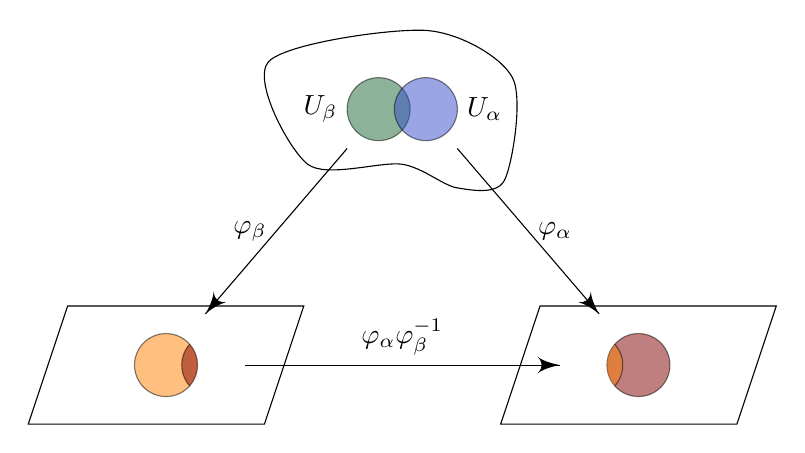
\begin{tikzpicture}
      \draw plot [smooth cycle] coordinates {(-1.2, -0.7) (0, -0.7) (0.7, -1) (1.3, -0.9) (1.4, 0.4) (0.3, 1) (-1.7, 0.6)};

      \draw (-0.3, 0) [fill=mgreen, opacity=0.5] circle [radius=0.4];
      \draw (0.3, 0) [fill=mblue, opacity=0.5] circle [radius=0.4];

      \node [left] at (-0.7, 0) {$U_\beta$};
      \node [right] at (0.7, 0) {$U_\alpha$};

      \begin{scope}[shift={(-4.75, -4)}]
        \draw (0, 0) -- (3, 0) -- (3.5, 1.5) -- (0.5, 1.5) -- cycle;

        \draw (1.75, 0.75) [fill=morange, opacity=0.5] circle [radius=0.4];
        \begin{scope}
          \clip (1.75, 0.75) circle [radius=0.4];
          \draw (2.35, 0.75) [fill=mred, opacity=0.5] circle [radius=0.4];
        \end{scope}
      \end{scope}

      \draw [->] (-0.7, -0.5) -- (-2.5, -2.6) node [pos=0.5, left] {$\varphi_\beta$};
      \draw [->] (0.7, -0.5) -- (2.5, -2.6) node [pos=0.5, right] {$\varphi_\alpha$};

      \begin{scope}[shift={(1.25, -4)}]
        \draw (0, 0) -- (3, 0) -- (3.5, 1.5) -- (0.5, 1.5) -- cycle;

        \draw (1.75, 0.75) [fill=mred, opacity=0.5] circle [radius=0.4];
        \begin{scope}
          \clip (1.75, 0.75) circle [radius=0.4];
          \draw (1.15, 0.75) [fill=morange, opacity=0.5] circle [radius=0.4];
        \end{scope}
      \end{scope}
      \draw [->] (-2, -3.25) -- (2, -3.25) node [pos=0.5, above] {$\varphi_\alpha \varphi_\beta^{-1}$};
    \end{tikzpicture}
  \end{center}
\end{defi}

\begin{defi}[Smooth map]\index{smooth map}
  Let $M$ be a manifold. Then a map $f: M \to \R$ is \emph{smooth} if it is smooth in each coordinate chart. Explicitly, for each chart $(U_\alpha, \varphi_\alpha)$, the composition $f \circ \varphi_\alpha^{-1}: \varphi_\alpha(U_\alpha) \to \R$ is smooth (in the usual sense)
  \begin{center}
    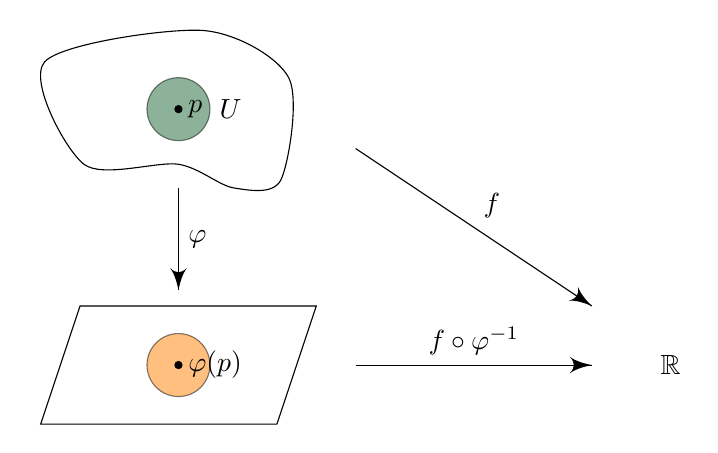
\begin{tikzpicture}
      \draw plot [smooth cycle] coordinates {(-1.2, -0.7) (0, -0.7) (0.7, -1) (1.3, -0.9) (1.4, 0.4) (0.3, 1) (-1.7, 0.6)};

      \draw [fill=mgreen, opacity=0.5] circle [radius=0.4];
      \node [right] {$p$};
      \node [circ] {};
      \node at (0.4, 0) [right] {$U$};

      \begin{scope}[shift={(-1.75, -4)}]
        \draw (0, 0) -- (3, 0) -- (3.5, 1.5) -- (0.5, 1.5) -- cycle;

        \draw (1.75, 0.75) [fill=morange, opacity=0.5] circle [radius=0.4];
        \node at (1.75, 0.75) [right] {$\varphi(p)$};
        \node at (1.75, 0.75) [circ] {};

        \draw [->] (4, 0.75) -- (7, 0.75) node [pos=0.5, above] {$f \circ \varphi^{-1}$};
        \node at (8, 0.75) {$\R$};
        \draw [->] (4, 3.5) -- (7, 1.5) node [pos=0.5, anchor = south west] {$f$};
      \end{scope}

      \draw [->] (0, -1) -- +(0, -1.3) node [pos=0.5, right] {$\varphi$};

    \end{tikzpicture}
  \end{center}
  More generally, if $M, N$ are manifolds, we say $f: M \to N$ is smooth if for any chart $(U, \varphi)$ of $M$ and any chart $(V, \xi)$ of $N$, the composition $\xi \circ f \circ \varphi^{-1}: \varphi(U) \to \xi(V)$ is smooth.
  \begin{center}
    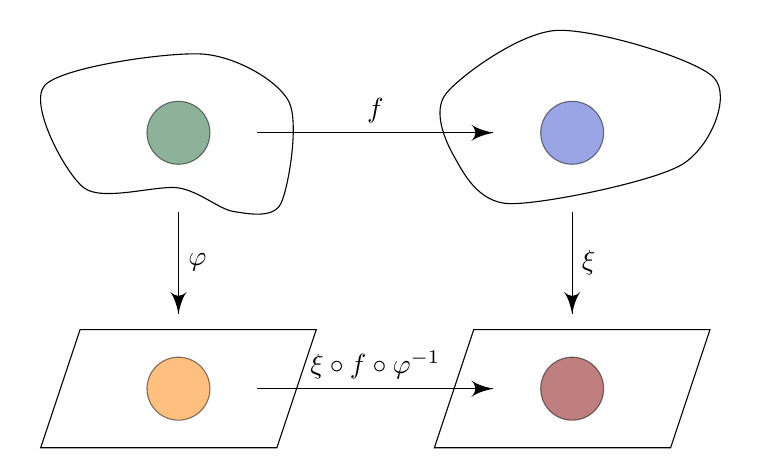
\begin{tikzpicture}
      \draw plot [smooth cycle] coordinates {(-1.2, -0.7) (0, -0.7) (0.7, -1) (1.3, -0.9) (1.4, 0.4) (0.3, 1) (-1.7, 0.6)};

      \draw [fill=mgreen, opacity=0.5] circle [radius=0.4];

      \begin{scope}[shift={(-1.75, -4)}]
        \draw (0, 0) -- (3, 0) -- (3.5, 1.5) -- (0.5, 1.5) -- cycle;

        \draw (1.75, 0.75) [fill=morange, opacity=0.5] circle [radius=0.4];
      \end{scope}

      \draw [->] (0, -1) -- +(0, -1.3) node [pos=0.5, right] {$\varphi$};
      \begin{scope}[shift={(5, 0)}]
        \draw plot [smooth cycle] coordinates {(1.4, -0.4) (-0.8, -0.9) (-1.5, -0.3) (-1.6, 0.5) (-0.2, 1.3) (1.8, 0.7)};

        \draw [fill=mblue, opacity=0.5] circle [radius=0.4];

        \begin{scope}[shift={(-1.75, -4)}]
          \draw (0, 0) -- (3, 0) -- (3.5, 1.5) -- (0.5, 1.5) -- cycle;

          \draw (1.75, 0.75) [fill=mred, opacity=0.5] circle [radius=0.4];
        \end{scope}

        \draw [->] (0, -1) -- +(0, -1.3) node [pos=0.5, right] {$\xi$};
      \end{scope}

      \draw [->] (1, 0) -- (4, 0) node [above, pos=0.5] {$f$};

      \draw [->] (1, -3.25) -- (4, -3.25) node [above, pos=0.5] {$\xi \circ f \circ \varphi^{-1}$};
    \end{tikzpicture}
  \end{center}
\end{defi}

Finally, we note that if $M, N$ are manifolds of dimensions $m$ and $n$ respectively, then $M \times N$ is a manifold of dimension $m + n$, where charts $(U, \varphi: U \to \R^m), (V, \xi: V \to \R^n)$ of $M$ and $N$ respectively give us a chart $\varphi \times \xi: U \times V \to \R^m \times \R^n = \R^{m + n}$ of $M \times N$.

All those definitions were made so that we can define what a Lie group is:

\begin{defi}[Lie group]\index{Lie group}
  A \emph{Lie group} is a group $G$ whose underlying set is given a manifold structure, and such that the multiplication map $m: G \times G \to G$ and inverse map $i: G \to G$ are smooth maps. We sometimes write $\mathcal{M}(G)$ for the underlying manifold of $G$.
\end{defi}

\begin{eg}
  The unit $2$-sphere
  \[
    S^2 = \{(x, y, z) \in \R^3: x^2 + y^2 + z^2 = 1\}
  \]
  is a manifold. Indeed, we can construct a coordinate patch near $N = (0, 0, 1)$. Near this point, we have $z = \sqrt{1 - x^2 - y^2}$. This works, since near the north pole, the $z$-coordinate is always positive. In this case, $x$ and $y$ are good coordinates near the north pole.

  However, it is a fact that the $2$-sphere $S^2$ has no Lie group structure.
\end{eg}

In general, most of our manifolds will be given by subsets of Euclidean space specified by certain equations, but note that not all subsets given by equations are manifolds! It is possible that they have some singularities.

\begin{defi}[Dimension of Lie group]\index{Dimension of Lie group}\index{Lie group!dimension}
  The \emph{dimension} of a Lie group $G$ is the dimension of the underlying manifold.
\end{defi}

\begin{defi}[Subgroup]\index{subgroup}
  A \emph{subgroup} $H$ of $G$ is a subset of $G$ that is also a group under the same operations. We write $H \leq G$ if $H$ is a subgroup of $G$.
\end{defi}

The really interesting thing is when the subgroup is also a manifold!
\begin{defi}[Lie subgroup]\index{Lie subgroup}
  A subgroup is a \emph{Lie subgroup} if it is also a manifold (under the induced smooth structure).
\end{defi}

%Given a Lie group $G$, we can introduce coordinates $\boldsymbol\theta = \{\theta^i\}_{i = 1, \ldots, D}$, where $D = \dim(G)$, in a patch $P$ containing $e$. We write $g(\boldsymbol\theta) \in G$ for the element of $G$ specified by the coordinates $\boldsymbol\theta$. We by convention set $g(0) = e$.
%
%Suppose we have two elements $g(\boldsymbol\theta), g(\boldsymbol\theta') \in G$. Suppose they are small enough so that their product is also in the patch $P$. So we an write
%\[
% g(\boldsymbol\theta) g(\boldsymbol\theta') = g(\boldsymbol\varphi)
%\]
%This corresponds to a smooth map $G \times G \to G$. In coordinates, we can write this as
%\[
% \varphi^i = \varphi^i(\boldsymbol\theta, \boldsymbol\theta').
%\]
%This map is smooth.
%
%Similarly, group inversion also defines a smooth map.

We now look at some examples.
\begin{eg}
  Let $G = (\R^D, +)$ be the $D$-dimensional Euclidean space with addition as the group operation. The inverse of a vector $\mathbf{x}$ is $-\mathbf{x}$, and the identity is $\mathbf{0}$. This is obviously locally homeomorphic to $\R^D$, since it \emph{is} $\R^D$, and addition and negation are obviously smooth.
\end{eg}

This is a rather boring example, since $\R^D$ is a rather trivial manifold, and the operation is commutative. The largest source of examples we have will be matrix Lie groups.

\subsection{Matrix Lie groups}
We write $\Mat_n(\F)$ for the set of $n\times n$ matrices with entries in a field $\F$ (usually $\R$ or $\C$). Matrix multiplication is certainly associative, and has an identity, namely the identity $I$. However, it doesn't always have inverses --- not all matrices are invertible! So this is not a group (instead, we call it a monoid). Thus, we are led to consider the \emph{general linear group}:

\begin{defi}[General linear group]\index{general linear group}
  The \emph{general linear group} is
  \[
    \GL(n, \F) = \{M \in \Mat_n(\F): \det M \not= 0\}.
  \]
\end{defi}
This is closed under multiplication since the determinant is multiplicative, and matrices with non-zero determinant are invertible.

\begin{defi}[Special linear group]\index{special linear group}
  The \emph{special linear group} is
  \[
    \SL(n, \F) = \{M \in \Mat_n(\F): \det M =1\} \leq \GL(n, \F).
  \]
\end{defi}
While these are obviously groups, less obviously, these are in fact Lie groups! In the remainder of the section, we are going to casually claim that all our favorite matrix groups are Lie groups. Proving these take some work and machinery, and we will not bother ourselves with that too much. However, we can do it explicitly for certain special cases:

\begin{eg}
  Explicitly, we can write
  \[
    \SL(2, \R) = \left\{
      \begin{pmatrix}
        a & b\\
        c & d
      \end{pmatrix}:
    a, b, c, d \in \R, ad - bc = 1\right\}.
  \]
  The identity is the matrix with $a = d = 1$ and $b = c = 0$. For $a \not= 0$, we have
  \[
    d = \frac{1 + bc}{a}.
  \]
  This gives us a coordinate patch for all points where $a \not= 0$ in terms of $b, c, a$, which, in particular, contains the identity $I$. By considering the case where $b \not= 0$, we obtain a separate coordinate chart, and these together cover all of $\SL(2, \R)$, as a matrix in $\SL(2, \R)$ cannot have $a = b = 0$.

  Thus, we see that $\SL(2, \R)$ has dimension $3$.
\end{eg}

In general, by a similar counting argument, we have
\begin{align*}
  \dim (\SL(n, \R)) &= n^2 - 1& \dim (\SL(n, \C)) &= 2n^2 - 2\\
  \dim (\GL(n, \R)) &= n^2,& \dim(\GL(n, \C)) &= 2n^2.
\end{align*}
Most of the time, we are interested in matrix Lie groups, which will be subgroups of $\GL(n, \R)$.

\subsubsection*{Subgroups of \texorpdfstring{$\GL(n, \R)$}{GL(n, R)}}
\begin{lemma}
  The \term{general linear group}\index{$\GL(n, \R)$}:
  \[
    \GL(n, \R) = \{M \in \Mat_n(\R): \det M \not= 0\}
  \]
  and \term{orthogonal group}\index{$\Or(n)$}:
  \[
    \Or(n) = \{M \in \GL(n, \R): M^TM = I\}
  \]
  are Lie groups.
\end{lemma}
Note that we write $\Or(n)$ instead of $\Or(n, \R)$ since orthogonal matrices make sense only when talking about real matrices.

The orthogonal matrices are those that preserve the lengths of vectors. Indeed, for $\mathbf{v}\in \R^n$, we have
\[
  |M\mathbf{v}|^2 = \mathbf{v}^T M^T M \mathbf{v} = \mathbf{v}^T \mathbf{v} = |\mathbf{v}|^2.
\]
We notice something interesting. If $M \in \Or(n)$, we have
\[
  1 = \det(I) = \det(M^TM) = \det(M)^2.
\]
So $\det(M) = \pm 1$. Now $\det$ is a continuous function, and it is easy to see that $\det$ takes both $\pm 1$. So $\Or(n)$ has (at least) two connected components. Only one of these pieces contains the identity, namely the piece $\det M = 1$. We might expect this to be a group on its own right, and indeed it is, because $\det$ is multiplicative.
\begin{lemma}
  The \term{special orthogonal group} \term{$\SO(n)$}:
  \[
    \SO(n) = \{M \in \Or(n): \det M = 1\}
  \]
  is a Lie group.
\end{lemma}

Given a frame $\{\mathbf{v}_1, \cdots, \mathbf{v}_n\}$ in $\R^n$ (i.e.\ an ordered basis), any orthogonal matrix $M \in \Or(n)$ acts on it to give another frame $\mathbf{v}_a \in \R^n \mapsto \mathbf{v}_a' \mapsto M\mathbf{v}_a \in \R^n$.
\begin{defi}[Volume element]\index{volume element}
  Given a frame $\{\mathbf{v}_1, \cdots, \mathbf{v}_n\}$ in $\R^n$, the \emph{volume element} is
  \[
    \Omega = \varepsilon_{i_1 \ldots i_n} v_1^{i_1} v_2^{i_2} \cdots v_n^{i_n}.
  \]
\end{defi}

By direct computation, we see that an orthogonal matrix preserves the sign of the volume element iff its determinant is $+1$, i.e.\ $M \in \SO(n)$.

We now want to find a more explicit description of these Lie groups, at least in low dimensions. Often, it is helpful to classify these matrices by their eigenvalues:

\begin{defi}[Eigenvalue]\index{eigenvalue}
  A complex number $\lambda$ is an \emph{eigenvalue} of $M \in M(n)$ if there is some (possibly complex) vector $\mathbf{v}_\lambda \not= 0$ such that
  \[
    M \mathbf{v}_\lambda = \lambda \mathbf{v}_\lambda.
  \]
\end{defi}

\begin{thm}
  Let $M$ be a real matrix. Then $\lambda$ is an eigenvalue iff $\lambda^*$ is an eigenvalue. Moreover, if $M$ is orthogonal, then $|\lambda|^2 = 1$.
\end{thm}

\begin{proof}
  Suppose $M \mathbf{v}_\lambda = \lambda \mathbf{v}_\lambda$. Then applying the complex conjugate gives $M \mathbf{v}_\lambda^* = \lambda^* \mathbf{v}_\lambda^*$.

  Now suppose $M$ is orthogonal. Then $M\mathbf{v}_\lambda = \lambda \mathbf{v}_\lambda$ for some non-zero $\mathbf{v}_\lambda$. We take the norm to obtain $|M\mathbf{v}_\lambda| = |\lambda| |\mathbf{v}_\lambda|$. Using the fact that $|\mathbf{v}_\lambda| = |M\mathbf{v}_\lambda|$, we have $|\lambda| = 1$. So done.
\end{proof}

\begin{eg}
  Let $M \in \SO(2)$. Since $\det M = 1$, the eigenvalues must be of the form $\lambda = e^{i\theta}, e^{-i\theta}$. In this case, we have
  \[
    M = M(\theta) =
    \begin{pmatrix}
      \cos \theta & -\sin \theta\\
      \sin \theta & \cos \theta
    \end{pmatrix},
  \]
  where $\theta$ is the rotation angle in $S^1$. Here we have
  \[
    M(\theta_1)M(\theta_2) = M(\theta_2) M(\theta_1) = M(\theta_1 + \theta_2).
  \]
  So we have $\mathcal{M}(\SO(2)) = S^1$.
\end{eg}

\begin{eg}
  Consider $G = \SO(3)$. Suppose $M \in \SO(3)$. Since $\det M = +1$, and the eigenvalues have to come in complex conjugate pairs, we know one of them must be $1$. Then the other two must be of the form $e^{i\theta}, e^{-i\theta}$, where $\theta \in S^1$.

  We pick a normalized eigenvector $\mathbf{n}$ for $\lambda = 1$. Then $M\mathbf{n} = \mathbf{n}$, and $\mathbf{n} \cdot \mathbf{n} = 1$. This is known as the \emph{axis of rotation}. Similarly, $\theta$ is the angle of rotation. We write $M(\mathbf{n}, \theta)$ for this matrix, and it turns out this is
  \[
    M(\mathbf{n}, \theta)_{ij} = \cos \theta \delta_{ij} + (1 - \cos \theta)n_i n_j - \sin \theta \varepsilon_{ijk} n_k.
  \]
  Note that this does not uniquely specify a matrix. We have
  \[
    M(\mathbf{n}, 2\pi - \theta) = M(-\mathbf{n}, \theta).
  \]
  Thus, to uniquely specify a matrix, we need to restrict the range of $\theta$ to $0 \leq \theta \leq \pi$, with the further identification that
  \[
    (\mathbf{n}, \pi) \sim (-\mathbf{n}, \pi).
  \]
  Also note that $M(\mathbf{n}, 0) = I$ for any $\mathbf{n}$.

  Given such a matrix, we can produce a vector $\mathbf{w} = \theta \mathbf{n}$. Then $\mathbf{w}$ lies in the region
  \[
    B_3 = \{\mathbf{w} \in \R^3: \norm{\mathbf{w}} \leq \pi\} \subseteq \R^3.
  \]
  This has a boundary
  \[
    \partial B_3 = \{\mathbf{w} \in \R^3: \norm{\mathbf{w}} = \pi\} \cong S^2.
  \]
  Now we identify antipodal points on $\partial B_3$. Then each vector in the resulting space corresponds to exactly one element of $\SO(3)$.
\end{eg}

\subsubsection*{Subgroups of \texorpdfstring{$\GL(n, \C)$}{GL(n, C)}}
We can similarly consider subgroups of $\GL(n, \C)$. Common examples include
\begin{defi}[Unitary group]\index{unitary group}\index{$\U(n)$}
  The \emph{unitary group} is defined by
  \[
    \U(n) = \{U \in \GL(n, \C): U^\dagger U = I\}.
  \]
\end{defi}
These are important in physics, because unitary matrices are exactly those that preserve the norms of vectors, namely $\norm{\mathbf{v}} = \norm{U\mathbf{v}}$ for all $\mathbf{v}$.

Again, if $U^\dagger U = 1$, then $|\det(U)|^2 = 1$. So $\det U = e^{i\delta}$ for some $\delta \in \R$. Unlike the real case, the determinant can now take a continuous range of values, and this no longer disconnects the group. In fact, $\U(n)$ is indeed connected.

\begin{defi}[Special unitary group]\index{special unitary group}\index{$\SU(n)$}
  The \emph{special unitary group} is defined by
  \[
    \SU(n) = \{U \in \U(n): \det U = 1\}.
  \]
\end{defi}

It is an easy exercise to show that
\[
  \dim[\U(n)] = 2n^2 - n^2 = n^2.
\]
For $\SU(n)$, the determinant condition imposes an additional single constraint, so we have
\[
  \dim[\SU(n)] = n^2 - 1.
\]
\begin{eg}
  Consider the group $G = \U(1)$. This is given by
  \[
    \U(1) = \{z \in \C: |z| = 1\}.
  \]
  Therefore we have
  \[
    \mathcal{M}[\U(1)] = S^1.
  \]
  However, we also know another Lie group with underlying manifold $S^1$, namely $\SO(2)$. So are they ``the same''?
\end{eg}

\subsection{Properties of Lie groups}
The first thing we want to consider is when two Lie groups are ``the same''. We take the obvious definition of isomorphism.
\begin{defi}[Homomorphism of Lie groups]\index{homomorphism of Lie groups}\index{Lie group!homomorphism}
  Let $G, H$ be Lie groups. A map $J: G \to H$ is a \emph{homomorphism} if it is smooth and for all $g_1, g_2 \in G$, we have
  \[
    J(g_1 g_2) = J(g_1) J(g_2).
  \]
  (the second condition says it is a homomorphism of groups)
\end{defi}

\begin{defi}[Isomorphic Lie groups]\index{isomorphism of Lie groups}\index{Lie groups!isomorphism}
  An \emph{isomorphism} of Lie groups is a bijective homomorphism whose inverse is also a homomorphism. Two Lie groups are \emph{isomorphic} if there is an isomorphism between them.
\end{defi}

\begin{eg}
  We define the map $J: \U(1) \to \SO(2)$ by
  \[
    J(e^{i\theta}) \mapsto
    \begin{pmatrix}
      \cos \theta & -\sin \theta\\
      \sin \theta & \cos \theta
    \end{pmatrix} \in \SO(2).
  \]
  This is easily seen to be a homomorphism, and we can construct an inverse similarly.
\end{eg}

\begin{ex}
  Show that $\mathcal{M}(\SO(2)) \cong S^3$.
\end{ex}

We now look at some words that describe manifolds. Usually, manifolds that satisfy these properties are considered nice.

The first notion is the idea of compactness. The actual definition is a bit weird and takes time to get used to, but there is an equivalent characterization if the manifold is a subset of $\R^n$.
\begin{defi}[Compact]\index{compact}
  A manifold (or topological space) $X$ is \emph{compact} if every open cover of $X$ has a finite subcover.

  If the manifold is a subspace of some $\R^n$, then it is compact iff it is closed and bounded.
\end{defi}

\begin{eg}
  The sphere $S^2$ is compact, but the hyperboloid given by $x^2 - y^2 - z^2 = 1$ (as a subset of $\R^3$) is not.
\end{eg}

\begin{eg}
  The orthogonal groups are compact. Recall that the definition of an orthogonal matrix requires $M^T M = I$. Since this is given by a polynomial equation in the entries, it is closed. It is also bounded since each entry of $M$ has magnitude at most $1$.

  Similarly, the special orthogonal groups are compact.
\end{eg}

\begin{eg}
  Sometimes we want to study more exciting spaces such as Minkowski spaces. Let $n = p + q$, and consider the matrices that preserve the metric on $\R^n$ of signature $(p, q)$, namely
  \[
    \Or(p, q) = \{M \in \GL(n, \R): M^T \eta M = \eta\},
  \]
  where
  \[
    \eta =
    \begin{pmatrix}
      I_p & 0\\
      0 & -I_q
    \end{pmatrix}.
  \]
  For $p, q$ both non-zero, this group is non-compact. For example, if we take $\SO(1, 1)$, then the matrices are all of the form
  \[
    M =
    \begin{pmatrix}
      \cosh\theta & \sinh \theta\\
      \sinh \theta & \cosh \theta
    \end{pmatrix},
  \]
  where $\theta \in \R$. So this space is homeomorphic to $\R$, which is not compact.

  Another common example of a non-compact group is the \term{Lorentz group} $\Or(3, 1)$.
\end{eg}

Another important property is simply-connectedness.
\begin{defi}[Simply connected]\index{simply connected}
  A manifold $M$ is \emph{simply connected} if it is connected (there is a path between any two points), and every loop $l: S^1 \to M$ can be contracted to a point. Equivalently, any two paths between any two points can be continuously deformed into each other.
\end{defi}

\begin{eg}
  The circle $S^1$ is not simply connected, as the loop that goes around the circle once cannot be continuously deformed to the loop that does nothing (this is non-trivial to prove).
\end{eg}

\begin{eg}
  The $2$-sphere $S^2$ is simply connected, but the torus is not. $\SO(3)$ is also not simply connected. We can define the map by
  \[
    l(\theta) =
    \begin{cases}
      \theta \mathbf{n} & \theta \in [0, \pi)\\
      -(2\pi - \theta) \mathbf{n} & \theta \in [\pi, 2\pi)
    \end{cases}
  \]
  This is indeed a valid path because we identify antipodal points.
\end{eg}

The failure of simply-connectedness is measured by the \emph{fundamental group}.
\begin{defi}[Fundamental group/First homotopy group]\index{fundamental group}\index{homotopy group}\index{first homotopy group}
  Let $M$ be a manifold, and $x_0 \in M$ be a preferred point. We define $\pi_1(M)$ to be the equivalence classes of loops starting and ending at $x_0$, where two loops are considered equivalent if they can be continuously deformed into each other.

  This has a group structure, with the identity given by the ``loop'' that stays at $x_0$ all the time, and composition given by doing one after the other.
\end{defi}

\begin{eg}
  $\pi_1(S^2) = \{0\}$ and $\pi_1(T^2) = \Z \times \Z$. We also have $\pi_1(\SO(2)) = \Z/2\Z$. We will not prove these results.
\end{eg}


\section{Lie algebras}
It turns out that in general, the study of a Lie group can be greatly simplified by studying its associated \emph{Lie algebra}, which can be thought of as an infinitesimal neighbourhood of the identity in the Lie group.

To get to that stage, we need to develop some theory of Lie algebra, and also of differentiation.

\subsection{Lie algebras}
We begin with a rather formal and weird definition of a Lie algebra.

\begin{defi}[Lie algebra]\index{Lie algebra}
  A \emph{Lie algebra} $\mathfrak{g}$ is a vector space (over $\R$ or $\C$) with a \term{bracket}
  \[
    [\ph,\ph] : \mathfrak{g} \times \mathfrak{g} \to \mathfrak{g}
  \]
  satisfying
  \begin{enumerate}
    \item $[X, Y] = -[Y, X]$ for all $X, Y \in \mathfrak{g}$ \hfill(antisymmetry)
    \item $[\alpha X + \beta Y, Z] = \alpha [X, Z] + \beta [Y, Z]$ for all $X, Y, Z \in \mathfrak{g}$ and $\alpha, \beta \in \F$ \hfill((bi)linearity)
    \item $[X, [Y, Z]] + [Y, [Z, X]] + [Z, [X, Y]] = 0$ for all $X, Y, Z \in \mathfrak{g}$.\hfill(Jacobi identity\index{Jacobi identity})
  \end{enumerate}
  Note that linearity in the second argument follows from linearity in the first argument and antisymmetry.
\end{defi}
Some (annoying) pure mathematicians will complain that we should state anti-symmetry as $[X, X] = 0$ instead, which is a stronger condition if we are working over a field of characteristic $2$, but I do not care about such fields.

There isn't much one can say to motivate the Jacobi identity. It is a property that our naturally-occurring Lie algebras have, and turns out to be useful when we want to prove things about Lie algebras.

\begin{eg}
  Suppose we have a vector space $V$ with an associative product (e.g.\ a space of matrices with matrix multiplication). We can then turn $V$ into a Lie algebra by defining
  \[
    [X, Y] = XY - YX.
  \]
  We can then prove the axioms by writing out the expressions.
\end{eg}

\begin{defi}[Dimension of Lie algebra]\index{dimension of Lie algebra}\index{Lie algebra!dimension}
  The \emph{dimension} of a Lie algebra is the dimension of the underlying vector space.
\end{defi}

Given a finite-dimensional Lie algebra, we can pick a basis $\mathcal{B}$ for $\mathfrak{g}$.
\[
  \mathcal{B} = \{T^a: a = 1, \cdots, \dim \mathfrak{g}\}.
\]
Then any $X \in \mathfrak{g}$ can be written as
\[
  X = X_a T^a = \sum_{a = 1}^n X_a T^a,
\]
where $X_a \in \F$ and $n = \dim \mathfrak{g}$.

By linearity, the bracket of elements $X, Y \in \mathfrak{g}$ can be computed via
\[
  [X, Y] = X_a Y_b [T^a, T^b].
\]
In other words, the whole structure of the Lie algebra can be given by the bracket of basis vectors. We know that $[T^a, T^b]$ is again an element of $\mathfrak{g}$. So we can write
\[
  [T^a, T^b] = f^{ab}\!_c T^c,
\]
where $f^{ab}\!_c\in \F$ are the \emph{structure constants}.
\begin{defi}[Structure constants]\index{structure constants}
  Given a Lie algebra $\mathfrak{g}$ with a basis $\mathcal{B} = \{T^a\}$, the \emph{structure constants} are $f^{ab}\!_c$ given by
  \[
    [T^a, T^b] = f^{ab}\!_c T^c,
  \]
\end{defi}

By the antisymmetry of the bracket, we know
\begin{prop}
  \[
    f^{ba}\!_c = -f^{ab}\!_c.
  \]
\end{prop}

By writing out the Jacobi identity, we obtain
\begin{prop}
  \[
    f^{ab}\!_c f^{cd}\!_e + f^{da}\!_c f^{cb}\!_e + f^{bd}\!_c f^{ca}\!_e = 0.
  \]
\end{prop}

As before, we would like to know when two Lie algebras are the same.
\begin{defi}[Homomorphism of Lie algebras]\index{homomorphism of Lie algebras}
  A \emph{homomorphism} of Lie algebras $\mathfrak{g}, \mathfrak{h}$ is a linear map $f: \mathfrak{g} \to \mathfrak{h}$ such that
  \[
    [f(X), f(Y)] = f([X, Y]).
  \]
\end{defi}

\begin{defi}[Isomorphism of Lie algebras]\index{isomorphism of Lie algebras}\index{Lie algebra!isomorphism}
  An \emph{isomorphism} of Lie algebras is a homomorphism with an inverse that is also a homomorphism. Two Lie algebras are \emph{isomorphic} if there is an isomorphism between them.
\end{defi}

Similar to how we can have a subgroup, we can also have a subalgebra $\mathfrak{h}$ of $\mathfrak{g}$.

\begin{defi}[Subalgebra]\index{subalgebra}\index{Lie algebra!subalgebra}
  A \emph{subalgebra} of a Lie algebra $\mathfrak{g}$ is a vector subspace that is also a Lie algebra under the bracket.
\end{defi}

Recall that in group theory, we have a stronger notion of a normal subgroup, which are subgroups invariant under conjugation. There is an analogous notion for subalgebras.
\begin{defi}[Ideal]\index{ideal of Lie algebra}\index{Lie algebra!ideal}\index{Lie algebra!invariant subalgebra}\index{invariant subalgebra}
  An \emph{ideal} of a Lie algebra $\mathfrak{g}$ is a subalgebra $\mathfrak{h}$ such that $[X, Y] \in \mathfrak{h}$ for all $X \in \mathfrak{g}$ and $Y \in \mathfrak{h}$.
\end{defi}

\begin{eg}
  Every Lie algebra $\mathfrak{g}$ has two \emph{trivial}\index{trivial ideal}\index{ideal!trivial} ideals $\mathfrak{h} = \{0\}$ and $\mathfrak{h} = \mathfrak{g}$.
\end{eg}

\begin{defi}[Derived algebra]
  The \term{derived algebra} of a Lie algebra $\mathfrak{g}$ is
  \[
    \mathfrak{i} = [\mathfrak{g}, \mathfrak{g}] = \spn_\F\{[X, Y]: X, Y \in \mathfrak{g}\},
  \]
  where $\F = \R$ or $\C$ depending on the underlying field.
\end{defi}
It is clear that this is an ideal. Note that this may or may not be trivial.

\begin{defi}[Center of Lie algebra]\index{center of Lie algebra}\index{Lie algebra!center}
  The \emph{center} of a Lie algebra $\mathfrak{g}$ is given by
  \[
    \xi(\mathfrak{g}) = \{X \in \mathfrak{g}: [X, Y] = 0\text{ for all }Y \in \mathfrak{g}\}.
  \]
\end{defi}
This is an ideal, by the Jacobi identity.

\begin{defi}[Abelian Lie algebra]\index{abelian Lie algebra}\index{Lie algebra!abelian}
  A Lie algebra $\mathfrak{g}$ is \emph{abelian} if $[X, Y] = 0$ for all $X, Y \in \mathfrak{g}$. Equivalently, if $\xi(\mathfrak{g}) = \mathfrak{g}$.
\end{defi}

\begin{defi}[Simple Lie algebra]\index{simple Lie algebra}\index{Lie algebra!simple}
  A \emph{simple Lie algebra} is a Lie algebra $\mathfrak{g}$ that is non-abelian and possesses no non-trivial ideals.
\end{defi}
If $\mathfrak{g}$ is simple, then since the center is always an ideal, and it is not $\mathfrak{g}$ since $\mathfrak{g}$ is not abelian, we must have $\xi(\mathfrak{g}) = \{0\}$. On the other hand, the derived algebra is also an ideal, and is non-zero since it is not abelian. So we must have $\mathfrak{i}(\mathfrak{g}) = \mathfrak{g}$.

We will later see that these are the Lie algebras on which we can define a non-degenerate invariant inner product. In fact, there is a more general class, known as the \emph{semi-simple} Lie algebras, that are exactly those for which non-degenerate invariant inner products can exist.

These are important in physics because, as we will later see, to define the Lagrangian of a gauge theory, we need to have a non-degenerate invariant inner product on the Lie algebra. In other words, we need a (semi-)simple Lie algebra.


\subsection{Differentiation}
We are eventually going to get a Lie algebra from a Lie group. This is obtained by looking at the tangent vectors at the identity. When we have homomorphisms $f: G \to H$ of Lie groups, they are in particular smooth, and taking the derivative will give us a map from tangent vectors in $G$ to tangent vectors in $H$, which in turn restricts to a map of their Lie algebras. So we need to understand how differentiation works.

Before that, we need to understand how tangent vectors work. This is completely general and can be done for manifolds which are not necessarily Lie groups. Let $M$ be a smooth manifold of dimension $D$ and $p \in M$ a point. We want to formulate a notion of a ``tangent vector'' at the point $p$. We know how we can do this if the space is $\R^n$ --- a tangent vector is just any vector in $\R^n$. By definition of a manifold, near a point $p$, the manifold looks just like $\R^n$. So we can just pretend it is $\R^n$, and use tangent vectors in $\R^n$.

However, this definition of a tangent vector requires us to pick a particular coordinate chart. It would be nice to have a more ``intrinsic'' notion of vectors. Recall that in $\R^n$, if we have a function $f: \R^n \to \R$ and a tangent vector $\mathbf{v}$ at $p$, then we can ask for the directional derivative of $f$ along $\mathbf{v}$. We have a correspondence
\[
  \mathbf{v} \longleftrightarrow \frac{\partial}{\partial \mathbf{v}}.
\]
This directional derivative takes in a function and returns its derivative at a point, and is sort-of an ``intrinsic'' notion. Thus, instead of talking about $\mathbf{v}$, we will talk about the associated directional derivative $\frac{\partial}{\partial \mathbf{v}}$.

It turns out the characterizing property of this directional derivative is the product rule:
\[
  \frac{\partial}{\partial \mathbf{v}}(fg) = f(p) \frac{\partial}{\partial \mathbf{v}} g + g(p) \frac{\partial}{\partial \mathbf{v}}f.
\]
So a ``directional derivative'' is a linear map from the space of smooth functions $M \to \R$ to $\R$ that satisfies the Leibnitz rule.
\begin{defi}[Tangent vector]\index{tangent vector}
  Let $M$ be a manifold and write $C^\infty(M)$ for the vector space of smooth functions on $M$. For $p \in M$, a \emph{tangent vector} is a linear map $v: C^\infty(M) \to \R$ such that for any $f, g \in C^\infty(M)$, we have
  \[
    v(fg) = f(p) v(g) + v(f) g(p).
  \]
  It is clear that this forms a vector space, and we write $T_p M$ for the vector space of tangent vectors at $p$.
\end{defi}
Now of course one would be worried that this definition is too inclusive, in that we might have included things that are not genuinely directional derivatives. Fortunately, this is not the case, as the following proposition tells us.

In the case where $M$ is a submanifold of $\R^n$, we can identify the tangent space with an actual linear subspace of $\R^n$. This is easily visualized when $M$ is a surface in $\R^3$, where the tangent vectors consists of the vectors in $\R^3$ ``parallel to'' the surface at the point, and in general, a ``direction'' in $M$ is also a ``direction'' in $\R^n$, and tangent vectors of $\R^n$ can be easily identified with elements of $\R^n$ in the usual way.

This will be useful when we study matrix Lie groups, because this means the tangent space will consist of matrices again.
\begin{prop}
  Let $M$ be a manifold with local coordinates $\{x^i\}_{i = 1, \cdots, D}$ for some region $U \subseteq M$ containing $p$. Then $T_p M$ has basis
  \[
    \left\{\frac{\partial}{\partial x^j}\right\}_{j = 1, \cdots, D}.
  \]
  In particular, $\dim T_p M = \dim M$.
\end{prop}
This result on the dimension is extremely useful. Usually, we can manage to find a bunch of things that we know lie in the tangent space, and to show that we have found all of them, we simply count the dimensions.

One way we can obtain tangent vectors is by differentiating a curve.
\begin{defi}[Smooth curve]\index{smooth curve}
  A \emph{smooth curve} is a smooth map $\gamma: \R \to M$. More generally, a \emph{curve} is a $C^1$ function $\R \to M$.
\end{defi}
Since we only want the first derivative, being $C^1$ is good enough.

There are two ways we can try to define the derivative of the curve at time $t = 0 \in \R$. Using the definition of a tangent vector, to specify $\dot{\gamma}(0)$ is to tell how we can differentiate a function $f: M \to \R$ at $p = \gamma(0)$ in the direction of $\dot{\gamma}(0)$. This is easy. We define
\[
  \dot{\gamma}(0)(f) = \frac{\d}{\d t} f(\gamma(t)) \in \R.
\]
If this seems too abstract, we can also do it in local coordinates.

We introduce some coordinates $\{x_i\}$ near $p \in M$. We then refer to $\gamma$ by coordinates (at least near $p$), by
\[
  \gamma: t \in \R \mapsto \{x^i(t) \in \R: i = 1, \cdots, D\}.
\]
By the smoothness condition, we know $x^i(t)$ is differentiable, with $x^i(0) = 0$. Then the \emph{tangent vector} of the curve $\gamma$ at $p$ is
\[
  v_\gamma = \dot{x}^i(0) \frac{\partial}{\partial x^i} \in T_p (M),\quad \dot{x}^i(t) = \frac{\d x^i}{\d t}.
\]
It follows from the chain rule that this exactly the same thing as what we described before.

More generally, we can define the derivative of a map between manifolds.
\begin{defi}[Derivative]\index{derivative}
  Let $f: M \to N$ be a map between manifolds. The \emph{derivative} of $f$ at $p \in M$ is the linear map
  \[
    \D f_p: T_p M \to T_{f(p)} N
  \]
  given by the formula
  \[
    (\D f_p)(v)(g) = v(g \circ f)
  \]
  for $v \in T_p M$ and $g \in C^\infty(N)$.
\end{defi}
This will be useful later when we want to get a map of Lie algebras from a map of Lie groups.

\subsection{Lie algebras from Lie groups}
We now try to get a Lie algebra from a Lie group $G$, by considering $T_e(G)$.

\begin{thm}
  The tangent space of a Lie group $G$ at the identity naturally admits a Lie bracket
  \[
    [\ph, \ph]: T_e G \times T_e G \to T_e G
  \]
  such that
  \[
    \mathcal{L}(G) = (T_e G, [\ph, \ph])
  \]
  is a Lie algebra.
\end{thm}

\begin{defi}[Lie algebra of a Lie group]\index{Lie algebra of a Lie group}
  Let $G$ be a Lie group. The \emph{Lie algebra} of $G$, written $\mathcal{L}(G)$ or $\mathfrak{g}$, is the tangent space $T_e G$ under the natural Lie bracket.
\end{defi}
The general convention is that if the name of a Lie group is in upper case letters, then the corresponding Lie algebra is the same name with lower case letters in fraktur font. For example, the Lie group of $\SO(n)$ is $\so(n)$.

\begin{proof}
  We will only prove it for the case of a matrix Lie group $G \subseteq \Mat_n(\F)$. Then $T_I G$ can be naturally identified as a subspace of $\Mat_n(\F)$. There is then an obvious candidate for the Lie bracket --- the actual commutator:
  \[
    [X, Y] = XY - YX.
  \]
  The basic axioms of a Lie algebra can be easily (but painfully) checked.

  However, we are not yet done. We have to check that if we take the bracket of two elements in $T_I(G)$, then it still stays within $T_I(G)$. This will be done by producing a curve in $G$ whose derivative at $0$ is the commutator $[X, Y]$.

  In general, let $\gamma$ be a smooth curve in $G$ with $\gamma(0) = I$. Then we can Taylor expand
  \[
    \gamma(t) = I + \dot{\gamma}(0) t + \ddot{\gamma}(0) t^2 + O(t^3),
  \]
  Now given $X, Y \in T_e G$, we take curves $\gamma_1, \gamma_2$ such that $\dot{\gamma}_1(0) = X$ and $\dot{\gamma}_2(0) = Y$. Consider the curve given by
  \[
    \gamma(t) = \gamma_1^{-1}(t) \gamma_2^{-1}(t) \gamma_1(t)\gamma_2(t) \in G.
  \]
  We can Taylor expand this to find that
  \[
    \gamma(t) = I + [X, Y] t^2 + O(t^3).
  \]
  This isn't too helpful, as $[X, Y]$ is not the coefficient of $t$. We now do the slightly dodgy step, where we consider the curve
  \[
    \tilde{\gamma}(t) = \gamma(\sqrt{t}) = I + [X, Y] t + O(t^{3/2}).
  \]
  Now this is only defined for $t \geq 0$, but it is good enough, and we see that its derivative at $t = 0$ is $[X, Y]$. So the commutator is in $T_I(G)$. So we know that $\mathcal{L}(G)$ is a Lie algebra.
\end{proof}

\begin{eg}
  Let $G = \GL(n, \F)$, where $\F = \R$ or $\C$. Then $\mathcal{L}(\GL(n, \F)) = \gl(n, \F) = \Mat_n(\F)$ because we know it must be an $n \times n$-dimensional subspace of $\Mat_n(\F)$.

  More generally, for a vector space $V$, say of dimension $n$, we can consider the group of invertible linear maps $V \to V$, written $\GL(V)$. By picking a basis of $V$, we can construct an isomorphism $\GL(V) \cong \GL(n, \F)$, and this gives us a smooth structure on $\GL(V)$ (this does not depend on the basis chosen). Then the Lie algebra $\gl(V)$ is the collection of all linear maps $V \to V$.
\end{eg}

\begin{eg}
  If $G = \SO(2)$, then the curves are of the form
  \[
    g(t) = M(\theta(t)) =
    \begin{pmatrix}
      \cos \theta(t) & -\sin \theta (t)\\
      \sin \theta(t) & \cos \theta(t)
    \end{pmatrix} \in \SO(2).
  \]
  So we have
  \[
    \dot{g}(0) =
    \begin{pmatrix}
      0 & -1\\
      1 & 0
    \end{pmatrix} \dot{\theta}(0).
  \]
  Since the Lie algebra has dimension $1$, these are all the matrices in the Lie algebra. So the Lie algebra is given by
  \[
    \so(2) = \left\{
      \begin{pmatrix}
        0 & -c\\
        c & 0
      \end{pmatrix}, c \in \R
    \right\}.
  \]
\end{eg}

\begin{eg}
  More generally, suppose $G = \SO(n)$, and we have a path $R(t) \in \SO(n)$.

  By definition, we have
  \[
    R^T(t) R(t) = I.
  \]
  Differentiating gives
  \[
    \dot{R}^T(t) R(t) + R^T(t) \dot{R}(t) = 0.
  \]
  for all $t \in \R$. Evaluating at $t = 0$, and noting that $R(0) = I$, we have
  \[
    X^T + X = 0,
  \]
  where $X = \dot{R}(0)$ is a tangent vector. There are no further constraints from demanding that $\det R = +1$, since this is obeyed anyway for any matrix in $\Or(n)$ near $I$.

  By dimension counting, we know the antisymmetric matrices are exactly the matrices in $\mathcal{L}(\Or(n))$ or $\mathcal{L}(\SO(n))$. So we have
  \[
    \ort(n) = \so(n) = \{X \in \Mat_n(\R): X^T = -X\}.
  \]
\end{eg}

\begin{eg}
  Consider $G = \SU(n)$. Suppose we have a path $U(t) \in \SU(n)$, with $U(0) = I$. Then we have
  \[
    U^\dagger (t) U(t) = I.
  \]
  Then again by differentiation, we obtain
  \[
    Z^\dagger + Z = 0,
  \]
  where $Z = \dot{U}(0) \in \su(n)$. So we must have
  \[
    \su(n) \subset \{Z \in \Mat_n(\C): Z^\dagger = -Z\}.
  \]
  What does the condition $\det U(t) = 1$ give us? We can do a Taylor expansion by
  \[
    \det U(t) = 1 + \tr Z \cdot t + O(t^2).
  \]
  So requiring that $\det U(t) = 1$ gives the condition
  \[
    \tr Z = 0.
  \]
  By dimension counting, we know traceless anti-Hermitian matrices are all the elements in the Lie algebra. So we have
  \[
    \su(n) = \{Z \in \Mat_n(\C), Z^\dagger = -Z, \tr Z = 0\}.
  \]
\end{eg}

\begin{eg}
  We look at $\SU(2)$ in detail. We know that $\su(2)$ is the $2 \times 2$ traceless anti-Hermitian matrices.

  These are given by multiples of the \term{Pauli matrices} $\sigma_j$, for $j = 1, 2, 3$, satisfying
  \[
    \sigma_i \sigma_j = \delta_{ij}I + i \varepsilon_{ijk} \sigma_k.
  \]
  They can be written explicitly as
  \[
    \sigma_1 =
    \begin{pmatrix}
      0 & 1\\
      1 & 0
    \end{pmatrix},\quad
    \sigma_2 =
    \begin{pmatrix}
      0 & -i\\
      i & 0
    \end{pmatrix},\quad
    \sigma_3 =
    \begin{pmatrix}
      1 & 0\\
      0 & -1
    \end{pmatrix}
  \]
  One can check manually that the generators for the Lie algebra are given by
  \[
    T^a = -\frac{1}{2} i \sigma_a.
  \]
  Indeed, each $T^a$ is in $\su(2)$, and they are independent. Since we know $\dim \su(2) = 3$, these must generate everything.

  We have
  \[
    [T^a, T^b] = -\frac{1}{4}[\sigma_a, \sigma_b] = -\frac{1}{2} i \varepsilon_{abc} \sigma_c = f^{ab}\!_c T^c,
  \]
  where the structure constants are
  \[
    f^{ab}\!_c = \varepsilon_{abc}.
  \]
\end{eg}

\begin{eg}
  Take $G = \SO(3)$. Then $\so(3)$ is the space of $3 \times 3$ real anti-symmetric matrices, which one can manually check are generated by
  \[
    \tilde{T}^1 =
    \begin{pmatrix}
      0 & 0 & 0\\
      0 & 0 & -1\\
      0 & 1 & 0
    \end{pmatrix},\quad
    \tilde{T}^2 =
    \begin{pmatrix}
      0 & 0 & 1\\
      0 & 0 & 0\\
      -1 & 0 & 0
    \end{pmatrix},\quad
    \tilde{T}^3 =
    \begin{pmatrix}
      0 & -1 & 0\\
      1 & 0 & 0\\
      0 & 0 & 0
    \end{pmatrix}
  \]
  We then have
  \[
    (\tilde{T}^a)_{bc} = -\varepsilon_{abc}.
  \]
  Then the structure constants are
  \[
    [\tilde{T}^a, \tilde{T}^b] = f^{ab}\!_c \tilde{T}^c,
  \]
  where
  \[
    f^{ab}\!_{c} = \varepsilon_{abc}.
  \]
\end{eg}
Note that the structure constants are the same! Since the structure constants completely determine the brackets of the Lie algebra, if the structure constants are the same, then the Lie algebras are isomorphic. Of course, the structure constants depend on which basis we choose. So the real statement is that if there are some bases in which the structure constants are equal, then the Lie algebras are isomorphic.

So we get that $\so(3) \cong \su(2)$, but $\SO(3)$ is \emph{not} isomorphic to $\SU(2)$. Indeed, the underlying manifold is $\SU(2)$ is the $3$-sphere, but the underlying manifold of $\SO(3)$ has a fancy construction. They are not even topologically homeomorphic, since $\SU(2)$ is simply connected, but $\SO(3)$ is not. More precisely, we have
\begin{align*}
  \pi_1(\SO(3)) &= \Z/2\Z\\
  \pi_1(\SO(2)) &= \{0\}.
\end{align*}
So we see that we don't have a perfect correspondence between Lie algebras and Lie groups. However, usually, two Lie groups with the same Lie algebra have some covering relation. For example, in this case we have
\[
  \SO(3) = \frac{\SU(2)}{\Z/2\Z},
\]
where
\[
  \Z/2\Z = \{I, -I\} \subseteq \SU(2)
\]
is the \emph{center} of $\SU(2)$.

We can explicitly construct this bijection as follows. We define the map $d: \SU(2) \to \SO(3)$ by
\[
  d(A)_{ij} = \frac{1}{2} \tr (\sigma_i A\sigma_j A^\dagger) \in \SO(3).
\]
This is globally a 2-to-1 map. It is easy to see that
\[
  d(A) = d(-A),
\]
and conversely if $d(A) = d(B)$, then $A = -B$. By the first isomorphism theorem, this gives an isomorphism
\[
  \SO(3) = \frac{\SU(2)}{\Z/2\Z},
\]
where $\Z/2\Z = \{I, -I\}$ is the center of $\SU(2)$.

Geometrically, we know $\mathcal{M}(\SU(2)) \cong S^3$. Then the manifold of $\SO(3)$ is obtained by identifying antipodal points of the manifold.

\subsection{The exponential map}
So far, we have been talking about vectors in the tangent space of the identity $e$. It turns out that the group structure means this tells us about the tangent space of all points. To see this, we make the following definition:

\begin{defi}[Left and right translation]\index{left translation}\index{right translation}\index{translation}
  For each $h \in G$, we define the \emph{left and right translation maps}
  \begin{align*}
    L_h: G &\to G\\
    g &\mapsto hg,\\
    R_h: G &\to G\\
    g &\mapsto gh.
  \end{align*}
  These maps are bijections, and in fact diffeomorphisms (i.e.\ smooth maps with smooth inverses), because they have smooth inverses $L_{h^{-1}}$ and $R_{h^{-1}}$ respectively.
\end{defi}
In general, there is no reason to prefer left translation over right, or vice versa. By convention, we will mostly talk about left translation, but the results work equally well for right translation.

Then since $L_h(e) = h$, the derivative $\D_e L_h$ gives us a linear isomorphism between $T_e G$ and $T_h G$, with inverse given by $\D_h L_{h^{-1}}$. Then in particular, if we are given a single tangent vector $X \in \mathcal{L}(G)$, we obtain a tangent vector at all points in $G$, i.e.\ a vector field.

\begin{defi}[Vector field]\index{vector field}
  A \emph{vector field} $V$ of $G$ specifies a tangent vector
  \[
    V(g) \in T_gG
  \]
  at each point $g \in G$. Suppose we can pick coordinates $\{x_i\}$ on some subset of $G$, and write
  \[
    v(g) = v^i (g) \frac{\partial}{\partial x^i} \in T_g G.
  \]
  The vector field is \emph{smooth} if $v^i(g) \in \R$ are all differentiable for any coordinate chart.
\end{defi}

As promised, given any $X \in T_eG$, we can define a vector field by using $L_g^* := \D_e L_g$ to move this to all places in the world. More precisely, we can define
\[
  V(g) = L_g^*(X).
\]
This has the interesting property that if $X$ is non-zero, then $V$ is non-zero everywhere, because $L_g^*$ is a linear isomorphism. So we found that

\begin{prop}
  Let $G$ be a Lie group of dimension $> 0$. Then $G$ has a nowhere-vanishing vector field.
\end{prop}
This might seem like a useless thing to know, but it tells us that certain manifolds \emph{cannot} be made into Lie groups.

\begin{thm}[Poincare-Hopf theorem]
  Let $M$ be a compact manifold. If $M$ has non-zero Euler characteristic, then any vector field on $M$ has a zero.
\end{thm}
The Poincare-Hopf theorem actually tells us how we can count the actual number of zeroes, but we will not go into that. We will neither prove this, nor use it for anything useful. But in particular, it has the following immediate corollary:
\begin{thm}[Hairy ball theorem]\index{hairy ball theorem}
  Any smooth vector field on $S^2$ has a zero. More generally, any smooth vector field on $S^{2n}$ has a zero.
\end{thm}
Thus, it follows that $S^{2n}$ can never be a Lie group. In fact, the full statement of the Poincare-Hopf theorem implies that if we have a compact Lie group of dimension $2$, then it must be the torus! (we have long classified the list of all possible compact 2-dimensional manifolds, and we can check that only the torus works)

That was all just for our own amusement. We go back to serious work. What does this left-translation map look like when we have a matrix Lie group $G \subseteq \Mat_n(\F)$? For all $h \in G$ and $X \in \mathcal{L} (G)$, we can represent $X$ as a matrix in $\Mat_n(\F)$. We then have a concrete representation of the left translation by
\[
  L_h^*X = hX \in T_hG.
\]
Indeed, $h$ acts on $G$ by left multiplication, which is a linear map if we view $G$ as a subset of the vector space $\Mat_n(\F)$. Then we just note that the derivative of any linear map is ``itself'', and the result follows.

Now we may ask ourselves the question --- given a tangent vector $X \in T_eG$, can we find a path that ``always'' points in the direction $X$? More concretely, we want to find a path $\gamma: \R \to T_e G$ such that
\[
  \dot{\gamma}(t) = L_{\gamma(t)}^* X.
\]
Here we are using $L_{\gamma(t)}$ to identify $T_{\gamma(t)}G$ with $T_e G = \mathcal{L}(G)$. In the case of a matrix Lie group, this just says that
\[
  \dot{\gamma}(t) = \gamma(t) X.
\]
We also specify the boundary condition $\gamma(0) = e$.

Now this is just an ODE, and by general theory of ODE's, we know a solution always exists and is unique. Even better, in the case of a matrix Lie group, there is a concrete construction of this curve.
\begin{defi}[Exponential]\index{exponential}
  Let $M \in \Mat_n(\F)$ be a matrix. The \emph{exponential} is defined by
  \[
    \exp(M) = \sum_{\ell = 0}^\infty \frac{1}{\ell!} M^\ell \in \Mat_n(\F).
  \]
\end{defi}
The convergence properties of these series are very good, just like our usual exponential.

\begin{thm}
  For any matrix Lie group $G$, the map $\exp$ restricts to a map $\mathcal{L}(G) \to G$.
\end{thm}

\begin{proof}
  We will not prove this, but on the first example sheet, we will prove this manually for $G = \SU(n)$.
\end{proof}

We now let
\[
  g(t) = \exp(tX).
\]
We claim that this is the curve we were looking for.

To check that it satisfies the desired properties, we simply have to compute
\[
  g(0) = \exp(0) = I,
\]
and also
\[
  \frac{\d g(t)}{\d t} = \sum_{\ell = 1}^\infty \frac{1}{(\ell - 1)!} t^{\ell - 1} X^\ell = \exp(tX) X = g(t) X.
\]
So we are done.

We now consider the set
\[
  S_{X} = \{\exp(tX): t \in \R\}.
\]
This is an abelian Lie subgroup of $G$ with multiplication given by
\[
  \exp(tX) \exp(sX) = \exp((t + s)X)
\]
by the usual proof. These are known as \term{one-parameter subgroups}.

Unfortunately, it is not true in general that
\[
  \exp(X) \exp(Y) = \exp(X + Y),
\]
since the usual proof assumes that $X$ and $Y$ commute. Instead, what we've got is the \emph{Baker-Campbell-Hausdorff formula}.
\begin{thm}[Baker-Campbell-Hausdorff formula]
  We have
  \[
    \exp(X) \exp(Y) = \exp\left(X + Y + \frac{1}{2}[X, Y] + \frac{1}{12}([X, [X, Y]] - [Y, [X, Y]]) + \cdots\right).
  \]
\end{thm}
It is possible to find the general formula for all the terms, but it is messy. We will not prove this.

By the inverse function theorem, we know the map $\exp$ is locally bijective. So we know $\mathcal{L}(G)$ completely determines $G$ in some neighbourhood of $e$. However, $\exp$ is not \emph{globally} bijective. Indeed, we already know that the Lie algebra doesn't completely determine the Lie group, as $\SO(3)$ and $\SU(2)$ have the same Lie algebra but are different Lie groups.

In general, $\exp$ can fail to be bijective in two ways. If $G$ is not connected, then $\exp$ cannot be surjective, since by continuity, the image of $\exp$ must be connected.

\begin{eg}
  Consider the groups $\Or(n)$ and $\SO(n)$. Then the Lie algebra of $\Or(n)$ is
  \[
    \ort(n) = \{X \in \Mat_n(\R): X + X^T = 0\}.
  \]
  So if $X \in \ort(n)$, then $\tr X = 0$. Then we have
  \[
    \det (\exp(X)) = \exp(\tr X) = \exp(0) = +1.
  \]
  So any matrix in the image of $\exp$ has determinant $+1$, and hence can only lie inside $\SO(n)$. It turns out that the image of $\exp$ is indeed $\SO(n)$.
\end{eg}

More generally, we have
\begin{prop}
  Let $G$ be a Lie group, and $\mathfrak{g}$ be its Lie algebra. Then the image of $\mathfrak{g}$ under $\exp$ is the connected component of $e$.
\end{prop}

On the other hand, $\exp$ can also fail to be injective. This happens when $G$ has a $\U(1)$ subgroup.
\begin{eg}
  Let $G = \U(1)$. Then
  \[
    \mathfrak{u}(1) = \{ix, x \in \R\}
  \]
  We then have
  \[
    \exp(ix) = e^{ix}.
  \]
  This is certainly not injective. In particular, we have
  \[
    \exp(ix) = \exp(i(x + 2\pi))
  \]
  for any $x$.
\end{eg}

\section{Representations of Lie algebras}
\subsection{Representations of Lie groups and algebras}
So far, we have just talked about Lie groups and Lie algebras abstractly. But we know these groups don't just sit there doing nothing. They \emph{act} on things. For example, the group $\GL(n,\R)$ acts on the vector space $\R^n$ in the obvious way. In general, the action of a group on a vector space is known as a \emph{representation}.

\begin{defi}[Representation of group]\index{representation!group}\index{group!representation}
  Let $G$ be a group and $V$ be a (finite-dimensional) vector space over a field $\F$. A \emph{representation} of $G$ on $V$ is given by specifying invertible linear maps $D(g): V \to V$ (i.e.\ $D(g) \in \GL(V)$) for each $g \in G$ such that
  \[
    D(gh) = D(g)D(h)
  \]
  for all $g, h \in G$. In the case where $G$ is a Lie group and $\F = \R$ or $\C$, we require that the map $D: G \to \GL(V)$ is smooth.

  The space $V$ is known as the \emph{representation space}, and we often write the representation as the pair $(V, D)$.
\end{defi}
Here if we pick a basis $\{e_1, \cdots, e_n\}$ for $V$, then we can identify $\GL(V)$ with $\GL(n, \F)$, and this obtains a canonical smooth structure when $\F = \R$ or $\C$. This smooth structure does not depend on the basis chosen.

In general, the map $D$ need not be injective or surjective.

\begin{prop}
  Let $D$ be a representation of a group $G$. Then $D(e) = I$ and $D(g^{-1}) = D(g)^{-1}$.
\end{prop}

\begin{proof}
  We have
  \[
    D(e) = D(ee) = D(e) D(e).
  \]
  Since $D(e)$ is invertible, multiplying by the inverse gives
  \[
    D(e) = I.
  \]
  Similarly, we have
  \[
    D(g) D(g^{-1}) = D(gg^{-1})= D(e) = I.
  \]
  So it follows that $D(g)^{-1} = D(g^{-1})$.
\end{proof}

Now why do we care about representations? Mathematically, we can learn a lot about a group in terms of its possible representations. However, from a physical point of view, knowing about representations of a group is also very important. When studying field theory, our fields take value in a fixed vector space $V$, and when we change coordinates, our field will ``transform accordingly'' according to some rules. For example, we say scalar fields ``don't transform'', but, say, the electromagnetic field tensor transforms ``as a $2$-tensor''.

We can describe the spacetime symmetries by a group $G$, so that specifying a ``change of coordinates'' is equivalent to giving an element of $G$. For example, in special relativity, changing coordinates corresponds to giving an element of the Lorentz group $\Or(3, 1)$.

Now if we want to say how our objects in $V$ transform when we change coordinates, this is exactly the same as specifying a representation of $G$ on $V$! So understanding what representations are available lets us know what kinds of fields we can have.

The problem, however, is that representations of Lie groups are very hard. Lie groups are very big geometric structures with a lot of internal complexity. So instead, we might try to find representations of their Lie algebras instead.
\begin{defi}[Representation of Lie algebra]\index{representation!Lie algebra}
  Let $\mathfrak{g}$ be a Lie algebra. A \emph{representation} $\rho$ of $\mathfrak{g}$ on a vector space $V$ is a collection of linear maps
  \[
    \rho(X) \in \gl(V),
  \]
  for each $X \in \mathfrak{g}$, i.e.\ $\rho(X): V \to V$ is a linear map, not necessarily invertible. These are required to satisfy the conditions
  \[
    [\rho(X_1), \rho(X_2)] = \rho([X_1, X_2])
  \]
  and
  \[
    \rho(\alpha X_1 + \beta X_2) = \alpha \rho(X_1) + \beta \rho(X_2).
  \]
  The vector space $V$ is known as the \emph{representation space}. Similarly, we often write the representation as $(V, \rho)$.
\end{defi}
Note that it is possible to talk about a complex representation of a real Lie algebra, because any complex Lie algebra (namely $\gl(V)$ for a complex vector space $V$) can be thought of as a real Lie algebra by ``forgetting'' that we can multiply by complex numbers, and indeed this is often what we care about.

\begin{defi}[Dimension of representation]\index{dimension!representation}\index{representation!dimension}
  The \emph{dimension} of a representation is the dimension of the representation space.
\end{defi}

We will later see that a representation of a Lie group gives rise to a representation of the Lie algebra. The representation is not too hard to obtain --- if we have a representation $D: G \to \GL(V)$ of the Lie group, taking the derivative of this map gives us the confusingly-denoted $\D_e D: T_e G \to T_e (\GL(V))$, which is a map $\mathfrak{g} \to \gl(V)$. To check that this is indeed a representation, we will have to see that it respects the Lie bracket. We will do this later when we study the relation between representations of Lie groups and Lie algebras.

Before we do that, we look at some important examples of representations of Lie algebras.
\begin{defi}[Trivial representation]\index{trivial representation}\index{representation!trivial}
  Let $\mathfrak{g}$ be a Lie algebra of dimension $D$. The \emph{trivial representation} is the representation $d_0: \mathfrak{g} \to \F$ given by $d_0(X) = 0$ for all $X \in \mathfrak{g}$. This has dimension $1$.
\end{defi}

\begin{defi}[Fundamental representation]\index{fundamental representation}\index{representation!fundamental}
  Let $\mathfrak{g} = \mathcal{L}(G)$ for $G \subseteq \Mat_n(\F)$. The \emph{fundamental representation} is given by $d_f: \mathfrak{g} \to \Mat_n(\F)$ given by
  \[
    d_f (X) = X
  \]
  This has $\dim (d_f) = n$.
\end{defi}

\begin{defi}[Adjoint representation]\index{adjoint representation}\index{representation!adjoint}
  All Lie algebras come with an \emph{adjoint representation} $d_\mathrm{Adj}$ of dimension $\dim(\mathfrak{g}) = D$. This is given by mapping $X \in \mathfrak{g}$ to the linear map
  \begin{align*}
    \ad_X: \mathfrak{g} &\to \mathfrak{g}\\
    Y &\mapsto [X, Y]
  \end{align*}
  By linearity of the bracket, this is indeed a linear map $\mathfrak{g} \to \gl(\mathfrak{g})$.
\end{defi}
There is a better way of thinking about this. Suppose our Lie algebra $\mathfrak{g}$ comes from a Lie group $G$. Writing $\Aut(G)$ for all the isomorphisms $G \to G$, we know there is a homomorphism
\begin{align*}
  \Phi: G &\to \Aut(G)\\
  g &\mapsto \Phi_g
\end{align*}
given by conjugation:
\[
  \Phi_g(x) = gxg^{-1}.
\]
Now by taking the derivative, we can turn each $\Phi_g$ into a linear isomorphism $\mathfrak{g} \to \mathfrak{g}$, i.e.\ an element of $\GL(\mathfrak{g})$. So we found ourselves a homomorphism
\[
  \mathrm{Ad}: G \to \GL(\mathfrak{g}),
\]
which is a representation of the Lie group $G$! It is an exercise to show that the corresponding representation of the Lie algebra $\mathfrak{g}$ is indeed the adjoint representation.

Thus, if we view conjugation as a natural action of a group on itself, then the adjoint representation is the natural representation of $\mathfrak{g}$ over itself.

\begin{prop}
  The adjoint representation is a representation.
\end{prop}

\begin{proof}
  Since the bracket is linear in both components, we know the adjoint representation is a linear map $\mathfrak{g} \to \gl(\mathfrak{g})$. It remains to show that
  \[
    [\ad_X, \ad_Y] = \ad_{[X, Y]}.
  \]
  We compute
  \[
    [\ad_X, \ad_Y](Z) = [X, [Y, Z]] - [Y, [X, Z]] = -[Z, [X, Y]] = [[X, Y], Z] = \ad_{[X, Y]}(Z)
  \]
  by the Jacobi identity. So done.
\end{proof}

We will eventually want to find all representations of a Lie algebra. To do so, we need the notion of when two representations are ``the same''.

Again, we start with the definition of a homomorphism.
\begin{defi}[Homomorphism of representations]\index{representation!homomorphism}
  Let $(V_1, \rho_1), (V_2, \rho_2)$ be representations of $\mathfrak{g}$. A \emph{homomorphism} $f: (V_1, \rho_1) \to (V_2, \rho_2)$ is a linear map $f: V_1 \to V_2$ such that for all $X \in \mathfrak{g}$, we have
  \[
    f(\rho_1(X)(v)) = \rho_2(X)(f(v))
  \]
  for all $v \in V_1$. Alternatively, we can write this as
  \[
    f \circ \rho_1 = \rho_2 \circ f.
  \]
  In other words, the following diagram commutes for all $X \in \mathfrak{g}$:
  \[
    \begin{tikzcd}
      V_1 \ar[r, "f"] \ar[d, "\rho_1(X)"] & V_2 \ar[d, "\rho_2(X)"]\\
      V_1 \ar[r, "f"] & V_2
    \end{tikzcd}
  \]
\end{defi}

Then we can define
\begin{defi}[Isomorphism of representations]\index{representation!isomorphism}
  Two $\mathfrak{g}$-vector spaces $V_1, V_2$ are \emph{isomorphic} if there is an invertible homomorphism $f: V_1 \to V_2$.
\end{defi}
In particular, isomorphic representations have the same dimension.

If we pick a basis for $V_1$ and $V_2$, and write the matrices for the representations as $R_1(X)$ and $R_2(X)$, then they are isomorphic if there exists a non-singular matrix $S$ such that
\[
  R_2(X) = SR_1(X) S^{-1}
\]
for all $X \in \mathfrak{g}$.

We are going to look at special representations that are ``indecomposable''.
\begin{defi}[Invariant subspace]\index{invariant subspace}
  Let $\rho$ be a representation of a Lie algebra $\mathfrak{g}$ with representation space $V$. An \emph{invariant subspace} is a subspace $U \subseteq V$ such that
  \[
    \rho(X) u \in U
  \]
  for all $X \in \mathfrak{g}$ and $u \in U$.

  The \term{trivial subspaces}\index{subspace!trivial} are $U = \{0\}$ and $V$.
\end{defi}

\begin{defi}[Irreducible representation]\index{irreducible representation}\index{representation!irreducible}
  An \emph{irreducible representation} is a representation with no non-trivial invariant subspaces. They are referred to as \emph{irreps}\index{irrep}.
\end{defi}

\subsection{Complexification and correspondence of representations}
So far, we have two things --- Lie algebras and Lie groups. Ultimately, the thing we are interested in is the Lie group, but we hope to simplify the study of a Lie group by looking at the Lie algebra instead. So we want to understand how representations of Lie groups correspond to the representations of their Lie algebras.

If we have a representation $D: G \to \GL(V)$ of a Lie group $G$, then taking the derivative at the identity gives us a linear map $\rho: T_e G \to T_I \GL(V)$, i.e.\ a map $\rho: \mathfrak{g} \to \gl(V)$. To show this is a representation, we need to show that it preserves the Lie bracket.

\begin{lemma}
  Given a representation $D: G \to \GL(V)$, the induced representation $\rho: \mathfrak{g} \to \gl(V)$ is a Lie algebra representation.
\end{lemma}

\begin{proof}
  We will again only prove this in the case of a matrix Lie group, so that we can use the construction we had for the Lie bracket.

  We have to check that the bracket is preserved. We take curves $\gamma_1, \gamma_2: \R \to G$ passing through $I$ at $0$ such that $\dot{\gamma}_i(0) = X_i$ for $i = 1, 2$. We write
  \[
    \gamma(t) = \gamma_1^{-1}(t) \gamma_2^{-1}(t)\gamma_1(t)\gamma_2(t) \in G.
  \]
  We can again Taylor expand this to obtain
  \[
    \gamma(t) = I + t^2 [X_1, X_2] + O(t^3).
  \]
  Essentially by the definition of the derivative, applying $D$ to this gives
  \[
    D(\gamma(t)) = I + t^2 \rho([X_1, X_2]) + O(t^3).
  \]
  On the other hand, we can apply $D$ to $(*)$ before Taylor expanding. We get
  \[
    D(\gamma) = D(\gamma_1^{-1}) D(\gamma_2^{-2}) D(\gamma_1) D(\gamma_2).
  \]
  So as before, since
  \[
    D(\gamma_i) = I + t \rho(X_i) + O(t^2),
  \]
  it follows that
  \[
    D(\gamma)(t) = I + t^2 [\rho(X_1), \rho(X_2)] + O(t^3).
  \]
  So we must have
  \[
    \rho([X_1, X_2]) = [\rho(X_1), \rho(X_2)]. \qedhere
  \]
\end{proof}

How about the other way round? We know that if $\rho: \mathfrak{g} \to \gl(V)$ is induced by $D: G \to \GL(V)$, then have
\[
  D(\exp(X)) = I + t \rho(X) + O(t^2),
\]
while we also have
\[
  \exp(\rho(X)) = I + r \rho(X) + O(t^2).
\]
So we might expect that we indeed have
\[
  D(\exp(X)) = \exp(\rho(X))
\]
for all $X \in \mathfrak{g}$.

So we can try to use this formula to construct a representation of $G$. Given an element $g \in G$, we try to write it as $g = \exp(X)$ for some $X \in \mathfrak{g}$. We then define
\[
  D(g) = \exp(\rho(X)).
\]
For this to be well-defined, we need two things to happen:
\begin{enumerate}
  \item Every element in $G$ can be written as $\exp(X)$ for some $X$
  \item The value of $\exp(\rho(X))$ does not depend on which $X$ we choose.
\end{enumerate}
We first show that if this is well-defined, then it indeed gives us a representation of $G$.

To see this, we use the Baker-Campbell-Hausdorff formula to say
\begin{align*}
  D(\exp(X) \exp(Y)) &= \exp(\rho(\log(\exp(X)\exp(Y))))\\
  &= \exp\left(\rho\left(\log\left(\exp\left(X + Y + \frac{1}{2}[X, Y] + \cdots\right)\right)\right)\right)\\
  &= \exp\left(\rho\left(X + Y + \frac{1}{2}[X, Y] + \cdots\right)\right)\\
  &= \exp\left(\rho(X) + \rho(Y) + \frac{1}{2}[\rho(X), \rho(Y)] + \cdots\right)\\
  &= \exp(\rho(X))\exp(\rho(Y))\\
  &= D(\exp(X)) D(\exp(Y)),
\end{align*}
where $\log$ is the inverse to $\exp$. By well-defined-ness, it doesn't matter which log we pick. Here we need to use the fact that $\rho$ preserves the Lie bracket, and all terms in the Baker-Campbell-Hausdorff formula are made up of Lie brackets.

So when are the two conditions satisfied? For the first condition, we know that $\mathfrak{g}$ is connected, and the continuous image of a connected space is connected. So a necessary condition is that $G$ must be a connected Lie group. This rules out groups such as $\Or(n)$. It turns out this is also sufficient. The second condition is harder, and we will take note of the following result without proof:
\begin{thm}
  Let $G$ be a simply connected Lie group with Lie algebra $\mathfrak{g}$, and let $\rho: \mathfrak{g} \to \gl(V)$ be a representation of $\mathfrak{g}$. Then there is a unique representation $D: G \to \GL(V)$ of $G$ that induces $\rho$.
\end{thm}
So if we only care about simply connected Lie groups, then studying the representations of its Lie algebra is exactly the same as studying the representations of the group itself. But even if we care about other groups, we know that all representations of the group give representations of the algebra. So to find a representation of the group, we can look at all representations of the algebra, and see which lift to a representation of the group.

It turns out Lie algebras aren't simple enough. Real numbers are terrible, and complex numbers are nice. So what we want to do is to look at the \emph{complexification} of the Lie algebra, and study the complex representations of the complexified Lie algebra.

We will start with the definition of a complexification of a real vector space. We will provide three different definitions of the definition, from concrete to abstract, to suit different people's tastes.

\begin{defi}[Complexification I]\index{complexification of vector space}
  Let $V$ be a real vector space. We pick a basis $\{T^a\}$ of $V$. We define the \emph{complexification} of $V$, written $V_\C$ as the \emph{complex} linear span of $\{T^a\}$, i.e.
  \[
    V_\C = \left\{\sum \lambda_a T^a: \lambda_a \in \C\right\}.
  \]
  There is a canonical inclusion $V \hookrightarrow V_\C$ given by sending $\sum \lambda_a T^a$ to $\sum \lambda_a T^a$ for $\lambda_a \in \R$.
\end{defi}

This is a rather concrete definition, but the pure mathematicians will not be happy with such a definition. We can try another definition that does not involve picking a basis.

\begin{defi}[Complexification II]\index{complexification of vector space}
  Let $V$ be a real vector space. The \emph{complexification} of $V$ has underlying vector space $V_\C = V \oplus V$. Then the action of a complex number $\lambda = a + bi$ on $(u_1, u_2)$ is given by
  \[
    \lambda (u_1, u_2) = (au_1 - bu_2, a u_2 + bu_1).
  \]
  This gives $V_\C$ the structure of a complex vector space. We have an inclusion $V \to V_\C$ by inclusion into the first factor.
\end{defi}

Finally, we have a definition that uses some notions from commutative algebra, which you may know about if you are taking the (non-existent) Commutative Algebra course. Otherwise, do not bother reading.
\begin{defi}[Complexification III]\index{complexification of vector space}
  Let $V$ be a real vector space. The \emph{complexification} of $V$ is the tensor product $V \otimes_\R \C$, where $\C$ is viewed as an $(\R, \C)$-bimodule.
\end{defi}

To define the Lie algebra structure on the complexification, we simply declare that
\[
  [X + iY, X' + i Y'] = [X, X'] + i([X, Y'] + [Y, X']) - [Y, Y']
\]
for $X, Y \in V \subseteq V_\C$.

Whichever definition we decide to choose, we have now a definition, and we want to look at the representations of the complexification.

\begin{thm}
  Let $\mathfrak{g}$ be a real Lie algebra. Then the complex representations of $\mathfrak{g}$ are exactly the (complex) representations of $\mathfrak{g}_\C$.

  Explicitly, if $\rho: \mathfrak{g} \to \gl(V)$ is a complex representation, then we can extend it to $\mathfrak{g}_\C$ by declaring
  \[
    \rho(X + iY) = \rho(X) + i \rho(Y).
  \]
  Conversely, if $\rho_\C: \mathfrak{g}_C \to \gl(V)$, restricting it to $\mathfrak{g} \subseteq \mathfrak{g}_\C$ gives a representation of $\mathfrak{g}$.
\end{thm}

\begin{proof}
  Just stare at it and see that the formula works.
\end{proof}

So if we only care about complex representations, which is the case most of the time, we can study the representations of the complexification instead. This is much easier. In fact, in the next chapter, we are going to classify \emph{all} simple complex Lie algebras and their representations.

Before we end, we note the following definition:
\begin{defi}[Real form]\index{real form}
  Let $\mathfrak{g}$ be a \emph{complex} Lie algebra. A \emph{real form} of $\mathfrak{g}$ is a real Lie algebra $\mathfrak{h}$ such that $\mathfrak{h}_\C = \mathfrak{g}$.
\end{defi}
Note that a complex Lie algebra can have multiple non-isomorphic real forms in general.

\subsection{Representations of \texorpdfstring{$\su(2)$}{su(2)}}
We are now going to study the complex representations of $\su(2)$, which are equivalently the representations of the complexification $\su_\C(2)$. In this section, we will write $\su(2)$ when we actually mean $\su_\C(2)$ for brevity. There are a number of reasons why we care about this.
\begin{enumerate}
  \item We've already done this before, in the guise of ``spin''/``angular momentum'' in quantum mechanics.
  \item The representations are pretty easy to classify, and form a motivation for our later general classification of representations of complex simple Lie algebras.
  \item Our later work on the study of simple Lie algebras will be based on our knowledge of representations of $\su(2)$.
\end{enumerate}

Recall that the uncomplexified $\su(2)$ has a basis
\[
  \su(2) = \spn_\R\left\{T^a = -\frac{1}{2}i \sigma_a: a = 1, 2, 3\right\},
\]
where $\sigma_a$ are the Pauli matrices. Since the Pauli matrices are independent over $\C$, they give us a basis of the complexification of $\su(2)$:
\[
  \su_\C(2) = \spn_\C\{\sigma_a: a = 1, 2, 3\}.
\]
However, it is more convenient to use the following basis:
\[
  H = \sigma_3 =
  \begin{pmatrix}
    1 & 0\\
    0 & -1
  \end{pmatrix},\quad E_{\pm} = \frac{1}{2} (\sigma_1 \pm i \sigma_2) =
  \begin{pmatrix}
    0 & 1 \\
    0 & 0
  \end{pmatrix},
  \begin{pmatrix}
    0 & 0\\
    1 & 0
  \end{pmatrix}.
\]
We then have
\[
  [H, E_{\pm}] = \pm 2 E_{\pm},\quad [E_+, E_-] = H.
\]
We can rewrite the first relation as saying
\[
  \ad_H(E_{\pm}) = \pm 2 E_{\pm}.
\]
Together with the trivial result that $\ad_H(H) = 0$, we know $\ad_H$ has eigenvalues $\pm 2$ and $0$, with eigenvectors $E_{\pm}, H$. These are known as \term{roots} of $\su(2)$.

Now let's look at irreducible representations of $\su(2)$. Suppose $(V, \rho)$ is a representation. By linear algebra, we know $\rho(H)$ has an eigenvector $v_\lambda$, say
\[
  \rho(H) v_\lambda = \lambda v_\lambda.
\]
The eigenvalues of $\rho(H)$ are known as the \term{weights} of the representation $\rho$. The operators $E_{\pm}$ are known as \term{step operators}. We have
\begin{align*}
  \rho(H) \rho(E_{\pm}) v_\lambda &= (\rho(E_{\pm})\rho(H) + [\rho(H), \rho(E_{\pm})])v_\lambda \\
  &= (\rho(E_{\pm})\rho(H) + \rho([H, E_{\pm}]) v_\lambda \\
  &= (\lambda \pm 2) \rho(E_{\pm}) v_\lambda.
\end{align*}
So $\rho(E_{\pm}) v_\lambda$ are also eigenvectors of $\rho(H)$ with eigenvalues $\lambda \pm 2$, \emph{provided $\rho(E_{\pm})v_\lambda$ are non-zero}. This constrains what can happen in a finite-dimensional representation. By finite-dimensionality, we cannot have infinitely many eigenvalues. So at some point, we have to stop. In other words, a finite-dimensional representation must have a \term{highest weight}\index{weight!highest} $\Lambda \in \C$, with
\[
  \rho(H)v_\Lambda = \Lambda v_\Lambda,\quad \rho(E_+) v_\Lambda = 0.
\]
Now if we start off with $v_\Lambda$ we can keep applying $E_-$ to get the lower weights. Indeed, we get
\[
  v_{\Lambda - 2n} = (\rho(E_-))^n v_\Lambda
\]
for each $n$. Again, this sequence must terminate somewhere, as we only have finitely many eigenvectors. We might think that the irrep would consist of the basis vectors
\[
  \{v_\Lambda, v_{\Lambda - 2}, v_{\Lambda - 4}, \cdots, v_{\Lambda - 2n}\}.
\]
However, we need to make sure we don't create something new when we act on these by $\rho(E_+)$ again. We would certainly get that $\rho(E_+)v_{\Lambda - 2n}$ is an eigenvector of eigenvalue $\Lambda - 2n + 2$, but we might get some \emph{other} eigenvector that is not $v_{\Lambda - 2n + 2}$. So we have to check.

We can compute
\begin{align*}
  \rho(E_+) v_{\Lambda - 2n} &= \rho(E_+) \rho(E_-) v_{\Lambda - 2n + 2} \\
  &= (\rho(E_-)\rho(E_+) + [\rho(E_+), \rho(E_-)]) v_{\Lambda - 2n + 2} \\
  &= \rho(E_-) \rho(E_+) v_{\Lambda - 2n + 2} + (\Lambda - 2n + 2)v_{\Lambda - 2n + 2}.
\end{align*}
using the fact that $[E_+, E_-] = H$. We now get a recursive relation. We can analyze this by looking at small cases. When $n = 1$, the first term is
\[
  \rho(E_-)\rho(E_+) v_{\Lambda - 2n + 2} = \rho(E_-) \rho(E_+) v_\Lambda = 0,
\]
by definition of $v_\Lambda$. So we have
\[
  \rho(E_+) v_{\Lambda - 2} = \Lambda v_\Lambda.
\]
When $n = 2$, we have
\[
  \rho(E_+) v_{\Lambda - 4} = \rho(E_-) \rho(E_+) v_{\Lambda - 2} + (\Lambda - 2) v_{\Lambda - 2} = (2\Lambda - 2) v_{\Lambda - 2}.
\]
In general, $\rho(E_+)v_{\Lambda - 2n}$ is some multiple of $v_{\Lambda - 2n + 2}$, say
\[
  \rho(E_+) v_{\Lambda - 2n} = r_n V_{\Lambda - 2n + 2}.
\]
Plugging this into our equation gives
\[
  r_n = r_{n - 1} + \Lambda - 2n + 2,
\]
with the boundary condition $\rho(E_+)v_\Lambda = 0$, i.e.\ $r_1 = \Lambda$. If we solve this recurrence relation, we determine an explicit relation for $r_n$ given by
\[
  r_n = (\Lambda + 1 - n)n.
\]
Now returning to the problem that the sequence must terminate, we figure that we also need to have a \term{lowest weight}\index{weight!lowest} of the form $\Lambda - 2n$. Hence we must have some non-zero vector $v_{\Lambda - 2n} \not= 0$ such that
\[
  \rho(E_-) v_{\Lambda - 2n} = 0.
\]
For this to be true, we need $r_{N + 1} = 0$ for some non-negative integer $N$. So we have
\[
  (\Lambda + 1 - (N + 1))(N + 1) = 0.
\]
This is equivalent to saying
\[
  (\Lambda - N)(N + 1) = 0.
\]
Since $N + 1$ is a non-negative integer, we must have $\Lambda - N = 0$, i.e.\ $\Lambda = N$. So in fact the highest weight is an integer!

In summary, we've got
\begin{prop}\index{$\su(2)$}
  The finite-dimensional irreducible representations of $\su(2)$ are labelled by $\Lambda \in \Z_{\geq 0}$, which we call $\rho_\Lambda$, with weights given by
  \[
    \{-\Lambda, -\Lambda + 2, \cdots, \Lambda - 2, \Lambda\}.
  \]
  The weights are all non-degenerate, i.e.\ each only has one eigenvector. We have $\dim (\rho_\Lambda) = \Lambda + 1$.
\end{prop}

\begin{proof}
  We've done most of the work. Given any irrep, we can pick any eigenvector of $\rho(H)$ and keep applying $E_+$ to get a highest weight vector $v_\Lambda$, then the above computations show that
  \[
    \{v_\Lambda, v_{\Lambda - 2}, \cdots, v_{-\Lambda}\}
  \]
  is a subspace of the irrep closed under the action of $\rho$. By irreducibility, this must be the whole of the representation space.
\end{proof}

The representation $\rho_0$ is the trivial representation; $\rho_1$ is the fundamental one, and $\rho_2$ is the adjoint representation.

Now what do these tell us about representations of the Lie \emph{group} $\SU(2)$? We know $\SU(2)$ is simply connected, so by our discussion previously, we know the complex representations of $\SU(2)$ are exactly the representations of $\su(2)$. This is not too exciting.

We know there are other Lie groups with Lie algebra $\su(2)$, namely $\SO(3)$. Now that $\SO(3)$ is not simply connected, when does a representation of $\su(2)$ give us a representation of $\SO(3)$? Recall that we had
\[
  \SO(3) \cong \frac{\SU(2)}{\Z/2\Z}.
\]
So an element in $\SO(3)$ is a pair $\{A, -A\}$ of elements in $\SU(2)$. Given a representation $\rho_\Lambda$ of $\su(2)$, we obtain a corresponding representation $D_\Lambda$ of $\SU(2)$. Now we get a representation of $\SO(3)$ if and only if $D_\Lambda$ respects the identification between $A$ and $-A$. In particular, we need
\[
  D_\Lambda(-I) = D_\Lambda(I).\tag{$*$}
\]
On the other hand, if this were true, then multiplying both sides by $D_\Lambda(A)$ we get
\[
  D_\Lambda(-A) = D_\Lambda(A).
\]
So $(*)$ is a necessary and sufficient condition for $D_\Lambda$ to descend to a representation of $\SO(3)$.

We know that
\[
  -I = \exp(i\pi H).
\]
So we have
\[
  D_\Lambda(-I) = \exp(i\pi \rho_\Lambda(H)).
\]
We know that $\rho_\Lambda$ has eigenvalues $\Lambda \in S_\Lambda$. So $D_\Lambda(-I)$ has eigenvalues
\[
  \exp(i\pi\lambda) = (-1)^\lambda = (-1)^\Lambda,
\]
since $\lambda$ and $\Lambda$ differ by an even integer. So we know $D_\Lambda(-I) = D_\Lambda (I)$ if and only if $\Lambda$ is even. In other words, we get a representation of $\SO(3)$ iff $\Lambda$ is even.

In physics, we have already seen this as integer and half-integer spin. We have integer spin exactly when we have a representation of $\SO(3)$. The fact that half-integer spin particles exist means that ``spin'' is really about $\SU(2)$, rather than $\SO(3)$.

\subsection{New representations from old}
We are now going to look at different ways of obtaining new representations from old ones. We start with a rather boring one.

\begin{defi}[Conjugate representation]\index{conjugate representation}\index{representation!conjugate}
  Let $\rho$ be a representation of a real Lie algebra $\mathfrak{g}$ on $\C^n$. We define the \emph{conjugate representation} by
  \[
    \bar{\rho}(X) = \rho(X)^*
  \]
  for all $X \in \mathfrak{g}$.
\end{defi}
Note that this need not be an actual new representation.

To obtain more interesting new representations, we recall the following definitions from linear algebra:
\begin{defi}[Direct sum]\index{direct sum}
  Let $V, W$ be vector spaces. The \emph{direct sum} $V \oplus W$ is given by
  \[
    V \oplus W = \{v \oplus w: v \in V, w \in W\}
  \]
  with operations defined by
  \begin{align*}
    (v_1 \oplus w_1) + (v_2 \oplus w_2) &= (v_1 + v_2) \oplus (w_1 + w_2)\\
    \lambda(v \oplus w) &= (\lambda v) \oplus (\lambda w).
  \end{align*}
  We often suggestively write $v \oplus w$ as $v + w$. This has dimension
  \[
    \dim(V \oplus W) = \dim V + \dim W.
  \]
\end{defi}

\begin{defi}[Sum representation]\index{sum representation}\index{representation!sum}
  Suppose $\rho_1$ and $\rho_2$ are representations of $\mathfrak{g}$ with representation spaces $V_1$ and $V_2$ of dimensions $d_1$ and $d_2$. Then $V_1 \oplus V_2$ is a representation space with representation $\rho_1 \oplus \rho_2$ given by
  \[
    (\rho_1 \oplus \rho_2)(X) \cdot (v_1 \oplus v_2) = (\rho_1(X)(v_1)) \oplus (\rho_2(X)(v_2)).
  \]
  In coordinates, if $R_i$ is the matrix for $\rho_i$, then the matrix of $\rho_1 \oplus \rho_2$ is given by
  \[
    (R_1 \oplus R_2)(X) =
    \begin{pmatrix}
      R_1(X) & 0\\
      0 & R_2(X)
    \end{pmatrix}
  \]
  The dimension of this representation is $d_1 + d_2$.
\end{defi}
Of course, sum representations are in general not irreducible! However, they are still rather easy to understand, since they decompose into smaller, nicer bits.

In contrast, tensor products do not behave as nicely.
\begin{defi}[Tensor product]\index{tensor product}
  Let $V, W$ be vector spaces. The \emph{tensor product} $V \otimes W$ is spanned by elements $v \otimes w$, where $v \in V$ and $w \in W$, where we identify
  \begin{align*}
    v \otimes (\lambda_1 w_1 + \lambda_2 w_2) &= \lambda_1 (v \otimes w_1) + \lambda_2 (v \otimes w_2)\\
    (\lambda_1 v_1 + \lambda_2 v_2) \otimes w &= \lambda_1 (v_1 \otimes w) + \lambda_2 (v_2 \otimes w)
  \end{align*}
  This has dimension
  \[
    \dim (V \otimes W) = (\dim V)(\dim W).
  \]
  More explicitly, if $e^1, \cdots, e^n$ is a basis of $V$ and $f^1 ,\cdots, f^m$ is a basis for $W$, then $\{e^i \otimes f^j: 1 \leq i \leq n, 1 \leq j \leq m\}$ is a basis for $V \otimes W$.

  Given any two maps $F: V \to V'$ and $G: W \to W'$, we define $F \otimes G: V \otimes W \to V' \otimes W'$ by
  \[
    (F \otimes G) (v \otimes w) = (F(v)) \otimes (G(w)),
  \]
  and then extending linearly.
\end{defi}
The operation of tensor products should be familiar in quantum mechanics, where we combine two state spaces to get a third. From a mathematical point of view, the tensor product is characterized by the fact that a bilinear map $V \times W \to U$ is the same as a linear map $V \otimes W \to U$.

\begin{defi}[Tensor product representation]\index{tensor product representation}\index{representation!tensor product}\index{product representation}\index{representation!product}
  Let $\mathfrak{g}$ be a Lie algebra, and $\rho_1, \rho_2$ be representations of $\mathfrak{g}$ with representation spaces $V_1, V_2$. We define the \emph{tensor product representation} $\rho_1 \otimes \rho_2$ with representation space $V_1 \otimes V_2$ given by
  \[
    (\rho_1 \otimes \rho_2)(X) = \rho_1(X) \otimes I_2 + I_1 \otimes \rho_2(X): V_1 \otimes V_2 \to V_1 \otimes V_2,
  \]
  where $I_1$ and $I_2$ are the identity maps on $V_1$ and $V_2$.
\end{defi}

Note that the tensor product representation is \emph{not} given by the ``obvious'' formula $\rho_1(X) \otimes \rho_2(X)$. This does not work.

Now suppose $(\rho, V)$ is a reducible representation. Then it has a non-trivial invariant subspace $U \subseteq V$. Now we pick a basis of $U$ and extend it to $V$. Then $\rho$ sends any member of $U$ to itself, so the matrix representation of $\rho$ looks like
\[
  R(X) =
  \begin{pmatrix}
    A(X) & B(X)\\
    0 & C(X)
  \end{pmatrix}.
\]
However, there is no \emph{a priori} reason why $B(X)$ should vanish as well. When this happens, we say the representation is completely reducible.

\begin{defi}[Completely reducible representation]\index{representation!completely reducible}\index{completely reducible representation}
  If $(\rho, V)$ is a representation such that there is a basis of $V$ in which $\rho$ looks like
  \[
    \rho(X) =
    \begin{pmatrix}
      \rho_1(X) & 0 & \cdots & 0\\
      0 & \rho_2(X) & \cdots & 0\\
      \vdots & \vdots & \ddots & \vdots\\
      0 & 0 & \cdots & \rho_n(X)
    \end{pmatrix},
  \]
  then it is called \emph{completely reducible}. In this case, we have
  \[
    \rho = \rho_1 \oplus \rho_2 \oplus \cdots \oplus \rho_n.
  \]
\end{defi}

Here is an important fact:
\begin{thm}
  If $\rho_i$ for $i = 1,\cdots, m$ are finite-dimensional irreps of a simple Lie algebra $\mathfrak{g}$, then $\rho_1 \otimes \cdots \otimes \rho_m$ is completely reducible to irreps, i.e.\ we can find $\tilde{\rho}_1, \cdots, \tilde{\rho}_k$ such that
  \[
    \rho_1 \otimes \cdots \otimes \rho_m = \tilde{\rho}_1 \oplus \tilde{\rho}_2 \oplus \cdots \oplus \tilde{\rho}_k.
  \]
\end{thm}
We will not prove this.
\subsection{Decomposition of tensor product of \texorpdfstring{$\su(2)$}{su(2)} representations}
We now try to find an explicit description of the decomposition of tensor products of irreps of $\su(2)$.

We let $\rho_\Lambda$ and $\rho_{\Lambda'}$ be irreps of $\su(2)$, where $\Lambda, \Lambda' \in \N$. We call the representation spaces $V_\Lambda$ and $V_{\Lambda'}$.

We can form the tensor product $\rho_\Lambda \otimes \rho_{\Lambda'}$ with representation space
\[
  V_\Lambda \otimes V_{\Lambda'} = \spn_\R \{v \otimes v': v \in V_\Lambda, v' \in V_{\Lambda'}\}.
\]
By definition, for $X \in \su(2)$, the representation is given by
\[
  (\rho_\Lambda \otimes \rho_{\Lambda'})(X)(v \otimes v') = (\rho_\Lambda(X)v) \otimes v' + v \otimes (\rho_{\Lambda'}(X)v').
\]
This gives us a completely reducible representation of $\su(2)$ of dimension
\[
  \dim (\rho_\Lambda \otimes \rho_{\Lambda'}) = (\Lambda + 1)(\Lambda' + 1).
\]
We can then write
\[
  \rho_\Lambda \otimes \rho_{\Lambda'} = \bigoplus_{\Lambda'' \in \Z, \Lambda'' \geq 0} \mathcal{L}^{\Lambda''}_{\Lambda, \Lambda'} \rho_{\Lambda''},
\]
where $\mathcal{L}^{\Lambda''}_{\Lambda, \Lambda'}$ are some non-negative integers we want to find out. These coefficients are usually known as \term{Littlewood-Richardson coefficients} in general.

Recall that $V_\Lambda$ has a basis $\{v_\lambda\}$, where
\[
  \lambda \in S_\Lambda = \{-\Lambda, \Lambda - 2, \cdots, + \Lambda\}.
\]
Similarly, $V_{\Lambda'}$ has a basis $\{v_{\lambda'}'\}$.

Then we know that the tensor product space has basis
\[
  \mathcal{B} = \{v_\lambda \otimes v_{\lambda'}': \lambda \in S_{\Lambda}, \lambda' \in S_{\Lambda'}\}.
\]
We now see what $H$ does to our basis vectors. We have
\begin{align*}
  (\rho_\Lambda \otimes \rho_{\Lambda'})(H)(v_\lambda \otimes v_{\lambda'}') &= (\rho_\Lambda(H)v_\lambda) \otimes v_{\lambda'}' + v_\lambda \otimes (\rho_{\Lambda'}(H)v_{\lambda'}')\\
  &= (\lambda + \lambda')(v_\lambda \otimes v_{\lambda'}').
\end{align*}
We thus see that the weights of the tensor product are just the sum of the weights of the individual components. In other words, we have
\[
  S_{\Lambda, \Lambda'} = \{\lambda + \lambda': \lambda \in S_\Lambda, \lambda' \in S_{\Lambda'}\}
\]
Note that here we count the weights with multiplicity, so that each weight can appear multiple times.

We see that the highest weight is just the sum of the largest weights of the irreps, and this appears with multiplicity $1$. Thus we know
\[
  \mathcal{L}_{\Lambda, \Lambda'}^{\Lambda + \Lambda'} = 1,
\]
i.e.\ we have one copy of $\rho_{\Lambda + \Lambda'}$ in the decomposition of the tensor product. We write
\[
  \rho_\Lambda \otimes \rho_{\Lambda'} = \rho_{\Lambda + \Lambda'} \oplus \tilde{\rho}_{\Lambda, \Lambda'},
\]
where $\tilde{\rho}_{\Lambda, \Lambda'}$ has weight set $\tilde{S}_{\Lambda, \Lambda'}$ satisfying
\[
  S_{\Lambda, \Lambda'} = S_{\Lambda + \Lambda'} \cup \tilde{S}_{\Lambda, \Lambda'}.
\]
We now notice that there is only one $\Lambda + \Lambda' - 2$ term in $\tilde{S}_{\Lambda, \Lambda'}$. So there must be a copy of $\rho_{\Lambda + \Lambda' - 2}$ as well. We keep on going.

\begin{eg}
  Take $\Lambda = \Lambda' = 1$. Then we have
  \[
    S_1 = \{-1, +1\}.
  \]
  So we have
  \[
    S_{1, 1} = \{-2, 0, 0, 2\}.
  \]
  We see that the highest weight is $2$, and this corresponds to a factor of $\rho_2$. In doing so, we write
  \[
    S_{1, 1} = \{-2, 0, +2\} \cup \{0\} = S_2 \cup S_0.
  \]
  So we have
  \[
    \rho_1 \otimes \rho_1 = \rho_2 \oplus \rho_0.
  \]
\end{eg}

From the above, one can see (after some thought) that in general, we have
\begin{prop}
  \[
    \rho_M \otimes \rho_N = \rho_{|N - M|} \oplus \rho_{|N - M| + 2} \oplus \cdots \oplus \rho_{N + M}.
  \]
\end{prop}

\section{Cartan classification}
We now move on to the grand scheme of classifying all complex simple Lie algebras. The starting point of everything is that we define a natural inner product on our Lie algebra $\mathfrak{g}$. We will find a subalgebra $\mathfrak{h}$ of $\mathfrak{g}$ that plays the role of the $H$ we had when we studied $\su(2)$. The remainder of $\mathfrak{g}$ will be controlled by things known as \emph{roots}, which live in $\mathfrak{h}^*$. We will see that the Killing form induces a inner product on $\mathfrak{h}^*$, which allows us to think of these roots as ``geometric'' objects that live in $\R^n$. We can then find some strong conditions that restrict what these roots and their inner products can be, and it turns out these completely characterize our possible Lie algebras.

\subsection{The Killing form}
The first thing we want to figure out is an ``invariant'' inner product on our Lie algebra $\mathfrak{g}$. We will do so by writing down a formula, and then checking that for a (semi-)simple Lie algebra, it is non-degenerate. Having a non-degenerate inner product will be very useful. Amongst many things, it provides us with a bijection between a vector space and its dual.

We recall the following definitions:
\begin{defi}[Inner product]\index{inner product}
  Given a vector space $V$ over $\F$, an \emph{inner product} is a symmetric bilinear map $i: V \times V \to \F$.
\end{defi}

\begin{defi}[Non-degenerate inner product]\index{non-degenerate inner product}\index{inner product!non-degenerate}
  An inner product $i$ is said to be \emph{non-degenerate} if for all $v \in V$ non-zero, there is some $w \in V$ such that
  \[
    i(v, w) \not= 0.
  \]
\end{defi}

The question we would like to ask is if there is a ``natural'' inner product on $\mathfrak{g}$. We try the following:

\begin{defi}[Killing form]\index{Killing form}
  The \emph{Killing form} of a Lie algebra $\mathfrak{g}$ is the inner product $\kappa: \mathfrak{g} \times \mathfrak{g} \to \F$ given by
  \[
    \kappa(X, Y) = \tr(\ad_X \circ \ad_Y),
  \]
  where $\tr$ is the usual trace of a linear map. Since $\ad$ is linear, this is bilinear in both arguments, and the cyclicity of the trace tells us this is symmetric.
\end{defi}

We can try to write this more explicitly. The map $\ad_X \circ \ad_Y: \mathfrak{g} \to \mathfrak{g}$ is given by
\[
  Z \mapsto [X, [Y, Z]].
\]
We pick a basis $\{T^a\}_{a = 1, \ldots, D}$ for $\mathfrak{g}$. We write
\[
  X = X_aT^a,\quad Y = Y_aT^a,\quad Z = Z_aT^a.
\]
We again let $f^{ab}\!_c$ be the structure constants satisfying
\[
  [T^a, T^b] = f^{ab}\!_c T^c.
\]
We then have
\begin{align*}
  [X, [Y, Z]] &= X_a Y_b Z_ c [T^a, [T^b, T^c]]\\
  &= X_a Y_b Z_c f^{ad}\!_e f^{bc}\!_d T^e\\
  &= M(X, Y)^c_e Z_c T^e,
\end{align*}
where
\[
  M(X, Y)^c_e = X_a Y_b f^{ad}\!_e f^{bc}\!_d.
\]
So the trace of this thing is
\[
  \kappa(X, Y) = \tr(M(X, Y)) = \kappa^{ab}X_a Y_b,\quad \kappa^{ab} = f^{ad}\!_c f^{bc}\!_d.
\]
Why is this a natural thing to consider? This is natural because it obeys an invariance condition:
\begin{defi}[Invariant inner product]\index{invariant inner product}\index{inner product!invariant}
  An inner product $\kappa$ on a Lie algebra $\mathfrak{g}$ is \emph{invariant} if for any $X, Y, Z \in \mathfrak{g}$, we have
  \[
    \kappa([Z, X], Y)+ \kappa(X, [Z, Y]) = 0.
  \]
  Equivalently, we have
  \[
    \kappa(\ad_Z X, Y) + \kappa(X, \ad_Z Y) = 0.
  \]
\end{defi}
What does this condition actually mean? If one were to arbitrarily write down a definition of invariance, they might try
\[
  \kappa(\ad_Z X, Y) = \kappa(X, \ad_Z Y)
\]
instead. However, this is not the right thing to ask for.

Usually, we think of elements of the Lie algebra as some sort of ``infinitesimal transformation'', and as we have previously discussed, the adjoint representation is how an element $Z \in \mathfrak{g}$ naturally acts on $\mathfrak{g}$. So under an infinitesimal transformation, the elements $X, Y \in \mathfrak{g}$ transform as
\begin{align*}
  X &\mapsto X + \ad_Z X\\
  Y &\mapsto Y + \ad_Z Y
\end{align*}
What is the effect on the Killing form? It transforms infinitesimally as
\[
  \kappa(X, Y) \mapsto \kappa(X + \ad_Z X, Y + \ad_Z Y) \approx \kappa(X, Y) + \kappa(\ad_Z X, Y)+ \kappa(X, \ad_Z Y),
\]
where we dropped the ``higher order terms'' because we want to think of the $\ad_Z$ terms as being infinitesimally small (justifying this properly will require going to the more global picture involving an actual Lie group, which we shall not go into. This is, after all, just a motivation). So invariance of the Killing form says it doesn't transform under this action.

So we now check that the Killing form does satisfy the invariance condition.
\begin{prop}
  The Killing form is invariant.
\end{prop}

\begin{proof}
  We have
  \begin{align*}
    \kappa([Z, X], Y) &= \tr(\ad_{[Z, X]} \circ \ad_Y)\\
    &= \tr([\ad_Z, \ad_X] \circ \ad_Y)\\
    &= \tr(\ad_Z \circ \ad_X \circ \ad_Y - \ad_X \circ \ad_Z \circ \ad_Y)\\
    &= \tr(\ad_Z \circ \ad_X \circ \ad_Y) - \tr(\ad_X \circ \ad_Z \circ \ad_Y)
    \intertext{Similarly, we have}
    \kappa(X, [Z, Y]) &= \tr(\ad_X \circ \ad_Z \circ \ad_Y) - \tr(\ad_X \circ \ad_Y \circ \ad_Z).
  \end{align*}
  Adding them together, we obtain
  \[
    \kappa([Z, X], Y) + \kappa(X, [Z, Y]) = \tr(\ad_Z \circ \ad_X \circ \ad_Y) - \tr(\ad_X \circ \ad_Y \circ \ad_Z).
  \]
  By the cyclicity of $\tr$, this vanishes.
\end{proof}

The next problem is to figure out when the Killing form is degenerate. This is related to the notion of simplicity of Lie algebras.

\begin{defi}[Semi-simple Lie algebra]\index{semi-simple Lie algebra}\index{Lie algebra!semi-simple}
  A Lie algebra is \emph{semi-simple} if it has no abelian non-trivial ideals.
\end{defi}
This is weaker than the notion of simplicity --- simplicity requires that there are no non-trivial ideals at all!

In fact, it is true that $\mathfrak{g}$ being semi-simple is equivalent to $\mathfrak{g}$ being the direct sum of simple Lie algebras. This is on the second example sheet.
\begin{thm}[Cartan]
  The Killing form of a Lie algebra $\mathfrak{g}$ is non-degenerate iff $\mathfrak{g}$ is semi-simple.
\end{thm}

\begin{proof}
  We are only going to prove one direction --- if $\kappa$ is non-degenerate, then $\mathfrak{g}$ is semi-simple.

  Suppose we had an abelian ideal $\mathfrak{a} \subseteq \mathfrak{g}$. We want to show that $\kappa(A, X) = 0$ for all $A \in \mathfrak{a}$ and $X \in \mathfrak{g}$. Indeed, we pick a basis of $\mathfrak{a}$, and extend it to a basis of $\mathfrak{g}$. Then since $[X, A] \in \mathfrak{a}$ for all $X \in \mathfrak{g}$ and $A \in \mathfrak{a}$, we know the matrix of $\ad_X$ must look like
  \[
    \ad_X =
    \begin{pmatrix}
      * & *\\
      0 & *
    \end{pmatrix}.
  \]
  Also, if $A \in \mathfrak{a}$, then since $\mathfrak{a}$ is an abelian ideal, $\ad_A$ kills everything in $\mathfrak{a}$, and $\ad_A(X) \in \mathfrak{a}$ for all $X \in \mathfrak{g}$. So the matrix must look something like
  \[
    \ad_A =
    \begin{pmatrix}
      0 & *\\
      0 & 0
    \end{pmatrix}.
  \]
  So we know
  \[
    \ad_A \circ \ad_X =
    \begin{pmatrix}
      0 & *\\
      0 & 0
    \end{pmatrix},
  \]
  and the trace vanishes. So $\kappa(A, X) = 0$ for all $X \in \mathfrak{g}$ and $A \in \mathfrak{a}$. So $A = 0$. So $\mathfrak{a}$ is trivial.
\end{proof}
Now if $\kappa$ is non-degenerate, then $\kappa^{ab}$ is ``invertible''. So we can find a $\kappa_{ab}$ such that
\[
  \kappa_{ab}\kappa^{bc} = \delta_a^c.
\]
We can then use this to raise and lower indices.

%\subsubsection*{Complexification}
%Our initial source of Lie algebras is from Lie groups. The Lie algebras coming this way is always a real Lie algebra.
%
%\begin{eg}
% Consider
% \[
% \su(2) = \spn_\R\left\{T^a = -\frac{i}{2} \sigma_a: a = 1, 2, 3\right\},
% \]
% which is equivalently the $2 \times 2$ traceless anti-Hermitian matrices. Then the complexification is given by
% \[
% \mathcal{L}_\C (\SU(2)) = \su_\C(2) = \spn_\C \{T^a = -\frac{i}{2} \sigma_a: a = 1, 2, 3\}.
% \]
% Then the matrices in $\su_\C(2)$ are still traceless, since complex multiplication preserves tracelessness, but they no longer have to be anti-Hermitian. In fact, they are just the $2 \times 2$ traceless complex matrices.
%\end{eg}
%
%We can compute $\sl_\C(2, \R)$ similarly, and find that
%\[
% \su_\C(2) \cong \sl_\C(2, \R),
%\]
%but $\su(2)$ is not isomorphic to $\sl(2, \R)$.

Note that this definition so far does not care if this is a real or complex Lie algebra. From linear algebra, we know that any symmetric matrix can be diagonalized. If we are working over $\C$, then the diagonal entries can be whatever we like if we choose the right basis. However, if we are working over $\R$, then the number of positive (or negative) diagonal entries are always fixed, while the magnitudes can be whatever we like, by Sylvester's law of inertia.

Thus in the case of a real Lie algebra, it is interesting to ask when the matrix always has the same sign. It turns out it is the case with always negative sign is the interesting case.

\begin{defi}[Real Lie algebra of compact type]\index{Lie algebra!compact type}\index{compact type}
  We say a real Lie algebra is of \emph{compact type} if there is a basis such that
  \[
    \kappa^{ab} = - \kappa \delta^{ab},
  \]
  for some $\kappa \in \R^+$.
\end{defi}
By general linear algebra, we can always pick a basis so that $\kappa = 1$.

The reason why it is called ``compact'' is because these naturally arise when we study compact Lie groups.

We will note the following fact without proof:
\begin{thm}
  Every complex semi-simple Lie algebra (of finite dimension) has a real form of compact type.
\end{thm}
We will not use it for any mathematical results, but it will be a helpful thing to note when we develop gauge theories later on.

\subsection{The Cartan basis}
From now on, we restrict to the study of finite-dimensional simple complex Lie algebras. Every time we write the symbol $\mathfrak{g}$ or say ``Lie algebra'', we mean a finite-dimensional simple complex Lie algebra.

Recall that we have already met such a Lie algebra
\[
  \su_\C(2) = \spn_\C \{H, E_+, E_-\}
\]
with the brackets
\[
  [H, E_{\pm}] = \pm 2E_{\pm},\quad [E_+, E_-] = H.
\]
These are known as the \emph{Cartan basis} for $\su_\C(2)$. We will try to mimic this construction in an arbitrary Lie algebra.

Recall that when we studied $\su_\C(2)$, we used the fact that $H$ is a diagonal matrix, and $E_{\pm}$ acted as step operators. However, when we study Lie algebras in general, we want to think of them abstractly, rather than as matrices, so it doesn't make sense to ask if an element is diagonal.

So to develop the corresponding notions, we look at the $\ad$ map associated to them instead. Recall that the adjoint map of $H$ is also diagonal, with eigenvectors given by
\begin{align*}
  \ad_H(E_{\pm}) &= \pm 2 E_{\pm}\\
  \ad_H(H) &= 0.
\end{align*}
This is the structure we are trying to generalize.

\begin{defi}[$\ad$-diagonalizable]\index{$\ad$-diagonalizable}
  Let $\mathfrak{g}$ be a Lie algebra. We say that an element $X \in \mathfrak{g}$ is \emph{$\ad$-diagonalizable} if the associated map
  \[
    \ad_X: \mathfrak{g} \to \mathfrak{g}
  \]
  is diagonalizable.
\end{defi}

\begin{eg}
  In $\su_\C(2)$, we know $H$ is $\ad$-diagonalizable, but $E_{\pm}$ is not.
\end{eg}

Now we might be tempted to just look at all $\ad$-diagonalizable elements. However, this doesn't work. In the case of $\su(2)$, each of $\sigma_1, \sigma_2, \sigma_3$ is $\ad$-diagonalizable, but we only want to pick one of them as our $H$. Instead, what we want is the following:

\begin{defi}[Cartan subalgebra]\index{Cartan subalgebra}
  A \emph{Cartan subalgebra} $\mathfrak{h}$ of $\mathfrak{g}$ is a maximal abelian subalgebra containing only $\ad$-diagonalizable elements.
\end{defi}
A Cartan subalgebra always exists, since the dimension of $\mathfrak{g}$ is finite, and the trivial subalgebra $\{0\} \subseteq \mathfrak{g}$ is certainly abelian and contains only $\ad$-diagonalizable elements. However, as we have seen, this is not necessarily unique. Fortunately, we will later see that in fact all possible Cartan subalgebras have the same dimension, and the dimension of $\mathfrak{h}$ is called the \term{rank} of $\mathfrak{g}$. % verify

From now on, we will just assume that we have fixed one such Cartan subalgebra.

It turns out that Cartan subalgebras satisfy a stronger property.
\begin{prop}
  Let $\mathfrak{h}$ be a Cartan subalgebra of $\mathfrak{g}$, and let $X \in \mathfrak{g}$. If $[X, H] = 0$ for all $H \in \mathfrak{h}$, then $X \in \mathfrak{h}$.
\end{prop}
Note that this does not follow immediately from $\mathfrak{h}$ being maximal, because maximality only says that $\ad$-diagonalizable elements satisfy that property.

\begin{proof}
  Omitted. % include
\end{proof}


\begin{eg}
  In the case of $\su_\C(2)$, one possible Cartan subalgebra is
  \[
    \mathfrak{h} = \spn_\C \{H\}.
  \]
  However, recall our basis is given by
  \begin{align*}
    H &= \sigma_3\\
    E_{\pm} &= \frac{1}{2}(\sigma_1 \pm i \sigma_2),
  \end{align*}
  where the $\sigma_i$ are the Pauli matrices. Then, by symmetry, we know that $\sigma_1 = E_+ + E_-$ gives an equally good Cartan subalgebra, and so does $\sigma_2$. So we have many choices, but they all have the same dimension.
\end{eg}

Now we know that everything in $\mathfrak{h}$ commutes with each other, i.e.\ for any $H, H' \in \mathfrak{h}$, we have
\[
  [H, H'] = 0.
\]
Since $\ad$ is a Lie algebra representation, it follows that
\[
  \ad_{H} \circ \ad_{H'} - \ad_{H'} \circ \ad_H = 0.
\]
In other words, all these $\ad$ maps commute. By assumption, we know each $\ad_H$ is diagonalizable. So we know they are in fact \emph{simultaneously} diagonalizable. So $\mathfrak{g}$ is spanned by simultaneous eigenvectors of the $\ad_H$. Can we find a basis of eigenvectors?

We know that everything in $\mathfrak{h}$ is a zero-eigenvector of $\ad_H$ for all $H \in \mathfrak{h}$, since for $H, H' \in\mathfrak{h}$, we have
\[
  \ad_{H}(H') = [H, H'] = 0.
\]
We can arbitrarily pick a basis
\[
  \{H^i: i = 1, \cdots, r\},
\]
where $r$ is the rank of $\mathfrak{h}$. Moreover, by maximality, there are no other eigenvectors that are killed by all $H \in \mathfrak{h}$.

We are now going to label the remaining eigenvectors by their eigenvalue. Given any eigenvector $E \in \mathfrak{g}$ and $H \in \mathfrak{h}$, we have
\[
  \ad_H(E) = [H, E] = \alpha(H) E
\]
for some constant $\alpha(H)$ depending on $H$ (and $E$). We call $\alpha: \mathfrak{h} \to \C$ the \term{root} of $E$. We will use the following fact without proof:
\begin{fact}
  The non-zero simultaneous eigenvectors of $\mathfrak{h}$ are non-degenerate, i.e.\ there is a unique (up to scaling) eigenvector for each root.
\end{fact}
Thus, we can refer to this eigenvector unambiguously by $E^\alpha$, where $\alpha$ designates the root.

What are these roots $\alpha$? It is certainly a \emph{function} $\mathfrak{h} \to \C$, but it is actually a linear map! Indeed, we have
\begin{align*}
  \alpha(H + H')E &= [H + H', E] \\
  &= [H, E] + [H', E] \\
  &= \alpha(H) E + \alpha(H') E \\
  &= (\alpha(H) + \alpha(H'))E,
\end{align*}
by linearity of the bracket.

We write $\Phi$\index{$\Phi$} for the collection of all roots. So we can write the remaining basis eigenvectors as
\[
  \{E^\alpha: \alpha \in \Phi\}.
\]
\begin{eg}
  In the case of $\su(2)$, the roots are $\pm 2$, and the eigenvectors are $E_{\pm}$.
\end{eg}

We can now define a \term{Cartan-Weyl basis} for $\mathfrak{g}$ given by
\[
  \mathcal{B} = \{H^i: i = 1, \cdots, r\} \cup \{E^\alpha: \alpha \in \Phi\}.
\]
Recall that we have a Killing form
\[
 \kappa(X, Y) = \frac{1}{\mathcal{N}} \tr(\ad_X \circ \ad_Y),
\]
where $X, Y \in \mathfrak{g}$. Here we put in a normalization factor $\mathcal{N}$ for convenience later on. Since $\mathfrak{g}$ is simple, it is in particular semi-simple. So $\kappa$ is non-degenerate.

We are going to evaluate $\kappa$ in the Cartan-Weyl basis.

\begin{lemma}
  Let $H \in \mathfrak{h}$ and $\alpha \in \Phi$. Then
  \[
    \kappa(H, E^\alpha) = 0.
  \]
\end{lemma}
\begin{proof}
  Let $H' \in \mathfrak{h}$. Then
  \begin{align*}
    \alpha(H')\kappa(H, E^\alpha) &= \kappa(H, \alpha(H') E^\alpha) \\
    &= \kappa(H, [H', E^\alpha])\\
    &= -\kappa([H', H], E^\alpha)\\
    &= -\kappa(0, E^\alpha)\\
    &= 0
  \end{align*}
  But since $\alpha \not= 0$, we know that there is some $H'$ such that $\alpha(H') \not= 0$.
\end{proof}

\begin{lemma}
  For any roots $\alpha, \beta \in \Phi$ with $\alpha + \beta \not= 0$, we have
  \[
    \kappa(E^\alpha, E^\beta) = 0.
  \]
\end{lemma}

\begin{proof}
  Again let $H \in \mathfrak{h}$. Then we have
  \begin{align*}
    (\alpha(H) + \beta(H)) \kappa(E^\alpha, E^\beta) &= \kappa([H, E^\alpha], E^\beta) + \kappa(E^\alpha, [H, E^\beta]),\\
    &= 0
  \end{align*}
  where the final line comes from the invariance of the Killing form. Since $\alpha + \beta$ does not vanish by assumption, we must have $\kappa(E^\alpha, E^\beta) = 0$.
\end{proof}

\begin{lemma}
  If $H \in \mathfrak{h}$, then there is some $H' \in \mathfrak{h}$ such that $\kappa(H, H') \not= 0$.
\end{lemma}

\begin{proof}
  Given an $H$, since $\kappa$ is non-degenerate, there is some $X \in \mathfrak{g}$ such that $\kappa (H, X) \not= 0$. Write $X = H' + E$, where $H' \in \mathfrak{h}$ and $E$ is in the span of the $E^\alpha$.
  \[
    0\not= \kappa(H, X) = \kappa(H, H') + \kappa(H, E) = \kappa(H, H'). \qedhere
  \]
\end{proof}
What does this tell us? $\kappa$ started life as a non-degenerate inner product on $\mathfrak{g}$. But now we know that $\kappa$ is a non-degenerate inner product on $\mathfrak{h}$. By non-degeneracy, we can invert it \emph{within $\mathfrak{h}$}.

In coordinates, we can find some $\kappa^{ij}$ such that
\[
  \kappa(e_i H^i, e_j' H^j) = \kappa^{ij} e_i e_j'
\]
for any $e_i$, $e_j'$. The fact that the inner product is non-degenerate means that we can invert the matrix $\kappa$, and find some $(\kappa^{-1})_{ij}$ such that
\[
  (\kappa^{-1})_{ij} \kappa^{jk} = \delta_i\!^k
\]
Since $\kappa^{-1}$ is non-degenerate, this gives a non-degenerate inner product on $\mathfrak{h}^*$. In particular, this gives us an inner product between the roots! So given two roots $\alpha, \beta \in \Phi \subseteq \mathfrak{h}^*$, we write the inner product as
\[
  (\alpha, \beta) = (\kappa^{-1})_{ij} \alpha^i \beta^j,
\]
%How can we describe this without coordinates? Recall that whenever we have a non-degenerate inner product, we obtain an isomorphism between a vector space and its dual. Given by
%\[
% H \in \mathfrak{h} \mapsto A(H) \in \mathfrak{h}^*
%\]
%gievn by
%\[
% A(H)(\ph) = \kappa(H, \ph).
%\]
where $\alpha^i := \alpha(H^i)$. We will later show that the inner products of roots will always be real, and hence we can talk about the ``geometry'' of roots.

We note the following final result:
\begin{lemma}
  Let $\alpha \in \Phi$. Then $-\alpha \in \Phi$. Moreover,
  \[
    \kappa(E^\alpha, E^{-\alpha}) \not= 0
  \]
\end{lemma}
This holds for stupid reasons.

\begin{proof}
  We know that
  \[
    \kappa(E^\alpha, E^\beta) = \kappa(E^\alpha, H^i) = 0
  \]
  for all $\beta \not= -\alpha$ and all $i$. But $\kappa$ is non-degenerate, and $\{E^\beta, H^i\}$ span $\mathfrak{g}$. So there must be some $E^{-\alpha}$ in the basis set, and
  \[
    \kappa(E^\alpha, E^{-\alpha}) \not= 0. \qedhere
  \]
\end{proof}

So far, we know that
\begin{align*}
  [H^i, H^j] &= 0\\
  [H^i, E^\alpha] &= \alpha^i E^\alpha
\end{align*}
for all $\alpha \in \Phi$ and $i, j = 1, \cdots, r$. Now it remains to evaluate $[E^\alpha, E^\beta]$.

Recall that in the case of $\su_\C(2)$, we had
\[
  [E_+, E_-] = H.
\]
What can we get here? For any $H \in \mathfrak{h}$ and $\alpha, \beta \in \Phi$, we have
\begin{align*}
  [H, [E^\alpha, E^\beta]] &= -[E^\alpha, [E^\beta, H]] - [E^\beta, [H, E^\alpha]]\\
  &= (\alpha(H)+ \beta(H))[E^\alpha, E^\beta].
\end{align*}
Now if $\alpha + \beta \not= 0$, then either $[E^\alpha, E^\beta] = 0$, or $\alpha + \beta \in \Phi$ and
\[
  [E^\alpha, E^\beta] = N_{\alpha, \beta} E^{\alpha + \beta}
\]
for some $N_{\alpha, \beta}$.

What if $\alpha + \beta = 0$? We claim that this time, $[E^\alpha, E^{-\alpha}] \in \mathfrak{h}$. Indeed, for any $H \in \mathfrak{h}$, we have
\begin{align*}
  [H, [E^\alpha, E^{-\alpha}]] &= [[H, E^\alpha], E^{-\alpha}] + [[E^{-\alpha}, H], E^\alpha]\\
  &= \alpha(H) [E^\alpha, E^{-\alpha}] + \alpha(H) [E^{-\alpha}, E^\alpha]\\
  &= 0.
\end{align*}
Since $H$ was arbitrary, by the (strong) maximality property of $\mathfrak{h}$, we know that $[E^\alpha, E^{-\alpha}] \in \mathfrak{h}$.

Now we can compute
\begin{align*}
  \kappa([E^\alpha, E^{-\alpha}], H) &= \kappa(E^\alpha, [E^{-\alpha}, H])\\
  &= \alpha(H) \kappa(E^\alpha, E^{-\alpha}).
\end{align*}
We can view this as an equation for $[E^\alpha, E^{-\alpha}]$. Now since we know that $[E^\alpha, E^{-\alpha}] \in \mathfrak{h}$, and the Killing form is non-degenerate when restricted to $\mathfrak{h}$, we know $[E^\alpha, E^{-\alpha}]$ is uniquely determined by this relation.

We define the normalized
\[
  H^\alpha = \frac{[E^\alpha, E^{-\alpha}]}{\kappa(E^\alpha, E^{-\alpha})}.
\]
Then our equation tells us
\[
  \kappa(H^\alpha, H) = \alpha(H).
\]
Writing $H^\alpha$ and $H$ in components:
\[
  H^\alpha = e_i^\alpha H^i,\quad H = e_i H^i.
\]
the equation reads
\[
  \kappa^{ij}e^\alpha_i e_j = \alpha^i e_i.
\]
Since the $e_j$ are arbitrary, we know
\[
  e^\alpha_i = (\kappa^{-1})_{ij} \alpha^j.
\]
So we know
\[
  H^\alpha = (\kappa^{-1})_{ij} \alpha^j H^i.
\]
We now have a complete set of relations:
\begin{thm}
  \begin{align*}
    [H^i, H^j] &= 0\\
    [H^i, E^\alpha] &= \alpha^i E^\alpha\\
    [E^\alpha, E^\beta] &=
    \begin{cases}
      N_{\alpha, \beta}E^{\alpha + \beta} & \alpha + \beta \in \Phi\\
      \kappa(E^\alpha, E^\beta) H^\alpha & \alpha + \beta = 0\\
      0 & \text{otherwise}
    \end{cases}.
  \end{align*}
\end{thm}
Now we notice that there are special elements $H^\alpha$ in the Cartan subalgebra associated to the roots. We can compute the brackets as
\begin{align*}
  [H^\alpha, E^\beta] &= (\kappa^{-1})_{ij} \alpha^i [H^j, E^\beta]\\
  &= (\kappa^{-1})_{ij}\alpha^i \beta^j E^\beta\\
  &= (\alpha, \beta) E^\beta,
\end{align*}
where we used the inner product on the dual space $\mathfrak{h}^*$ induced by the Killing form $\kappa$.

Note that so far, we have picked $H^i$ and $E^\alpha$ arbitrarily. Any scalar multiple of them would have worked as well for what we did above. However, it is often convenient to pick a normalization such that the numbers we get turn out to look nice. It turns out that the following normalization is useful:
\begin{align*}
  e^\alpha &= \sqrt{\frac{2}{(\alpha, \alpha) \kappa(E^\alpha, E^{-\alpha})}} E^\alpha\\
  h^\alpha &= \frac{2}{(\alpha, \alpha)} H^\alpha.
\end{align*}
Here it is important that $(\alpha, \alpha) \not= 0$, but we will only prove it next chapter where the proof fits in more naturally.

Under this normalization, we have
\begin{align*}
  [h^\alpha, h^\beta] &= 0\\
  [h^\alpha, e^\beta] &= \frac{2(\alpha, \beta)}{(\alpha, \alpha)} e^\beta\\
  [e^\alpha, e^\beta] &=
  \begin{cases}
    n_{\alpha\beta} e^{\alpha + \beta} & \alpha + \beta \in \Phi\\
    h^\alpha & \alpha + \beta = 0\\
    0 & \text{otherwise}
  \end{cases}
\end{align*}
Note that the number of roots is $d - r$, where $d$ is the dimension of $\mathfrak{g}$ and $r$ is its rank, and this is typically greater than $r$. So in general, there are too many of them to be a basis, even if they spanned $\mathfrak{h}$ (we don't know that yet). However, we are still allowed to talk about them, and the above relations are still true. It's just that they might not specify everything about the Lie algebra.

\subsection{Things are real}
We are now going to prove that many things are real. When we do so, we can then restrict to a real form of $\mathfrak{h}$, and then we can talk about their geometry.

The first result we want to prove in this section is the following:
\begin{thm}
  \[
    (\alpha, \beta) \in \R
  \]
  for all $\alpha, \beta \in \Phi$.
\end{thm}

To prove this, we note that any Lie algebra contains many copies of $\su(2)$. If $\alpha \in \Phi$, then $-\alpha \in \Phi$. For each pair $\pm \alpha \in \Phi$, we can consider the subalgebra with basis $\{h^\alpha, e^\alpha, e^{-\alpha}\}$. Then we have
\begin{align*}
  [h^\alpha, e^{\pm \alpha}] &= \pm 2 e^{\pm \alpha}\\
  [e^{\alpha}, e^{-\alpha}] &= h^\alpha.
\end{align*}
These are exactly the relations for the Lie algebra of $\su(2)$ (or rather, $\su_\C(2)$, but we will not write the $_\C$ every time). So this gives a subalgebra isomorphic to $\su(2)$. We call this $\su(2)_\alpha$\index{$\su(2)_\alpha$}.

It turns out we also get a lot of representations of $\su(2)_\alpha$.
\begin{defi}[String]\index{string}\index{$\alpha$-string passing through $\beta$}
  For $\alpha, \beta \in \Phi$, we define the \emph{$\alpha$-string passing through $\beta$} to be
  \[
    S_{\alpha, \beta} = \{\beta + \rho\alpha \in \Phi: \rho \in \Z\}.
  \]
\end{defi}
We will consider the case where $\beta$ is not proportional to $\alpha$. The remaining case, where we may wlog take $\beta = 0$, is left as an exercise in the example sheet.

We then have a corresponding vector subspace
\[
  V_{\alpha, \beta} = \spn_\C\{e^{\beta + \rho \alpha}: \beta + \rho \alpha \in S_{\alpha,\beta}\}.
\]
Consider the action of $\su(2)_\alpha$ on $V_{\alpha, \beta}$. We have
\[
  [h^\alpha, e^{\beta + \rho \alpha}] = \frac{2(\alpha, \beta + \rho \alpha)}{(\alpha, \alpha)}e^{\beta + \rho \alpha} = \left(\frac{2 (\alpha, \beta)}{(\alpha, \alpha)} + 2\rho\right)e^{\beta + \rho \alpha}.\tag{$*$}
\]
We also have
\[
  [e^{\pm \alpha}, e^{\beta + \rho \alpha}] \propto
  \begin{cases}
    e^{\beta + (\rho \pm 1)\alpha} & \beta + (\rho \pm 1) \alpha \in \Phi\\
    0 & \text{otherwise}
  \end{cases} \in V_{\alpha, \beta}.
\]
So $V_{\alpha, \beta}$ is invariant under the action of $\su(2)_\alpha$. So $V_{\alpha, \beta}$ is the representation space for some representation of $\su(2)_\alpha$.

Moreover, $(*)$ tells us the weight set of this representation. We have
\[
  S = \left\{ \frac{2(\alpha , \beta)}{(\alpha, \alpha)} + 2\rho: \beta + \rho \alpha \in \Phi: \rho \in \Z\right\}.
\]
This is not to be confused with the string $S_{\alpha, \beta}$ itself!

Since the Lie algebra itself is finite-dimensional, this representation must be finite-dimensional. We also see from the formula that the weights are non-degenerate and are spaced by $2$. So it must be an irreducible representation of $\su(2)$. Then if its highest weight is $\Lambda \in \Z$, we have
\[
  S = \{-\Lambda, -\Lambda + 2, \cdots, +\Lambda\}.
\]
What does this tell us? We know that the possible values of $\rho$ are bounded above and below, so we can write
\[
  S_{\alpha, \beta} = \left\{ \beta + \rho \alpha \in \Phi: n_- \leq \rho \leq n_+\right\}.
\]
for some $n_{\pm} \in \Z$. In particular, we know that
\begin{prop}
  For any $\alpha, \beta \in \Phi$, we have
  \[
    \frac{2(\alpha, \beta)}{(\alpha,\alpha)} \in \Z.
  \]
\end{prop}

\begin{proof}
  For $\rho = n_{\pm}$, we have
  \[
    \frac{2(\alpha, \beta)}{(\alpha,\alpha)} + 2n_- = -\Lambda \quad \text{ and } \quad \frac{2(\alpha, \beta)}{(\alpha,\alpha)} + 2n_+ = \Lambda.
  \]
  Adding the two equations yields
  \[
    \frac{2(\alpha, \beta)}{(\alpha,\alpha)} = - (n_+ + n_-) \in \Z. \qedhere
  \]
\end{proof}

We are next going to prove that the inner products themselves are in fact real. This will follow from the following lemma:
\begin{lemma}
  We have
  \[
    (\alpha, \beta) = \frac{1}{\mathcal{N}} \sum_{\delta \in \Phi} (\alpha, \delta) (\delta, \beta),
  \]
  where $\mathcal{N}$ is the normalization factor appearing in the Killing form
  \[
    \kappa(X, Y) = \frac{1}{\mathcal{N}} \tr(\ad_X \circ \ad_Y).
  \]
\end{lemma}

\begin{proof}
  We pick the Cartan-Weyl basis, with
  \[
    [H^i, E^\delta] = \delta^i E^\delta
  \]
  for all $i = 1, \cdots, r$ and $\delta \in \Phi$. Then the inner product is defined by
  \[
    \kappa^{ij} = \kappa(H^i, H^j) = \frac{1}{\mathcal{N}} \tr [\ad_{H^i} \circ \ad_{H^j}].
  \]
  But we know that these matrices $\ad_{H^i}$ are diagonal in the Cartan-Weyl basis, and the non-zero diagonal entries are exactly the $\delta^i$. So we can write this as
  \[
    \kappa^{ij} = \frac{1}{\mathcal{N}} \sum_{\delta \in \Phi} \delta^i \delta^j.
  \]
  Now recall that our inner product was defined by
  \[
    (\alpha, \beta) = \alpha^i \beta^j (\kappa^{-1})_{ij} = \kappa^{ij} \alpha_i \beta_j,
  \]
  where we define
  \[
    \beta_j = (\kappa^{-1})_{jk} \beta^k.
  \]
  Putting in our explicit formula for the $\kappa^{ij}$, this is
  \[
    (\alpha, \beta) = \frac{1}{\mathcal{N}}\sum_{\delta \in \Phi} \alpha_i \delta^i \delta^j \beta_j = \frac{1}{\mathcal{N}}\sum_{\delta \in \Phi}(\alpha, \delta) (\delta, \beta). \qedhere
  \]
\end{proof}

\begin{cor}
  \[
    (\alpha, \beta) \in \R
  \]
  for all $\alpha, \beta \in \Phi$.
\end{cor}

\begin{proof}
  We write
  \[
    R_{\alpha, \beta} = \frac{2(\alpha, \beta)}{(\alpha, \alpha)} \in \Z.
  \]
  Then the previous formula tells us
  \[
    \frac{2}{(\beta, \beta)} R_{\alpha, \beta} = \frac{1}{\mathcal{N}} \sum_{\delta \in \Phi} R_{\alpha, \delta} R_{\beta, \delta}
  \]
  We know that $R_{\alpha, \beta}$ are all integers, and in particular real. So $(\beta, \beta)$ must be real as well. So it follows that $(\alpha, \beta)$ is real since $R_{\alpha, \beta}$ is an integer.
\end{proof}

\subsection{A real subalgebra}
Let's review what we know so far. The roots $\alpha \in \Phi$ are elements of $\mathfrak{h}^*$. In general, the roots will not be linearly independent elements of $\mathfrak{h}^*$, because there are too many of them. However, it is true that the roots span $\mathfrak{h}^*$.

\begin{prop}
  The roots $\Phi$ span $\mathfrak{h}^*$. In particular, we know
  \[
    |\Phi| \geq \dim \mathfrak{h}^*.
  \]
\end{prop}

\begin{proof}
  Suppose the roots do not span $\mathfrak{h}^*$. Then the space spanned by the roots would have a non-trivial orthogonal complement. So we can find $\lambda \in \mathfrak{h}^*$ such that $(\lambda, \alpha) = 0$ for all $\alpha \in \Phi$.
  We now define
  \[
    H_{\lambda} = \lambda_i H^i \in \mathfrak{h}.
  \]
  Then as usual we have
  \[
    [H_\lambda, H] = 0\text{ for all }H \in \mathfrak{h}.
  \]
  Also, we know
  \[
    [H_\lambda, E^\alpha] = (\lambda, \alpha) E^\alpha = 0.
  \]
  for all roots $\alpha \in \Phi$ by assumption. So $H_\lambda$ commutes with everything in the Lie algebra. This would make $\bra H_\lambda\ket$ a non-trivial ideal, which is a contradiction since $\mathfrak{g}$ is simple.
\end{proof}
Since the $\alpha \in \Phi$ span, we can find a basis $\{\alpha_{(i)} \in \Phi: i = 1, \cdots, r\}$ of roots. Again, this choice is arbitrary. We now define a \emph{real} vector subspace $\mathfrak{h}_\R^* \subseteq \mathfrak{h}^*$ by
\[
  \mathfrak{h}_\R^* = \spn_\R\{\alpha_{(i)}: i = 1, \cdots, r\}.
\]
One might be worried that this would depend on our choice of the basis $\alpha_{(i)}$, which was arbitrary. However, it does not, since any choice will give us the same space:
\begin{prop}
  $\mathfrak{h}_\R^*$ contains all roots.
\end{prop}
So $\mathfrak{h}_\R^*$ is alternatively the real span of all roots.

\begin{proof}
  We know that $\mathfrak{h}^*$ is spanned by the $\alpha_{(i)}$ as a complex vector space. So given an $\beta \in \mathfrak{h}^*$, we can find some $\beta^i \in \C$ such that
  \[
    \beta = \sum_{i = 1}^r \beta^i \alpha_{(i)}.
  \]
  Taking the inner product with $\alpha_{(j)}$, we know
  \[
    (\beta, \alpha_{(j)}) = \sum_{i = 1}^r \beta^i(\alpha_{(i)}, \alpha_{(j)}).
  \]
  We now use the fact that the inner products are all real! So $\beta^i$ is the solution to a set of real linear equations, and the equations are non-degenerate since the $\alpha_{(i)}$ form a basis and the Killing form is non-degenerate. So $\beta^i$ must be real. So $\beta \in \mathfrak{h}^*_\R$.
\end{proof}

Now the inner product of any two elements of $\mathfrak{h}_\R^*$ is real, since an element in $\mathfrak{h}_\R^*$ is a real linear combination of the $\alpha_{(i)}$, and the inner product of the $\alpha_{(i)}$ is always real.

\begin{prop}
  The Killing form induces a positive-definite inner product on $\mathfrak{h}_\R^*$.
\end{prop}

\begin{proof}
  It remains to show that $(\lambda, \lambda) \geq 0$ for all $\lambda$, with equality iff $\lambda = 0$. We can write
  \[
    (\lambda, \lambda) = \frac{1}{\mathcal{N}} \sum_{\delta \in \Phi}(\lambda, \delta)^2 \geq 0.
  \]
  If this vanishes, then $(\lambda, \delta) = 0$ for all $\delta \in \Phi$. But the roots span, so this implies that $\lambda$ kills everything, and is thus $0$ by non-degeneracy.
\end{proof}

Now this $\mathfrak{h}_\R^*$ is just like any other real inner product space we know and love from IA Vectors and Matrices, and we can talk about the lengths and angles between vectors.

\begin{defi}[Norm of root]\index{norm!of root}
  Let $\alpha \in \Phi$ be a root. Then its \emph{length} is
  \[
    |\alpha| = \sqrt{(\alpha, \alpha)} > 0.
  \]
\end{defi}

Then for any $\alpha, \beta$, there is some ``angle'' $\varphi \in [0, \pi]$ between them given by
\[
  (\alpha, \beta) = |\alpha||\beta| \cos \varphi,.
\]
Now recall that we had the quantization result
\[
  \frac{2(\alpha, \beta)}{(\alpha, \alpha)} \in \Z.
\]
Then in terms of the lengths, we have
\[
  \frac{2 |\beta|}{|\alpha|} \cos \varphi \in \Z.
\]
Since the quantization rule is not symmetric in $\alpha, \beta$, we obtain a second quantization constraint
\[
  \frac{2|\alpha|}{|\beta|} \cos \varphi \in \Z.
\]
Since the product of two integers is an integer, we know that
\[
  4 \cos^2 \varphi \in \Z.
\]
So
\[
  \cos \varphi = \pm \frac{\sqrt{n}}{2}, \quad n = \{0, 1, 2, 3, 4\}.
\]
So we have some boring solutions
\[
  \varphi = 0, \frac{\pi}{2}, \pi,
\]
and non-boring ones
\[
  \varphi = \frac{\pi}{6}, \frac{\pi}{4}, \frac{\pi}{3}, \frac{2\pi}{3}, \frac{3 \pi}{4}, \frac{5 \pi}{6}.
\]
These are the only possibilities!

\subsection{Simple roots}
Now we have a lot of roots that span $\mathfrak{h}^*_\R$, but they obviously do not form a basis. For example, whenever $\alpha \in \mathfrak{h}^*_\R$, then so is $-\alpha$. So it might be helpful to get rid of half of these things. The divide is again rather arbitrary.

To do so, we pick a hyperplane in $\mathfrak{h}_\R^* \cong \R^r$, i.e.\ a subspace of dimension $r - 1$. Since there are finitely many roots, we can pick it so that it doesn't contain any root. Then the plane divides $\mathfrak{h}_\R^*$ into $2$ sides. We then pick a distinguished side, and say that $\alpha$ is ``\emph{positive}\index{positive root}'' if it lies in that side, and \emph{negative}\index{negative root} otherwise.

Then if $\alpha$ is positive, $-\alpha $ is negative. More interestingly, if $\alpha, \beta$ are positive roots, then $\alpha + \beta$ is also positive. Similarly, if they are both negative, then the sum is also negative.

It turns out restricting to positive roots is not enough. However, the following trick does the job:

\begin{defi}[Simple root]\index{simple root}
  A \emph{simple root} is a positive root that cannot be written as a sum of two positive roots. We write $\Phi_S$ for the set of simple roots.
\end{defi}

We can immediately deduce a few properties about these simple roots.
\begin{prop}
  Any positive root can be written as a linear combination of simple roots with positive integer coefficients. So every root can be written as a linear combination of simple roots.
\end{prop}

\begin{proof}
  Given any positive root, if it cannot be decomposed into a positive sum of other roots, then it is simple. Otherwise, do so, and further decompose the constituents. This will have to stop because there are only finitely many roots, and then you are done.
\end{proof}

\begin{cor}
  The simple roots span $\mathfrak{h}^*_{\R}$.
\end{cor}

To show that they are independent, we need to do a bit of work that actually involves Lie algebra theory.
\begin{prop}
  If $\alpha, \beta \in \Phi$ are simple, then $\alpha - \beta$ is \emph{not} a root.
\end{prop}

\begin{proof}
  Suppose $\alpha - \beta$ were a root. By swapping $\alpha$ and $\beta$ if necessary, we may wlog assume that $\alpha - \beta$ is a positive root. Then
  \[
    \alpha = \beta + (\alpha - \beta)
  \]
  is a sum of two positive roots, which is a contradiction.
\end{proof}

\begin{prop}
  If $\alpha, \beta \in \Phi_S$, then the $\alpha$-string through $\beta$, namely
  \[
    S_{\alpha, \beta} = \{\beta + n \alpha \in \Phi\},
  \]
  has length
  \[
    \ell_{\alpha\beta} = 1 - \frac{2 (\alpha, \beta)}{(\alpha, \alpha)} \in \N.
  \]
\end{prop}

\begin{proof}
  Recall that there exists $n_{\pm}$ such that
  \[
    S_{\alpha, \beta} = \{\beta + n \alpha: n_- \leq n \leq n_+\},
  \]
  We have shown before that
  \[
    n_+ + n_- = - \frac{2(\alpha, \beta)}{(\alpha, \alpha)} \in \Z.
  \]
  In the case where $\alpha, \beta$ are simple roots, we know that $\beta - \alpha$ is not a root. So $n_- \geq 0$. But we know $\beta$ is a root. So we know that $n_- = 0$ and hence
  \[
    n_+ = -\frac{2(\alpha, \beta)}{(\alpha, \alpha)} \in \N.
  \]
  So there are
  \[
    n_+ + 1 = 1 - \frac{2(\alpha, \beta)}{(\alpha, \alpha)}
  \]
  things in the string.
\end{proof}
From this formula, we learn that

\begin{cor}
  For any distinct simple roots $\alpha, \beta$, we have
  \[
    (\alpha, \beta) \leq 0.
  \]
\end{cor}

We are now in a position to check that we do get a basis this way.

\begin{prop}
  Simple roots are linearly independent.
\end{prop}

\begin{proof}
  Suppose we have a non-trivial linear combination $\lambda$ of the simple roots. We write
  \[
    \lambda = \lambda_+ - \lambda_- = \sum_{i \in I_+} c_i \alpha_{(i)} - \sum_{j \in I_-} b_j \alpha_{(j)},
  \]
  where $c_i, b_j \geq 0$ and $I_+, I_-$ are disjoint. If $I_-$ is empty, then the sum is a positive root, and in particular is non-zero. Similarly, if $I_+$ is empty, then the sum is negative. So it suffices to focus on the case $c_i, b_j > 0$.

  Then we have
  \begin{align*}
    (\lambda, \lambda) &= (\lambda_+, \lambda_+) + (\lambda_-, \lambda_-) - 2 (\lambda_+, \lambda_-)\\
    &> -2(\lambda_+, \lambda_-)\\
    &= -2 \sum_{i \in I_+}\sum_{j \in I_-} c_i b_j (\alpha_{(i)}, \alpha_{(j)})\\
    &\geq 0,
  \end{align*}
  since $(\alpha_{(i)}, \alpha_{(j)}) \leq 0$ for all simple roots $\alpha_{(i)}, \alpha_{(j)}$. So in particular $\lambda$ is non-zero.
\end{proof}

\begin{cor}
  There are exactly $r = \rank \mathfrak{g}$ simple roots roots, i.e.
  \[
    |\Phi_S| = r.
  \]
\end{cor}

\subsection{The classification}
We now have a (not so) canonical choice of basis of $\mathfrak{h}_\R^*$
\[
  \mathcal{B} = \{\alpha \in \Phi_S\} = \{\alpha_{(i)}: i = 1, \cdots, r\}.
\]
We want to re-express the Lie algebra in terms of this basis.
\begin{defi}[Cartan matrix]\index{Cartan matrix}
  The \emph{Cartan matrix} $A^{ij}$ is defined as the $r \times r$ matrix
  \[
    A^{ij} = \frac{2(\alpha_{(i)}, \alpha_{(j)})}{(\alpha_{(j)}, \alpha_{(j)})}.
  \]
\end{defi}
Note that this is \emph{not} a symmetric matrix. We immediately know that $A^{ij} \in \Z$.

For each root $\alpha_{(i)}$, we have an $\su(2)$ subalgebra given by
\[
  \{h^i = h^{\alpha_{(i)}}, e_{\pm}^i = e^{\pm \alpha_{(i)}}\}.
\]
We then have
\[
  [h^i, e_{\pm}^i] = \pm 2 e^i_{\pm},\quad [e_+^i, e_-^i] = h^i.
\]
Looking at everything in our Lie algebra, we have the relations
\begin{align*}
  [h^i, h^j] &= 0\\
  [h^i, e^j_{\pm}] &= \pm A^{ji} e^j_{\pm}\\
  [e_+^i, e_-^j] &= \delta_{ij} h_i,
\end{align*}
with no summation implied in the second row. Everything here we've seen, except for the last expression $[e_+^i, e_-^j]$. We are claiming that if $i \not= j$, then the bracket in fact vanishes! This just follows from the fact that if $\alpha_{(i)}$ and $\alpha_{(j)}$ are simple, then $\alpha_{(i)} - \alpha_{(j)}$ is not a root.

Note that this does not \emph{a priori} tell us everything about the Lie algebra. We have only accounted for step generators of the form $e_{\pm}^i$, and also we did not mention how, say, $[e_+^i, e_+^j]$ behaves.

We know
\[
  [e_+^i, e_+^j] = \ad_{e^i_+}(e_+^j) \propto e^{\alpha_{(i)} + \alpha_{(j)}}
\]
if $\alpha_{(i)} + \alpha_{(j)} \in \Phi$. We know that if $\alpha_{(i)} + \alpha_{(j)} \in \Phi$, then it belongs to a string. In general, we have
\[
  \ad_{e_+^i}^n (e_+^j) \propto e^{\alpha_{(j)} + n \alpha_{(i)}}
\]
if $\alpha_{(j)} + n \alpha_{(i)} \in \Phi$, and we know how long this string is. So we have
\[
  (\ad_{e_{\pm}^i})^{1 - A^{ji}} e^j_{\pm} = 0.
\]
This is the \term{Serre relation}. It turns out this is all we need to completely characterize the Lie algebra.

\begin{thm}[Cartan]
  Any finite-dimensional, simple, complex Lie algebra is uniquely determined by its Cartan matrix.
\end{thm}

We will not prove this.

To achieve the Cartan classification, we need to classify all Cartan matrices, and then reconstruct $\mathfrak{g}$ form the Cartan matrix.

We first do the first part. Recall that
\[
  A^{ij} = \frac{2 (\alpha_{(i)}, \alpha_{(j)})}{(\alpha_{(j)}, \alpha_{(j)})} \in \Z.
\]
We first read off properties of the Cartan matrix.
\begin{prop}
  We always have $A^{ii} = 2$ for $i = 1, \cdots, r$.
\end{prop}

This is not a symmetric matrix in general, but we do have the following:
\begin{prop}
  $A^{ij} = 0$ if and only if $A^{ji} = 0$.
\end{prop}

We also have
\begin{prop}
  $A^{ij} \in \Z_{\leq 0}$ for $i \not= j$.
\end{prop}

We now get to a less trivial fact:
\begin{prop}
  We have $\det A > 0$.
\end{prop}

\begin{proof}
  Recall that we defined our inner product as
  \[
    (\alpha, \beta) = \alpha^T \kappa^{-1} \beta,
  \]
  and we know this is positive definite. So we know $\det \kappa^{-1} > 0$. We now write the Cartan matrix as
  \[
    A = \kappa^{-1}D,
  \]
  where we have
  \[
    D_k^j = \frac{2}{(\alpha_{(j)}, \alpha_{(j)})} \delta^j_k.
  \]
  Then we have
  \[
    \det D = \prod_j \frac{2}{(\alpha_{(j)}, \alpha_{(j)})} > 0.
  \]
  So it follows that
  \[
    \det A = \det \kappa^{-1} \det D > 0. \qedhere
  \]
\end{proof}

It is an exercise to check that if the Cartan matrix is reducible, i.e.\ it looks like
\[
  A =
  \begin{pmatrix}
    A^{(1)} & 0\\
    0 & A^{(2)}
  \end{pmatrix},
\]
then in fact the Lie algebra is not simple, or even semi-simple.

So we finally have
\begin{prop}
  The Cartan matrix $A$ is irreducible.
\end{prop}

So in total, we have the following five properties:
\begin{prop}\leavevmode
  \begin{enumerate}
    \item $A^{ii} = 2$ for all $i$.
    \item $A^{ij} = 0$ if and only if $A^{ji} = 0$.
    \item $A^{ij} \in \Z_{\leq 0}$ for $i \not= j$.
    \item $\det A > 0$.
    \item $A$ is irreducible.
  \end{enumerate}
\end{prop}

These are hugely restrictive.
\begin{eg}
  For a rank $1$ matrix, there is only one entry, and it is on the diagonal. So we must have
  \[
    A =
    \begin{pmatrix}
      2
    \end{pmatrix}.
  \]
  This corresponds to the simple Lie algebra $\su(2)$.
\end{eg}

\begin{eg}
  For a rank $2$ matrix, we know the diagonals must be $2$, so we must have something of the form
  \[
    A =
    \begin{pmatrix}
      2 & m\\
      \ell & 2
    \end{pmatrix}.
  \]
  We know that the off-diagonals are not all zero, but if one is non-zero, then the other also is. So they must be both non-zero, and we have $m\ell < 4$. We thus have
  \[
    (m, \ell) = (-1, -1), (-1, -2), (-1, -3).
  \]
  Note that we do not write out the cases where we swap the two entries, because we will get the same Lie algebra but with a different ordering of the basis.
\end{eg}

Now we see that we have a redundancy in the description of the Cartan matrix given by permutation. There is a neat solution to this problem by drawing \emph{Dynkin diagrams}.
\begin{defi}[Dynkin diagram]\index{Dynkin diagram}
  Given a Cartan matrix, we draw a diagram as follows:
  \begin{enumerate}
    \item We draw a node
      \begin{center}
        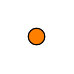
\begin{tikzpicture}
          \node [draw, fill=morange, circle, inner sep = 0, minimum size = 6] at (0, 0) {};
        \end{tikzpicture}
      \end{center}
      for each simple root $\alpha_{(i)} \in \Phi_S$.
    \item We join the nodes corresponding to $\alpha_{(i)}, \alpha_{(j)}$, with
      \[
        \max\{|A^{ij}|, |A^{ji}|\}
      \]
      many lines.
    \item If the roots have different lengths, we draw an arrow from the longer root to the shorter root. This happens when $A^{ij} \not= A^{ji}$.
  \end{enumerate}
\end{defi}
Note that we wouldn't have to draw too many lines. We have
\[
  A^{ij} = \frac{2|\alpha_{(i)}|}{|\alpha_{(j)}|} \cos \varphi_{ij},\quad A^{ji} = \frac{2|\alpha_{(j)}|}{|\alpha_{(i)}|} \cos \varphi_{ij},
\]
where $\varphi_{ij}$ is the angle between them. So we have
\[
  \cos^2 \varphi_{ij} = \frac{1}{4} A^{ij} A^{ji}.
\]
But we know $\cos^2 \varphi_{ij} \in [0, 1]$. So we must have
\[
  A^{ij} A^{ji} \in \{0, 1, 2, 3\}.
\]
So we have to draw at most $3$ lines, which isn't that bad. Moreover, we have the following information:
\begin{prop}
  A simple Lie algebra has roots of at most $2$ distinct lengths.
\end{prop}

\begin{proof}
  See example sheet.
\end{proof}

It is an exercise to see that all the information about $A^{ji}$ can be found from the Dynkin diagram.

We can now revisit the case of a rank 2 simple Lie algebra.
\begin{eg}
  The Cartan matrices of rank $2$ are given by
  \[
    \begin{pmatrix}
      2 & -1\\
      -1 & 2\\
    \end{pmatrix},\quad
    \begin{pmatrix}
      2 & -2\\
      -1 & 2
    \end{pmatrix},\quad
    \begin{pmatrix}
      2 & -3\\
      -1 & 2
    \end{pmatrix}
  \]
  These correspond to the Dynkin diagrams
  \begin{center}
    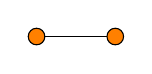
\begin{tikzpicture}
      \draw (3, 0) -- (4, 0);
      \foreach \x in {3,4} {
        \node [draw, fill=morange, circle, inner sep = 0, minimum size = 6] at (\x, 0) {};
      }
    \end{tikzpicture}
    \quad
    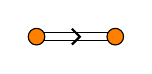
\begin{tikzpicture}
      \draw (0, 0.05) -- (1, 0.05);
      \draw (0, -0.05) -- (1, -0.05);

      \draw [thick] (0.45, 0.1) -- (0.55, 0) -- (0.45, -0.1);

      \foreach \x in {0,1} {
        \node [draw, fill=morange, circle, inner sep = 0, minimum size = 6] at (\x, 0) {};
      }
    \end{tikzpicture}
    \quad
    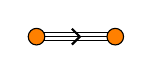
\begin{tikzpicture}
      \draw (0, 0.05) -- (1, 0.05);
      \draw (0, 0) -- (1, 0);
      \draw (0, -0.05) -- (1, -0.05);

      \draw [thick] (0.45, 0.1) -- (0.55, 0) -- (0.45, -0.1);

      \foreach \x in {0,1} {
        \node [draw, fill=morange, circle, inner sep = 0, minimum size = 6] at (\x, 0) {};
      }
    \end{tikzpicture}
  \end{center}
\end{eg}

The conditions on the matrices $A^{ij}$ now translate to conditions on the Dynkin diagrams which we will not write out, and it turns out we can classify all the allowed Dynkin diagrams as follows:
\begin{thm}[Cartan classification]
  The possible Dynkin diagrams include the following infinite families (where $n$ is the number of vertices):
  \begin{center}
    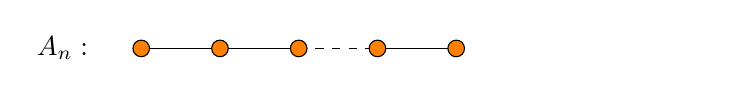
\begin{tikzpicture}
      \node at (-1, 0) {$A_n:$};
      \draw (0, 0) -- (2, 0);
      \draw [dashed] (2, 0) -- (3, 0);
      \draw (3, 0) -- (4, 0);
      \foreach \x in {0,1,2,3,4} {
        \node [draw, fill=morange, circle, inner sep = 0, minimum size = 6] at (\x, 0) {};
      }
      \node at (7, 0) {};
    \end{tikzpicture}
  \end{center}
  \begin{center}
    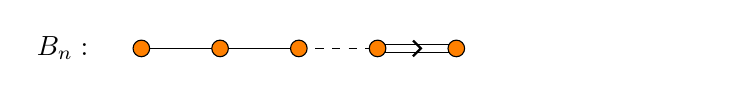
\begin{tikzpicture}
      \node at (-1, 0) {$B_n:$};
      \draw (0, 0) -- (2, 0);
      \draw [dashed] (2, 0) -- (3, 0);
      \draw (3, 0.05) -- (4, 0.05);
      \draw (3, -0.05) -- (4, -0.05);

      \draw [thick] (3.45, 0.1) -- (3.55, 0) -- (3.45, -0.1);

      \foreach \x in {0,1,2,3,4} {
        \node [draw, fill=morange, circle, inner sep = 0, minimum size = 6] at (\x, 0) {};
      }
      \node at (7, 0) {};
    \end{tikzpicture}
  \end{center}
  \begin{center}
    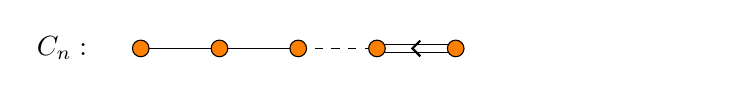
\begin{tikzpicture}
      \node at (-1, 0) {$C_n:$};
      \draw (0, 0) -- (2, 0);
      \draw [dashed] (2, 0) -- (3, 0);
      \draw (3, 0.05) -- (4, 0.05);
      \draw (3, -0.05) -- (4, -0.05);

      \draw [thick] (3.55, 0.1) -- (3.45, 0) -- (3.55, -0.1);

      \foreach \x in {0,1,2,3,4} {
        \node [draw, fill=morange, circle, inner sep = 0, minimum size = 6] at (\x, 0) {};
      }
      \node at (7, 0) {};
    \end{tikzpicture}
  \end{center}
  \begin{center}
    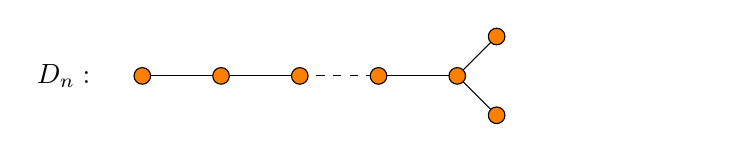
\begin{tikzpicture}
      \node at (-1, 0) {$D_n:$};
      \draw (0, 0) -- (2, 0);
      \draw [dashed] (2, 0) -- (3, 0);
      \draw (3, 0) -- (4, 0);
      \draw (4.5, 0.5) -- (4, 0) -- (4.5, -0.5);

      \foreach \x in {0,1,2,3,4} {
        \node [draw, fill=morange, circle, inner sep = 0, minimum size = 6] at (\x, 0) {};
      }
      \node [draw, fill=morange, circle, inner sep = 0, minimum size = 6] at (4.5, 0.5) {};
      \node [draw, fill=morange, circle, inner sep = 0, minimum size = 6] at (4.5, -0.5) {};
      \node at (7, 0) {};
    \end{tikzpicture}
  \end{center}
  And there are also five exceptional cases:
  \begin{center}
    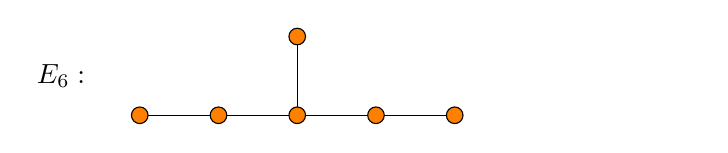
\begin{tikzpicture}
      \node at (-1, 0.5) {$E_6:$};
      \draw (0, 0) -- (4, 0);
      \draw (2, 0) -- (2, 1);
      \foreach \x in {0,1,2,3,4} {
        \node [draw, fill=morange, circle, inner sep = 0, minimum size = 6] at (\x, 0) {};
      }
      \node [draw, fill=morange, circle, inner sep = 0, minimum size = 6] at (2, 1) {};
      \node at (7, 0) {};
    \end{tikzpicture}
  \end{center}
  \begin{center}
    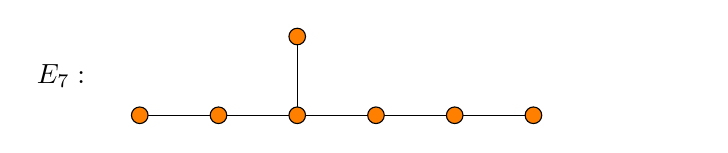
\begin{tikzpicture}
      \node at (-1, 0.5) {$E_7:$};
      \draw (0, 0) -- (5, 0);
      \draw (2, 0) -- (2, 1);
      \foreach \x in {0,1,2,3,4,5} {
        \node [draw, fill=morange, circle, inner sep = 0, minimum size = 6] at (\x, 0) {};
      }
      \node [draw, fill=morange, circle, inner sep = 0, minimum size = 6] at (2, 1) {};
      \node at (7, 0) {};
    \end{tikzpicture}
  \end{center}
  \begin{center}
    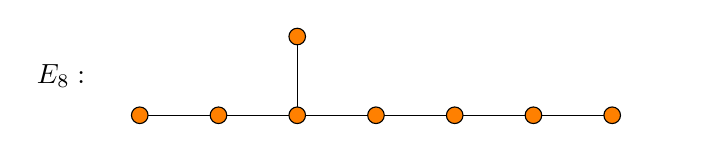
\begin{tikzpicture}
      \node at (-1, 0.5) {$E_8:$};
      \draw (0, 0) -- (6, 0);
      \draw (2, 0) -- (2, 1);
      \foreach \x in {0,1,2,3,4,5,6} {
        \node [draw, fill=morange, circle, inner sep = 0, minimum size = 6] at (\x, 0) {};
      }
      \node [draw, fill=morange, circle, inner sep = 0, minimum size = 6] at (2, 1) {};
      \node at (7, 0) {};
    \end{tikzpicture}
  \end{center}
  \begin{center}
    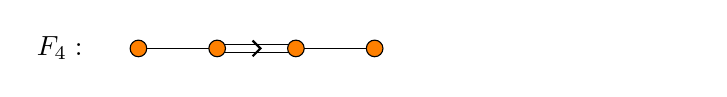
\begin{tikzpicture}
      \node at (-1, 0) {$F_4:$};
      \draw (0, 0) -- (1, 0);
      \draw (2, 0) -- (3, 0);

      \draw (1, 0.05) -- (2, 0.05);
      \draw (1, -0.05) -- (2, -0.05);

      \draw [thick] (1.45, 0.1) -- (1.55, 0) -- (1.45, -0.1);

      \foreach \x in {0,1,2,3} {
        \node [draw, fill=morange, circle, inner sep = 0, minimum size = 6] at (\x, 0) {};
      }
      \node at (7, 0) {};
    \end{tikzpicture}
  \end{center}
  \begin{center}
    \begin{tikzpicture}
      \node at (-1, 0) {$G_2:$};
      \draw (0, 0.05) -- (1, 0.05);
      \draw (0, 0) -- (1, 0);
      \draw (0, -0.05) -- (1, -0.05);

      \draw [thick] (0.45, 0.1) -- (0.55, 0) -- (0.45, -0.1);

      \foreach \x in {0,1} {
        \node [draw, fill=morange, circle, inner sep = 0, minimum size = 6] at (\x, 0) {};
      }
      \node at (7, 0) {};
    \end{tikzpicture}
  \end{center}
\end{thm}

\begin{eg}
  The infinite families $A_n, B_n, C_n, D_n$ correspond to well-known complex Lie groups by
  \begin{center}
    \begin{tabular}{cc}
      \toprule
      Family & Lie Group\\
      \midrule
      $A_n$ & $\mathcal{L}_\C(\SU(n + 1))$\\
      $B_n$ & $\mathcal{L}_\C(\SO(2n + 1))$\\
      $C_n$ & $\mathcal{L}_\C (\Sp(2n))$\\
      $D_n$ & $\mathcal{L}_\C (\SO(2n))$\\
      \bottomrule
    \end{tabular}
  \end{center}
  where the $\Sp(2n)$ are the \term{symplectic matrices}.
\end{eg}

Note that there is some repetition in our list. For example, we have $A_1 = B_1 = C_1 = D_1$ and $B_2 = C_2$. Also, $D_2$ does not give a simple Lie algebra, since it is disconnected. We have $D_2 \cong A_1 \oplus A_1$. So we have
\[
  \mathcal{L}_\C(\SO(4)) \cong \mathcal{L}_\C(\SU(2)) \oplus \mathcal{L}_\C(\SU(2)).
\]
Finally, we also have $D_3 = A_3$, and this reflects an isomorphism
\[
  \mathcal{L}_\C(\SU(4)) \cong \mathcal{L}_\C(\SO(6)).
\]
Hence, a list without repetitions is given by
\begin{center}
  \begin{tabular}{cl}
    $A_n$ & for $n\geq 1$,\\
    $B_n$ & for $n\geq 2$,\\
    $C_n$ & for $n\geq 3$,\\
    $D_n$ & for $n\geq 4$.
  \end{tabular}
\end{center}

This classification is very important in modern theoretical physics, since in many theories, we need to pick a Lie group as, say, our gauge group. So knowing what Lie groups are around lets us know what theories we can have.

\subsection{Reconstruction}
Now given the Cartan matrix, we want to reconstruct the Lie algebra itself.

Recall that we had a Cartan-Weyl basis
\[
  \{H^i, E^\alpha: i = 1, \cdots, r: \alpha \in \Phi\}.
\]
The first thing to do in the reconstruction is to figure out what the set of roots is.

By definition, the Cartan matrix determines simple roots $\alpha_{(i)}$ for $i = 1, \cdots, r$. We can read off the inner products from the Cartan matrix as
\[
  A^{ij} = \frac{2(\alpha_{(i)}, \alpha_{(j)})}{(\alpha_{(j)}, \alpha_{(j)})} = \frac{2|\alpha_{(i)}|}{|\alpha_{(j)}|} \cos \varphi_{ij}.
\]
This allows us to find the simple roots.

How about the other roots? We can find them by considering the root strings, as we know that the length of the $\alpha_{(i)}$-string through $\alpha_{(j)}$ is given by
\[
  \ell_{ij} = 1 - A_{ji} \in \N.
\]
So we can work out the length of the root string from each simple root. By Cartan's theorem, this gives us all roots.

Instead of going through a formal and general reconstruction, we do an example.

\begin{eg}
  Consider $\mathfrak{g} = A_2$. We have a Dynkin diagram
  \begin{center}
    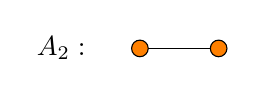
\begin{tikzpicture}
      \node at (-1, 0) {$A_2:$};
      \draw (0, 0) -- (1, 0);
      \foreach \x in {0,1} {
        \node [draw, fill=morange, circle, inner sep = 0, minimum size = 6] at (\x, 0) {};
      }
    \end{tikzpicture}
  \end{center}
  So we see that the Cartan matrix is
  \[
    A =
    \begin{pmatrix}
      2 & -1\\
      -1 & 2
    \end{pmatrix}.
  \]
  So we know that $\mathfrak{g}$ has two simple roots $\alpha, \beta \in \Phi$, and we know
  \[
    A_{12} = A_{21} = \frac{2(\alpha, \beta)}{(\alpha, \alpha)} = \frac{2(\beta, \alpha)}{(\beta, \beta)} = -1.
  \]
  So we find that $(\alpha, \alpha) = (\beta, \beta)$, and $\varphi_{\alpha\beta} = \frac{2\pi}{3}$. So we can display the roots as
  \begin{center}
    \begin{tikzpicture}
      \draw [->] (0, 0) -- (2, 0) node [right] {$\alpha$};
      \draw [->] (0, 0) -- (-1, 1.732) node [above] {$\beta$};
      \draw (0.6, 0) arc(0:120:0.6) node [pos=0.5, anchor=south west] {$\frac{2\pi}{3}$};
    \end{tikzpicture}
  \end{center}
  Since $\alpha, \beta \in \Phi_S$, we know $\pm(\alpha - \beta) \not\in \Phi$, and also we have
  \[
    \ell_{\alpha, \beta} = \ell_{\beta, \alpha} = 1 - \frac{2 (\alpha, \beta)}{(\alpha, \alpha)} = 2.
  \]
  So we have roots $\beta + n \alpha, \alpha + \tilde{n}\beta$ for $n, \tilde{n} \in \{0, 1\}$. So in fact our list of roots contains
  \[
    \alpha, \beta, \alpha + \beta \in \Phi.
  \]
  These are the positive ones. We know each of these roots has a negative counterpart. So we have more roots
  \[
    -\alpha, -\beta, -\alpha - \beta \in \Phi.
  \]
  Then by our theorem, we know these are all the roots. We can find the length of $\alpha + \beta$ by
  \begin{align*}
    (\alpha + \beta, \alpha + \beta) &= (\alpha, \alpha) + (\beta, \beta) + 2(\alpha, \beta)\\
    &= (\alpha, \alpha) + (\beta, \beta) - (\beta, \beta)\\
    &= (\alpha, \alpha).
  \end{align*}
  So in fact all roots have the same length. So if we draw all our roots, we get
  \begin{center}
    \begin{tikzpicture}
      \draw [->] (0, 0) -- (2, 0) node [right] {$\alpha$};
      \draw [->] (0, 0) -- (-1, 1.732) node [above] {$\beta$};
      \draw [->] (0, 0) -- (1, 1.732) node [right] {$\alpha + \beta$};
      \draw [->] (0, 0) -- (-2, 0) node [left] {$-\alpha$};
      \draw [->] (0, 0) -- (1, -1.732) node [below] {$-\beta$};
      \draw [->] (0, 0) -- (-1, -1.732) node [below] {$-\alpha - \beta$};
    \end{tikzpicture}
  \end{center}
  So the Cartan-Weyl basis consists of
  \[
    \mathcal{B}_{\mathrm{CW}} = \{H^1, H^2, E^{\pm \alpha}, E^{\pm \beta}, E^{\pm(\alpha + \beta)}\}.
  \]
  This is the complete Cartan-Weyl basis of $A_2$. So this has dimension $2 + 6 = 8$.

  If we want to find out the brackets of these things, we look at the ones we have previously written down, and use the Jacobi identity many times.
\end{eg}

\section{Representation of Lie algebras}
We now try to understand the possible representations of Lie algebras. It turns out they again are pretty restricted.

\subsection{Weights}
Let $\rho$ be a representation of $\mathfrak{g}$ on $V$. Then it is completely determined by the images
\begin{align*}
  H^i &\mapsto \rho(H^i) \in \gl(V)\\
  E^\alpha &\mapsto \rho(E^\alpha) \in \gl(V).
\end{align*}
Again, we know that
\[
  [\rho(H^i), \rho(H^j)] = \rho([H^i, H^j]) = 0.
\]
So all $\rho(H^i)$ commute, and by linear algebra, we know they have a common eigenvector $v_\lambda$. Again, for each $H \in \mathfrak{h}$, we know
\[
  \rho(H) v_\lambda = \lambda(H) v_\lambda
\]
for some $\lambda(H)$, and $\lambda$ lives in $\mathfrak{h}^*$.
\begin{defi}[Weight of representation]\index{weight of representation}\index{representation!weight}
  Let $\rho: \mathfrak{g} \to \gl(V)$ be a representation of $\mathfrak{g}$. Then if $v_\lambda \in V$ is an eigenvector of $\rho(H)$ for all $H \in \mathfrak{h}$, we say $\lambda\in \mathfrak{h}^*$ is a \emph{weight} of $\rho$, where
  \[
    \rho(H) v_\lambda = \lambda(H) v_\lambda
  \]
  for all $H \in \mathfrak{h}$.

  The \emph{weight set} $S_\rho$ of $\rho$ is the set of all weights.
\end{defi}
For a weight $\lambda$, we write $V_\lambda$ for the subspace that consists of vectors $v$ such that
\[
  \rho(H) v = \lambda(H) v.
\]
Note that the weights can have multiplicity, i.e.\ $V_\lambda$ need not be $1$-dimensional. We write
\[
  m_\lambda = \dim V_\lambda \geq 1
\]
for the \term{multiplicity} of the weight.

\begin{eg}
  By definition, we have
  \[
    [H^i, E^\alpha] = \alpha^i E^\alpha
  \]
  So we have
  \[
    \ad_{H^i} E^\alpha = \alpha^i E_\alpha.
  \]
  In terms of the adjoint representation, this says
  \[
    \rho_{\mathrm{adj}} (H^i) E_\alpha = \alpha^i E_\alpha.
  \]
  So the roots $\alpha$ are the weights of the adjoint representation.
\end{eg}
Recall that for $\su_\C(2)$, we know that the weights are always integers. This will be the case in general as well.

Given any representation $\rho$, we know it has at least one weight $\lambda$ with an eigenvector $v \in V_\lambda$. We'll see what happens when we apply the step operators $\rho(E^\alpha)$ to it, for $\alpha \in \Phi$. We have
\[
  \rho(H^i) \rho(E^\alpha)v = \rho(E^\alpha) \rho(H^i) v + [\rho(H^i), \rho(E^\alpha)] v.
\]
We know that
\[
  [\rho(H^i), \rho(E^\alpha)] = \rho([H^i, E^\alpha]) = \alpha^i \rho(E^\alpha).
\]
So we know that if $v \in V_\lambda$, then
\[
  \rho(H^i)\rho(E^\alpha)v = (\lambda^i + \alpha^i) \rho(E^\alpha) v.
\]
So the weight of the vector has been shifted by $\alpha$. Thus, for all vectors $v \in V_\lambda$, we find that
\[
  \rho(E^\alpha) v \in V_{\lambda + \alpha}.
\]
However, we do not know a priori if $V_{\lambda + \alpha}$ is a thing at all. If $V_{\lambda + \alpha} = \{0\}$, i.e.\ $\lambda + \alpha$ is not a weight, then we know that $\rho(E^\alpha) v = 0$.

So the Cartan elements $H^i$ preserve the weights, and the step operators $E^\alpha$ increment the weights by $\alpha$.

Consider the action of our favorite $\su(2)_\alpha$ subalgebra on the representation space. In other words, we consider the action of $\{\rho(h^\alpha), \rho(e^\alpha), \rho(e^{-\alpha})\}$ on $V$. Then $V$ becomes the representation space for some representation $\rho_\alpha$ for $\su(2)_\alpha$.

Now we can use what we know about the representations of $\su(2)$ to get something interesting about $V$. Recall that we defined
\[
  h^\alpha = \frac{2}{(\alpha, \alpha)} H^\alpha = \frac{2}{(\alpha, \alpha)} (\kappa^{-1})_{ij} \alpha^j H^i.
\]
So for any $v \in V_\lambda$, after some lines of algebra, we find that
\[
  \rho(h^\alpha)(v) = \frac{2(\alpha, \lambda)}{(\alpha, \alpha)} v.
\]
So we know that we must have
\[
  \frac{2(\alpha, \lambda)}{(\alpha, \alpha)} \in \Z
\]
for all $\lambda \in S_\rho$ and $\alpha \in \Phi$. So in particular, we know that $(\alpha_{(i)}, \lambda) \in \R$ for all simple roots $\alpha_{(i)}$. In particular, it follows that $\lambda \in \mathfrak{h}^*_\R$ (if we write $\lambda$ as a sum of the $\alpha_{(i)}$, then the coefficients are the unique solution to a real system of equations, hence are real).

Again, from these calculations, we see that $\bigoplus_{\lambda \in S_\rho} V_\lambda$ is a subrepresentation of $V$, so by irreducibility, everything is a linear combination of these simultaneous eigenvectors, i.e.\ we must have
\[
  V = \bigoplus_{\lambda \in S_\rho} V_\lambda.
\]
In particular, this means all $\rho(H)$ are diagonalizable for $H \in \mathfrak{h}$.

\subsection{Root and weight lattices}
Recall that the simple roots are a basis for the whole root space. In particular, any positive root can be written as a positive sum of simple roots. So for any $\beta \in \Phi$, we can write
\[
  \beta = \sum_{i = 1}^r \beta^i \alpha_{(i)},
\]
where $\beta^i \in \Z$ for $i = 1, \cdots, r$. Hence all roots lie in a \emph{root lattice}:
\begin{defi}[Root lattice]\index{root lattice}
  Let $\mathfrak{g}$ be a Lie algebra with simple roots $\alpha_{(i)}$. Then the \emph{root lattice} is defined as
  \[
    \mathcal{L}[\mathfrak{g}] = \spn_\Z\{\alpha_{(i)}: i = 1, \cdots, r\}.
  \]
\end{defi}
Note that here we are taking the integer span, not the real span.

What we want to do is to define an analogous \emph{weight lattice}, where all possible weights lie.

We start by defining some funny normalization of the roots:
\begin{defi}[Simple co-root]\index{simple co-root}\index{co-root}
  The \emph{simple co-roots} are
  \[
    \check{\alpha}_{(i)} = \frac{2 \alpha_{(i)}}{(\alpha_{(i)},\alpha_{(i)})}.
  \]
\end{defi}
Similarly, we can define the co-root lattice:

\begin{defi}[Co-root lattice]\index{co-root lattice}
  Let $\mathfrak{g}$ be a Lie algebra with simple roots $\alpha_{(i)}$. Then the \emph{co-root lattice} is defined as
  \[
    \check{\mathcal{L}}[\mathfrak{g}] = \spn_\Z\{\check\alpha_{(i)}: i = 1, \cdots, r\}.
  \]
\end{defi}

\begin{defi}[Weight lattice]\index{weight lattice}
  The \emph{weight lattice} $\mathcal{L}_W[\mathfrak{g}]$ is the \emph{dual} to the co-root lattice:
  \[
    \mathcal{L}_W [\mathfrak{g}] = \check{\mathcal{L}}^*[\mathfrak{g}] = \{\lambda \in \mathfrak{h}^*_\R: (\lambda, \mu) \in \Z \text{ for all }\mu \in \check{\mathcal{L}}[\mathfrak{g}]\}.
  \]
\end{defi}
So we know $\lambda \in \mathcal{L}_W[\mathfrak{g}]$ iff for all $\alpha_{(i)}$, we have
\[
  (\lambda , \check{\alpha}_{(i)}) = \frac{2(\alpha_{(i)}, \lambda)}{(\alpha_{(i)}, \alpha_{(i)})} \in \Z.
\]
So by what we have previously computed, we know that all weights $\lambda \in S_\rho$ are in $\mathcal{L}_W [\mathfrak{g}]$.

Given the basis
\[
  \mathcal{B} = \{\check{\alpha}_{(i)}: i = 1, \cdots, r\}
\]
for $\check{\mathcal{L}}[\mathfrak{g}]$, we define the dual basis
\[
  \mathcal{B}^* = \{\omega_{(i)} : i = 1, \cdots, r\}
\]
by demanding
\[
  (\check{\alpha}_{(i)}, \omega_{(j)}) = \frac{2(\alpha_{(i)}, \omega_{(j)})}{(\alpha_{(i)}, \alpha_{(i)})} = \delta_{ij}.
\]
These $\omega_{(i)}$ are known as the \term{fundamental weights}. As the simple roots span $\mathfrak{h}^*_\R$, we can write
\[
  \omega_{(i)} = \sum_{j = 1}^r B_{ij} \alpha_{(j)}
\]
for some $B_{ij} \in \R$. Plugging this into the definition, we find
\[
  \sum_{k = 1}^r \frac{2(\alpha_{(i)}, \alpha_{(k)})}{(\alpha_{(i)}, \alpha_{(i)})} B_{jk} = \delta^i_j.
\]
So we know
\[
  \sum_{k = 1}^r B_{jk}A^{ki} = \delta^i_j,
\]
i.e.\ $B$ is the inverse of the Cartan matrix $A$. Thus we can write
\[
  \alpha_{(i)} = \sum_{j = 1}^r A^{ij} \omega_{(j)}.
\]
\begin{eg}
  Consider $\mathfrak{g} = A_2$. Then we have
  \[
    A =
    \begin{pmatrix}
      2 & -1\\
      -1 & 2
    \end{pmatrix}.
  \]
  Then we have
  \begin{align*}
    \alpha &= \alpha_{(1)} = 2 \omega_{(1)} - \omega_{(2)}\\
    \beta &= \alpha_{(2)} = - \omega_{(1)} + 2 \omega_{(2)}.
  \end{align*}
  So we have
  \begin{align*}
    \omega_{(1)} &= \frac{1}{3} (2 \alpha + \beta)\\
    \omega_{(2)} &= \frac{1}{3} (\alpha + 2 \beta).
  \end{align*}
  We can then draw the weight lattice:
  \begin{center}
    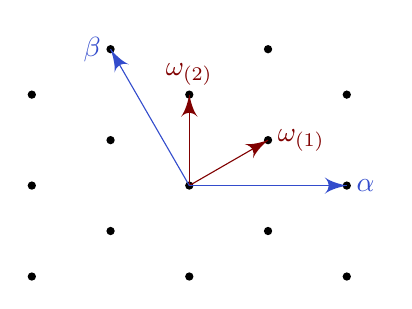
\begin{tikzpicture}
      \foreach \x in {-2, 0, 2} {
        \foreach \y in {0, 1.155, -1.155} {
          \node [circ] at (\x, \y) {};
        }
      }
      \foreach \x in {-1, 1} {
        \foreach \y in {0.577, -0.577, 1.732} {
          \node [circ] at (\x, \y) {};
        }
      }
      \draw [mred, ->] (0, 0) -- (0, 1.155) node [above] {$\omega_{(2)}$};
      \draw [mred, ->] (0, 0) -- (1, 0.577) node [right] {$\omega_{(1)}$};
      \draw [mblue, ->] (0, 0) -- (2, 0) node [right] {$\alpha$};
      \draw [mblue, ->] (0, 0) -- (-1, 1.732) node [left] {$\beta$};
    \end{tikzpicture}
  \end{center}
  Note that the roots are also in the weight lattice, because they are weights of the adjoint representation.
\end{eg}

Given any weight $\lambda \in S_\rho \subseteq \mathcal{L}_W[\mathfrak{g}]$, we can write
\[
  \lambda = \sum_{i = 1}^r \lambda^i \omega_{(i)}
\]
for some $\lambda^i \in \Z$. These $\{\lambda^i\}$ are called \term{Dynkin labels} of the weight $\lambda$.

%What do these coefficients tell us?
%\begin{prop}
% Suppose $v_\lambda$ has weight
% \[
% \lambda = \sum_{i = 1}^r \lambda^i \omega_{(i)}.
% \]
% Then $\lambda(h^i) = \lambda^i$, i.e.
% \[
% \rho(h^i) v_\lambda = \lambda^i v_\lambda.
% \]
%\end{prop}
%
%\begin{proof}
% What we want to show is exactly that
% \[
% \omega_{(i)}(h^j) = \delta_i^j.
% \]
% In other words, we need
% \[
% \omega_{(i)} (h^\alpha) = (\check{\alpha}, \omega_{(i)}).
% \]
%\end{proof}
\subsection{Classification of representations}
Suppose we have a representation $\rho$ of $\mathfrak{g}$. We can start with any eigenvector $v \in V_\lambda$. We then keep applying things of the form $\rho(E^\alpha)$, where $\alpha \in \Phi_+$ is a \emph{positive} weight. Doing so will bring us further away from the hyperplane dividing the positive and negative weights, and since there are only finitely many weights, we must eventually stop. This is known as a \emph{highest weight}.

\begin{defi}[Highest weight]\index{highest weight}
  A \emph{highest weight} of a representation $\rho$ is a weight $\Lambda \in S_\rho$ whose associated eigenvector $v_\Lambda$ is such that
  \[
    \rho(E^\alpha) v_\Lambda = 0
  \]
  for all $\alpha \in \Phi_+$.
\end{defi}
The \emph{Dynkin labels} (or \emph{indices}) of a representation are the Dynkin labels of its highest weight.

Now if $v \in V_\lambda$, then we know
\[
  \rho(E^\alpha) v \in V_{\lambda + \alpha},
\]
if $\lambda + \alpha \in S_\rho$ (and vanishes otherwise). So acting with the step operators translates us in the weight lattice by the vector corresponding to the root.

In the case of $\su(2)$, we found out an explicit formula for when this will stop. In this general case, we have the following result which we will not prove:

\begin{thm}
  For any finite-dimensional representation of $\mathfrak{g}$, if
  \[
    \lambda = \sum_{i = 1}^r \lambda^i \omega_{(i)} \in S_\rho,
  \]
  then we know
  \[
    \lambda - m_{(i)} \alpha_{(i)} \in S_\rho,
  \]
  for all $m_{(i)} \in \Z$ and $0 \leq m_{(i)} \leq \lambda^i$.

  If we know further that $\rho$ is irreducible, then we can in fact obtain all weights by starting at the highest weight and applying this procedure.

  Moreover, for any
  \[
    \Lambda = \sum \Lambda^i \omega_{(i)} \in \mathcal{L}_W[\mathfrak{g}],
  \]
  this is the highest weight of some irreducible representation if and only if $\Lambda^i \geq 0$ for all $i$.
\end{thm}

This gives us a very concrete way of finding, at least the weights, of an irreducible representation. In general, though, we don't immediately know the multiplicities of the weights.

\begin{defi}[Dominant integral weight]\index{dominant integral weight}
  A \emph{dominant integral weight} is a weight
  \[
    \Lambda = \sum \Lambda^i \omega_{(i)} \in \mathcal{L}_W[\mathfrak{g}],
  \]
  such that $\Lambda^i \geq 0$ for all $i$.
\end{defi}

\begin{eg}
  Take the example of $\mathfrak{g} = A_2$. It is a fact that the \emph{fundamental representation} $f$ has Dynkin labels $(1, 0)$. In other words,
  \[
    \Lambda = \omega_{(1)}.
  \]
  To get the remaining weights, we subtract roots:
  \begin{enumerate}
    \item $\Lambda = \omega_{(1)} \in S_f$. So we can subtract by $\alpha_{(1)}$ exactly once.
    \item So
      \begin{align*}
        \lambda &= \omega_{(1)} - (2 \omega_{(1)} - \omega_{(2)}) \\
        &= - \omega_{(1)} + \omega_{(2)} \in S_f.
      \end{align*}
      This has Dynkin labels $(-1, 1)$. So we can do one further subtraction to get a new weight
      \begin{align*}
        \lambda - \alpha_{(2)} &= - \omega_{(1)} + \omega_{(2)} - (2 \omega_{(2)} - \omega_{(1)})\\
        &= -\omega_{(2)}
      \end{align*}
  \end{enumerate}
  In the weight diagram, these are given by
  \begin{center}
    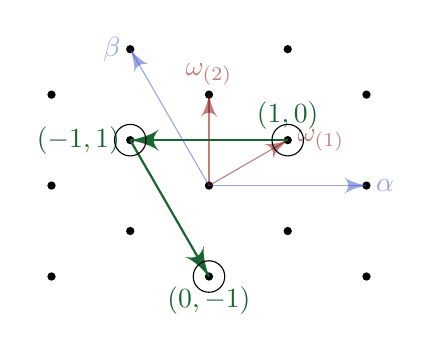
\begin{tikzpicture}
      \foreach \x in {-2, 0, 2} {
        \foreach \y in {0, 1.155, -1.155} {
          \node [circ] at (\x, \y) {};
        }
      }
      \foreach \x in {-1, 1} {
        \foreach \y in {0.577, -0.577, 1.732} {
          \node [circ] at (\x, \y) {};
        }
      }
      \draw [opacity=0.5, mred, ->] (0, 0) -- (0, 1.155) node [above] {$\omega_{(2)}$};
      \draw [opacity=0.5, mred, ->] (0, 0) -- (1, 0.577) node [right] {$\omega_{(1)}$};
      \draw [opacity=0.5, mblue, ->] (0, 0) -- (2, 0) node [right] {$\alpha$};
      \draw [opacity=0.5, mblue, ->] (0, 0) -- (-1, 1.732) node [left] {$\beta$};

      \draw [mgreen, thick, ->] (1, 0.577) node [above] {$(1, 0)$} -- (-1, 0.577);
      \draw [mgreen, thick, ->] (-1, 0.577) node [left] {$(-1, 1)$} -- (0, -1.155) node [below] {$(0, -1)$};

      \draw (0, -1.155) circle [radius=0.2];
      \draw (1, 0.577) circle [radius=0.2];
      \draw (-1, 0.577) circle [radius=0.2];
    \end{tikzpicture}
  \end{center}
  In general, for a dominant integral weight of the form
  \[
    \Lambda = \Lambda^1 \omega_{(1)} + \Lambda^2 \omega_{(2)} \in \mathcal{L}_W[A_2]
  \]
  for $\Lambda^1, \Lambda^2 \in \Z_{\geq 0}$. We then get an irrep $\rho_{(\Lambda^1, \Lambda^2)}$ of $A_2$.

  One can show, via characters, that the dimension of this representation is given by
  \[
    \dim \rho_{(\Lambda^1, \Lambda^2)} = \frac{1}{2} (\Lambda^1 + 1)(\Lambda^2 + 1)(\Lambda^1 + \Lambda^2 + 2).
  \]
  This is symmetric in $\Lambda^1$ and $\Lambda^2$. So if $\Lambda^1\not= \Lambda^2$, then we get a pair of distinct representations of the same dimension. It is a fact that
  \[
    \lambda \in S_{(\Lambda^1, \Lambda^2)} \Leftrightarrow -\lambda \in S_{(\Lambda^2, \Lambda^1)},
  \]
  and we have
  \[
    \rho_{(\Lambda_1, \Lambda_2)} = \bar{\rho}_{(\Lambda_2, \Lambda_1)}.
  \]
  On the other hand, if $\Lambda_1 = \Lambda_2$, then this representation is self-conjugate.

  The first few representations of $A_2$ are given by
  \begin{center}
    \begin{tabular}{ccc}
      \toprule
      Highest weight & Dimension & Name\\
      \midrule
      $\rho_{(0, 0)}$ & $\mathbf{1}$ & Trivial\\
      $\rho_{(1, 0)}$ & $\mathbf{3}$ & Fundamental\\
      $\rho_{(0, 1)}$ & $\bar{\mathbf{3}}$ & Anti-fundamental\\
      $\rho_{(2, 0)}$ & $\mathbf{6}$\\
      $\rho_{(0, 2)}$ & $\bar{\mathbf{6}}$\\
      $\rho_{(1, 1)}$ & $\mathbf{8}$ & Adjoint\\
      \bottomrule
    \end{tabular}
  \end{center}
  We can figure out the weights of the adjoint representation with $\Lambda = (1, 1) \in S_\rho$. Since both labels are positive, we can subtract both $\alpha_{(1)}$ and $\alpha_{(2)}$ to get
  \begin{align*}
    \Lambda - \alpha_{(1)} &= (-1, 2)\\
    \Lambda - \alpha_{(2)} &= (2, -1)
  \end{align*}
  \begin{center}
    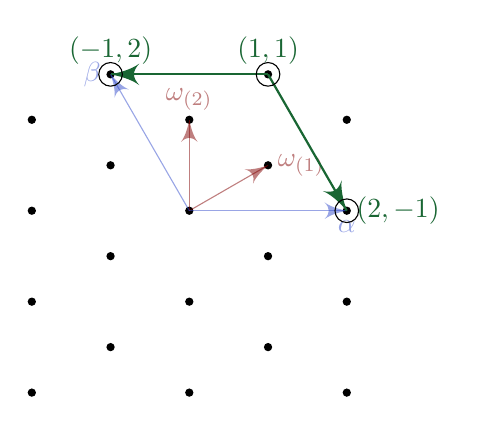
\begin{tikzpicture}
      \foreach \x in {-2, 0, 2} {
        \foreach \y in {0, 1.155, -1.155, -2.310} {
          \node [circ] at (\x, \y) {};
        }
      }
      \foreach \x in {-1, 1} {
        \foreach \y in {0.577, -0.577, 1.732, -1.732} {
          \node [circ] at (\x, \y) {};
        }
      }
      \draw [opacity=0.5, mred, ->] (0, 0) -- (0, 1.155) node [above] {$\omega_{(2)}$};
      \draw [opacity=0.5, mred, ->] (0, 0) -- (1, 0.577) node [right] {$\omega_{(1)}$};
      \draw [opacity=0.5, mblue, ->] (0, 0) -- (2, 0) node [below] {$\alpha$};
      \draw [opacity=0.5, mblue, ->] (0, 0) -- (-1, 1.732) node [left] {$\beta$};

      \draw [mgreen, thick, ->] (1, 1.732) -- (-1, 1.732);
      \draw [mgreen, thick, ->] (1, 1.732) -- (2, 0);

      \node [above, mgreen] at (1, 1.732) {$(1, 1)$};
      \node [above, mgreen] at (-1, 1.732) {$(-1, 2)$};
      \node [right, mgreen] at (2, 0) {$(2, -1)$};

      \draw (1, 1.732) circle [radius=0.15];
      \draw (2, 0) circle [radius=0.15];
      \draw (-1, 1.732) circle [radius=0.15];
    \end{tikzpicture}
  \end{center}
  Now we have a $+2$ in the Dynkin labels. So we can subtract twice. So we have the following weights:
  \begin{align*}
    \Lambda - \alpha_{(1)} - \alpha_{(2)} &= (0, 0) \\
    \Lambda - \alpha_{(1)} - 2\alpha_{(2)} &= (1, -2)\\
    \Lambda - 2\alpha_{(1)} - \alpha_{(2)} &= (-2, 1)
  \end{align*}
  \begin{center}
    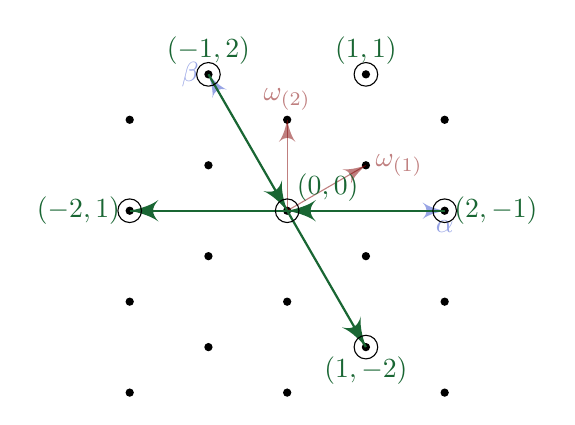
\begin{tikzpicture}
      \foreach \x in {-2, 0, 2} {
        \foreach \y in {0, 1.155, -1.155, -2.310} {
          \node [circ] at (\x, \y) {};
        }
      }
      \foreach \x in {-1, 1} {
        \foreach \y in {0.577, -0.577, 1.732, -1.732} {
          \node [circ] at (\x, \y) {};
        }
      }
      \draw [opacity=0.5, mred, ->] (0, 0) -- (0, 1.155) node [above] {$\omega_{(2)}$};
      \draw [opacity=0.5, mred, ->] (0, 0) -- (1, 0.577) node [right] {$\omega_{(1)}$};
      \draw [opacity=0.5, mblue, ->] (0, 0) -- (2, 0) node [below] {$\alpha$};
      \draw [opacity=0.5, mblue, ->] (0, 0) -- (-1, 1.732) node [left] {$\beta$};

      \draw [mgreen, thick, ->] (-1, 1.732) -- (0, 0);
      \draw [mgreen, thick, ->] (2, 0) -- (0, 0);
      \draw [mgreen, thick, ->] (0, 0) -- (-2, 0);
      \draw [mgreen, thick, ->] (0, 0) -- (1, -1.732);

      \node [above, mgreen] at (1, 1.732) {$(1, 1)$};
      \node [above, mgreen] at (-1, 1.732) {$(-1, 2)$};
      \node [right, mgreen] at (2, 0) {$(2, -1)$};
      \node [anchor = south west, mgreen] at (0, 0) {$(0, 0)$};
      \node [below, mgreen] at (1, -1.732) {$(1, -2)$};
      \node [left, mgreen] at (-2, 0) {$(-2, 1)$};

      \draw (1, 1.732) circle [radius=0.15];
      \draw (2, 0) circle [radius=0.15];
      \draw (-1, 1.732) circle [radius=0.15];
      \draw (-2, 0) circle [radius=0.15];
      \draw (1, -1.732) circle [radius=0.15];
      \draw (0, 0) circle [radius=0.15];
    \end{tikzpicture}
  \end{center}
  Finally, we can subtract $\alpha_{(1)}$ from the second or $\alpha_{(2)}$ from the third to get
  \[
    \Lambda - 2\alpha_{(1)} - 2 \alpha_{(2)} = (-1, -1) \in S_\rho.
  \]
  \begin{center}
    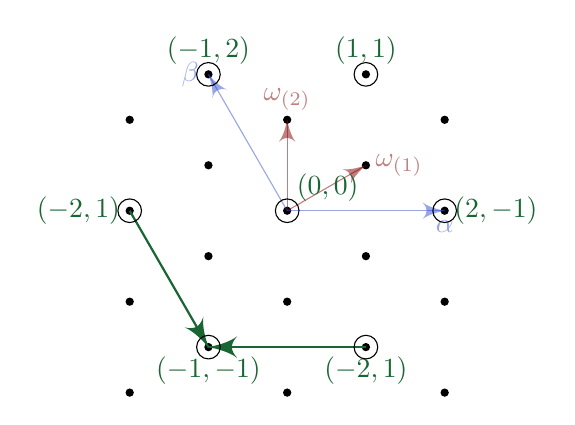
\begin{tikzpicture}
      \foreach \x in {-2, 0, 2} {
        \foreach \y in {0, 1.155, -1.155, -2.310} {
          \node [circ] at (\x, \y) {};
        }
      }
      \foreach \x in {-1, 1} {
        \foreach \y in {0.577, -0.577, 1.732, -1.732} {
          \node [circ] at (\x, \y) {};
        }
      }
      \draw [opacity=0.5, mred, ->] (0, 0) -- (0, 1.155) node [above] {$\omega_{(2)}$};
      \draw [opacity=0.5, mred, ->] (0, 0) -- (1, 0.577) node [right] {$\omega_{(1)}$};
      \draw [opacity=0.5, mblue, ->] (0, 0) -- (2, 0) node [below] {$\alpha$};
      \draw [opacity=0.5, mblue, ->] (0, 0) -- (-1, 1.732) node [left] {$\beta$};

      \draw [mgreen, thick, ->] (1, -1.732) -- (-1, -1.732);
      \draw [mgreen, thick, ->] (-2, 0) -- (-1, -1.732);

      \node [above, mgreen] at (1, 1.732) {$(1, 1)$};
      \node [above, mgreen] at (-1, 1.732) {$(-1, 2)$};
      \node [right, mgreen] at (2, 0) {$(2, -1)$};
      \node [anchor = south west, mgreen] at (0, 0) {$(0, 0)$};
      \node [below, mgreen] at (1, -1.732) {$(-2, 1)$};
      \node [left, mgreen] at (-2, 0) {$(-2, 1)$};
      \node [below, mgreen] at (-1, -1.732) {$(-1, -1)$};

      \draw (1, 1.732) circle [radius=0.15];
      \draw (2, 0) circle [radius=0.15];
      \draw (-1, 1.732) circle [radius=0.15];
      \draw (-1, -1.732) circle [radius=0.15];
      \draw (-2, 0) circle [radius=0.15];
      \draw (1, -1.732) circle [radius=0.15];
      \draw (0, 0) circle [radius=0.15];
    \end{tikzpicture}
  \end{center}
  Now notice that we only have seven weights, not eight. This is because our algorithm did not tell us the multiplicity of the weights. However, in this particular case, we know, because this is the adjoint representation, and the Cartan generators give us two things of weight $0$. So we can plot all weights with multiplicity as
  \begin{center}
    \begin{tikzpicture}
      \foreach \x in {-2, 0, 2} {
        \foreach \y in {0, 1.155, -1.155, -2.310} {
          \node [circ] at (\x, \y) {};
        }
      }
      \foreach \x in {-1, 1} {
        \foreach \y in {0.577, -0.577, 1.732, -1.732} {
          \node [circ] at (\x, \y) {};
        }
      }
      \draw (1, 1.732) circle [radius=0.15];
      \draw (2, 0) circle [radius=0.15];
      \draw (-1, 1.732) circle [radius=0.15];
      \draw (-1, -1.732) circle [radius=0.15];
      \draw (-2, 0) circle [radius=0.15];
      \draw (1, -1.732) circle [radius=0.15];
      \draw (0, 0) circle [radius=0.15];
      \draw (0, 0) circle [radius=0.25];
    \end{tikzpicture}
  \end{center}
\end{eg}

It is a general fact that the weight lattice traces out a polygon like this, and the vertices at the perimeter are always non-degenerate. So in this case, we could also have figured out the multiplicty by using this general fact.

\subsection{Decomposition of tensor products}
The last thing we need to know how to do is how we can decompose tensor products of irreps. This is not hard. It is just what we did for $\su(2)$ but in a more general context.

We let $\rho_\Lambda$ and $\rho_{\Lambda'}$ be irreps of $\mathfrak{g}$ with corresponding representation spaces $V_\Lambda$ and $V_{\Lambda'}'$. Then we can write
\[
  V_\Lambda = \bigoplus_{\lambda \in S_\Lambda} V_\lambda,\quad V_{\Lambda'}' = \bigoplus_{\lambda' \in S_{\Lambda'}} V'_{\lambda'}.
\]
If $v_\lambda \in V_\Lambda$ and $v_{\lambda'} \in V_{\Lambda'}'$, then for $H \in \mathfrak{h}$, we have
\begin{align*}
  (\rho_\Lambda \otimes \rho_{\Lambda'})(H)(v_\lambda \otimes v_{\lambda'}) &= \rho_\Lambda(H)v_\lambda \otimes v_{\lambda'} + v_\lambda \otimes \rho_{\Lambda'}(H) v_{\lambda'}\\
  &= \lambda(H) v_\lambda \otimes v_{\lambda'} + \lambda'(H) v_\lambda \otimes v_{\lambda'}\\
  &= (\lambda + \lambda')(H) v_\lambda \otimes v_{\lambda'}.
\end{align*}
Since things of the form $v_\lambda \otimes v_{\lambda'}$ span $V_\Lambda \otimes V_{\Lambda'}$, we know
\[
  S_{\Lambda \otimes \Lambda'} = \{\lambda + \lambda': \lambda \in S_\Lambda, \lambda' \in S_{\Lambda'}\}
\]
with multiplicities. To figure out the decomposition, we find out what the highest weight of the tensor product is, and then subtract off the factors corresponding to the highest weight, and then repeat.
\begin{eg}
  Consider $\mathfrak{g} = A_2$, and the fundamental representation $\rho_{(1, 0)}$. We consider
  \[
    \rho_{(1, 0)} \otimes \rho_{(1, 0)}.
  \]
  Recall that the weight set is given by
  \[
    S_{(1, 0)} = \{\omega_{(1)}, -\omega_{(1)} + \omega_{(2)}, -\omega_{(2)}\}.
  \]
  We can then draw the collection of all weights in $\rho_{(1, 0)} \otimes \rho_{(1, 0)}$ as follows:
  \begin{center}
    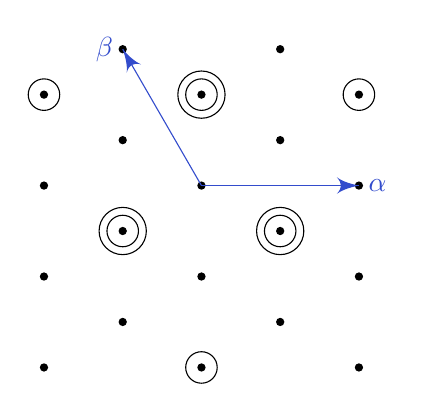
\begin{tikzpicture}
      \foreach \x in {-2, 0, 2} {
        \foreach \y in {0, 1.155, -1.155, -2.310} {
          \node [circ] at (\x, \y) {};
        }
      }
      \foreach \x in {-1, 1} {
        \foreach \y in {0.577, -0.577, 1.732, -1.732} {
          \node [circ] at (\x, \y) {};
        }
      }
      \draw [mblue, ->] (0, 0) -- (2, 0) node [right] {$\alpha$};
      \draw [mblue, ->] (0, 0) -- (-1, 1.732) node [left] {$\beta$};

      \draw (0, 1.155) circle [radius=0.2];
      \draw (0, 1.155) circle [radius=0.3];
      \draw (2, 1.155) circle [radius=0.2];
      \draw (-2, 1.155) circle [radius=0.2];
      \draw (1, -0.577) circle [radius=0.2];
      \draw (-1, -0.577) circle [radius=0.2];
      \draw (1, -0.577) circle [radius=0.3];
      \draw (-1, -0.577) circle [radius=0.3];
      \draw (0, -2.310) circle [radius=0.2];
    \end{tikzpicture}
  \end{center}
  So we see that we have a highest weight of $(2, 0)$. We then use the algorithm to compute all the weights of such an irrep, remove it from the weight lattice, and be left with
  \begin{center}
    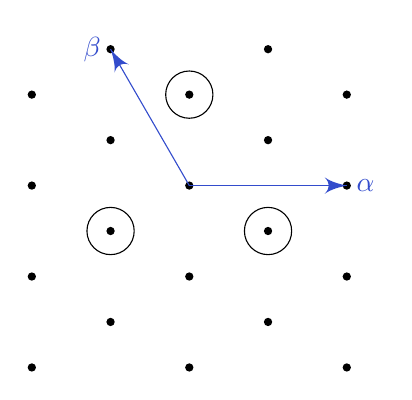
\begin{tikzpicture}
      \foreach \x in {-2, 0, 2} {
        \foreach \y in {0, 1.155, -1.155, -2.310} {
          \node [circ] at (\x, \y) {};
        }
      }
      \foreach \x in {-1, 1} {
        \foreach \y in {0.577, -0.577, 1.732, -1.732} {
          \node [circ] at (\x, \y) {};
        }
      }
      \draw [mblue, ->] (0, 0) -- (2, 0) node [right] {$\alpha$};
      \draw [mblue, ->] (0, 0) -- (-1, 1.732) node [left] {$\beta$};

      \draw (0, 1.155) circle [radius=0.3];
      \draw (1, -0.577) circle [radius=0.3];
      \draw (-1, -0.577) circle [radius=0.3];
    \end{tikzpicture}
  \end{center}
  This is just the anti-fundamental representation. So we have
  \[
    \mathbf{3} \otimes \mathbf{3} = \mathbf{6} \oplus \bar{\mathbf{3}}.
  \]
\end{eg}

%In our theory of the strong interaction, the quarks carry two $\su(3)$ representations, called $\su(3)_{\mathrm{flavour}}$ and $\su(3)_{\mathrm{color}}$. The quarks have representations $\mathbf{3}, \mathbf{3}$, and the anti-quarks have $\bar{\mathbf{3}}, \bar{\mathbf{3}}$.
%
%Since colour is confined, only singlets appear, i.e.\ things in a $\mathbf{1}$-representation. If we have a quark and an anti-quark, we can form
%\[
% \mathbf{3} \otimes \bar{\mathbf{3}} = \mathbf{1} \oplus \mathbf{8}.
%\]
%So we have a $\mathbf{1}$, and this corresponds to $q \bar{q}$.
%
%If we have three quarks, then we get
%\[
% \mathbf{3} \otimes \mathbf{3} \otimes \mathbf{3} = \mathbf{1} \oplus \cdots.
%\]
%So this is a $qqq$ state.
%

\section{Gauge theories}
We are now going to do something rather amazing. We are going to show that Maxwell's equation is ``forced'' upon us by requiring that our (charged) fields possess something known as a \emph{$\U(1)$} gauge symmetry. We are going to write down essentially the only possible theory under the assumption of this gauge symmetry, and unwrapping it gives us Maxwell's equation.

When we do it for Maxwell's equation, it is not entirely clear that what we wrote down was ``the only possible thing'', but it will be when we try to do it for general gauge theories.

Before we begin, it is important to note that everything we do here has a very nice geometric interpretation in terms of connections on principal $G$-bundles, and there are very good geometric reasons to pick the definitions (and names) we use here. Unfortunately, we do not have the time to introduce all the necessary geometry in order to do so.

\subsection{Electromagnetism and \texorpdfstring{$\U(1)$}{U(1)} gauge symmetry}
In electromagnetism, we had two fields $\mathbf{E}$ and $\mathbf{B}$. There are four Maxwell's equations governing how they behave. Two of them specify the evolution of the field and how they interact with matter, while the other two just tells us we can write the field in terms of a scalar and a vector potential $\Phi, \mathbf{A}$. Explicitly, they are related by
\begin{align*}
  \mathbf{E} &= - \nabla \Phi + \frac{\partial \mathbf{A}}{\partial t}\\
  \mathbf{B} &= \nabla \times \mathbf{A}.
\end{align*}
The choice of potentials is not unique. We know that $\mathbf{E}$ and $\mathbf{B}$ are invariant under the transformations
\begin{align*}
  \Phi &\mapsto \Phi + \frac{\partial \alpha}{\partial t}\\
  \mathbf{A} &\mapsto \mathbf{A} + \nabla \alpha
\end{align*}
for any \emph{gauge function} $\alpha = \alpha(\mathbf{x}, t)$.

Now we believe in relativity, so we should write things as $4$-vectors. It so happens that there are four degrees of freedom in the potentials, so we can produce a $4$-vector
\[
  a_\mu =
  \begin{pmatrix}
    \Phi\\
    A_i
  \end{pmatrix}.
\]
We can then succinctly write the gauge transformations as
\[
  a_\mu \mapsto a_\mu + \partial_\mu \alpha.
\]
We can recover our fields via something known as the \emph{electromagnetic field tensor}, given by
\[
  f_{\mu\nu} = \partial_\mu a_\nu - \partial_\nu a_\mu.
\]
It is now easy to see that $f$ is invariant under gauge transformations. We can expand the definitions out to find that we actually have
\[
  f_{\mu\nu} =
  \begin{pmatrix}
    0 & E_x & E_y & E_z\\
    -E_x & 0 & -B_z & B_y\\
    -E_y & B_z & 0 & -B_x\\
    -E_z & -B_y & B_x & 0
  \end{pmatrix}
\]
So we do recover the electric and magnetic fields this way.

The free field theory of electromagnetism then has a Lagrangian of
\[
  \mathcal{L}_{\mathrm{EM}} = - \frac{1}{4 g^2} f_{\mu\nu} f^{\mu\nu} = \frac{1}{2g^2}(\mathbf{E}^2 - \mathbf{B}^2).
\]
For reasons we will see later on, it is convenient to rescale the $a_\mu$ by
\[
  A_\mu = -i a_\mu \in i\R = \mathcal{L}(\U(1))
\]
and write
\[
  F_{\mu\nu}=-if_{\mu\nu}=\partial_\mu A_\nu-\partial_\nu A_\mu.
\]
Now the magic happens when we want to couple this to matter.

Suppose we have a complex scalar field $\phi: \R^{3, 1} \to \C$ with Lagrangian
\[
  \mathcal{L}_\phi = \partial_\mu \phi^* \partial^\mu \phi - W(\phi^* \phi).
\]
The interesting thing is that this has a \emph{global} $\U(1)$ symmetry by
\begin{align*}
  \phi &\mapsto g \phi\\
  \phi^* &\mapsto g^{-1}\phi^*
\end{align*}
for $g = e^{i\delta} \in \U(1)$, i.e.\ the Lagrangian is invariant under this action.

In general, it is more convenient to talk about infinitesimal transformations Consider an element
\[
  g = \exp(X) \approx 1 + X,
\]
where we think of $X$ as ``small''. In our case, we have $X \in \uu(1) \cong i\R$, and
\begin{align*}
  \phi &\mapsto \phi + \delta_X \phi,\\
  \phi^* &\mapsto \phi ^*+ \delta_X \phi^*,
\end{align*}
where
\begin{align*}
  \delta_X \phi &= X \phi\\
  \delta_X \phi^* &= -X \phi^*.
\end{align*}
Now this is a \emph{global} symmetry, i.e.\ this is a symmetry if we do the same transformation at all points in the space. Since we have
\[
  \delta_X \mathcal{L}_\phi = 0,
\]
we get a conserved charge. What if we want a \emph{local} symmetry? We want to have a different transformation at \emph{every} point in space, i.e.\ we now have a function
\[
  g: \R^{3, 1} \to \U(1),
\]
and we consider the transformations given by
\begin{align*}
  \phi(x) &\mapsto g(x) \phi(x)\\
  \phi^*(x) &\mapsto g^{-1}(x) \phi^*(x).
\end{align*}
This is in general no longer a symmetry. Under an infinitesimal variation $X: \R^{3, 1} \to \uu(1)$, we have
\[
  \delta_X \phi = X \phi.
\]
So the derivative transforms as
\[
  \delta_X (\partial_\mu \phi) = \partial_\mu (\delta_X \phi) = (\partial_\mu X) \phi + X \partial_\mu \phi.
\]
This is bad. What we really want is for this to transform like $\phi$, so that
\[
  \partial_\mu \phi \mapsto g(x) \partial_\mu \phi.
\]
Then the term $\partial_\mu \phi^* \partial^\mu \phi$ will be preserved.

It turns out the solution is to couple $\phi$ with $A_\mu$. Recall that both of these things had gauge transformations. We now demand that under any gauge transformation, both should transform the same way. So from now on, a gauge transformation $X: \R^{3, 1} \to \uu(1)$ transforms \emph{both} $\phi$ and $A_\mu$ by
\begin{align*}
  \phi &\mapsto \phi + X \phi\\
  A_\mu &\mapsto A_\mu - \partial_\mu X.
\end{align*}
However, this does not fix the problem, since everything we know so far that involves the potential $A$ is invariant under gauge transformation. We now do the funny thing. We introduce something known as the \emph{covariant derivative}:
\[
  \D_\mu = \partial_\mu + A_\mu,
\]
Similar to the case of general relativity (if you are doing that course), the covariant derivative is the ``right'' notion of derivative we should use whenever we want to differentiate fields that are coupled with $A$. We shall now check that this derivative transforms in the same way as $\phi$. Indeed, we have
\begin{align*}
  \delta_X(\D_\mu \phi) &= \delta_X(\partial_\mu \phi + A_\mu \phi)\\
  &= \partial_\mu (\delta_X \phi) + A_\mu \delta_X \phi - \partial_\mu X \phi\\
  &= X \partial_\mu \phi + X A_\mu \phi\\
  &= X \D_\mu \phi.
\end{align*}
This implies that the kinetic term
\[
  (\D_\mu \phi)^* \D^\mu \phi
\]
is gauge invariant. So we can put together a gauge-invariant Lagrangian
\[
  \mathcal{L} = -\frac{1}{4 g^2} F_{\mu\nu} F^{\mu\nu} + (\D_\mu \phi)^* (\D^\mu \phi) - W(\phi^* \phi).
\]
So what the electromagnetic potential $A$ gives us is a covariant derivative $\D$ which then allows us to ``gauge'' these complex fields to give them a larger symmetry group.

\subsection{General case}
We now want to do what we had above for a general Lie group $G$. In particular, this can be non-abelian, and thus the Lie algebra has non-trivial bracket. It turns out in the general case, it is appropriate to insert some brackets into what we have done so far, but otherwise most things follow straight through.

In the case of electromagnetism, we had a Lie group $\U(1)$, and it acted on $\C$ in the obvious way. In general, we start with a Lie group $G$, and we have to pick a representation $D$ of $G$ on a vector space $V$. Since we want to have a real Lagrangian, we will assume our vector space $V$ also comes with an inner product.

Given such a representation, we consider fields that take values in $V$, i.e.\ functions $\phi: \R^{3, 1} \to V$. We can, as before, try to write down a (scalar) Lagrangian
\[
  \mathcal{L}_\phi = (\partial_\mu \phi, \partial^\mu \phi) - W((\phi, \phi)).
\]
Writing out the summation explicitly, we have
\[
  \mathcal{L}_\phi = \sum_{\mu = 0}^3 (\partial_\mu \phi, \partial^\mu \phi) - W((\phi, \phi)),
\]
i.e.\ the sum is performed outside the inner product.

This is not always going to be invariant under an arbitrary action of the group $G$, because the inner product is not necessarily preserved. Fortunately, by definition of being unitary, what we require is that our representation is \emph{unitary}, i.e.\ each $D(g)$ is unitary for all $g \in G$.

It is a theorem that any representation of a compact Lie group is equivalent to one that is unitary, so we are not losing too much by assuming this (it is also that a non-compact Lie group cannot have a non-trivial unitary representation).

Again, it will be convenient to think about this in terms of infinitesimal transformations. Near the identity, we can write
\[
  g = \exp(X)
\]
for some $X \in \mathfrak{g}$. Then we can write
\[
  D(g) = \exp(\rho(X)) \in \gl(n, \C).
\]
We write $\rho: \mathfrak{g} \to \gl(n, \C)$ for the associated representation of the Lie algebra $\mathfrak{g}$. If $D$ is unitary, then $\rho$ will be anti-Hermitian. Then the infinitesimal transformation is given by
\[
  \phi \mapsto \phi + \delta_X \phi = \phi + \rho(X) \phi.
\]
In general, an infinitesimal Gauge transformation is then given by specifying a function
\[
  X: \R^{3, 1} \to \mathfrak{g}.
\]
Our transformation is now
\[
  \delta_X \phi = \rho(X(x))\phi.
\]
Just as in the abelian case, we know our Lagrangian is no longer gauge invariant in general.

We now try to copy our previous fix. Again, we suppose our universe comes with a gauge field
\[
  A_\mu : \R^{3, 1} \to \mathcal{L}(G).
\]
Again, we can define a covariant derivative
\[
  \D_\mu \phi = \partial_\mu \phi + \rho(A_\mu) \phi.
\]
In the case of a non-abelian gauge symmetry, our gauge field transformed under $X$ as
\[
  \delta_X A_\mu = - \partial_\mu X.
\]
This expression still makes sense, but it turns out this isn't what we want, if we try to compute $\delta_X(\D_\mu \phi)$. Since the gauge field is non-abelian, there is one extra thing we can include, namely $[X, A_\mu]$. It turns out this is the right thing we need. We claim that the right definition is
\[
  \delta_X A_\mu = - \partial_\mu X + [X, A_\mu].
\]
To see this, we show that
\begin{prop}
  We have
  \[
    \delta_X (\D_\mu \phi) = \rho(X) \D_\mu \phi.
  \]
\end{prop}

The proof involves writing out the terms and see that it works.
\begin{proof}
  We have
  \begin{align*}
    \delta_X (\D_\mu \phi) &= \delta_X(\partial_\mu \phi + \rho(A_\mu) \phi)\\
    &= \partial_\mu (\delta_X\phi) + \rho(A_\mu) \delta_X \phi + \rho(\delta_X A_\mu)\phi\\
    &= \partial_\mu (\rho(X) \phi) + \rho(A_\mu) \rho(X) \phi - \rho(\partial_\mu X) \phi + \rho([X, A_\mu]) \phi\\
    &= \rho(\partial_\mu X) \phi + \rho(X) \partial_\mu \phi + \rho(X)\rho(A_\mu) \phi \\
    &\quad\quad+ [\rho(A_\mu), \rho(X)] \phi - \rho(\partial_\mu X) \phi + \rho([X, A_\mu])\phi\\
    &= \rho(X)(\partial_\mu \phi + \rho(A_\mu) \phi)\\
    &= \rho(X) \D_\mu \phi,
  \end{align*}
  as required.
\end{proof}

Thus, we know that $(\D_\mu \phi, \D^\mu \phi)$ is gauge invariant. We can then write down a gauge invariant ``matter'' part of the action
\[
  \mathcal{L}_\phi = (\D_\mu \phi, \D^\mu \phi) - W[(\phi, \phi)].
\]
Finally, we need to produce a gauge invariant kinetic term for $A_\mu: \R^{3, 1} \to \mathcal{L}(G)$.

For the case of an abelian gauge theory, we had
\[
  F_{\mu\nu} = \partial_\mu A_\nu - \partial_\nu A_\mu \in \mathcal{L}(G).
\]
In this case, there is one extra term we can add, namely $[A_\mu, A_\nu] \in \mathfrak{g}$, and it turns out we need it for things to work out. Our field strength tensor is
\[
  F_{\mu\nu} = \partial_\mu A_\nu - \partial_\nu A_\mu + [A_\mu, A_\nu].
\]
How does the field strength tensor transform? In the abelian case, we had that $F_{\mu\nu}$ was invariant. Let's see if that is the case here. It turns out this time the field strength tensor transforms as the adjoint representation.
\begin{lemma}
  We have
  \[
    \delta_X (F_{\mu\nu}) = [X, F_{\mu\nu}] \in \mathcal{L}(G).
  \]
\end{lemma}

\begin{proof}
  We have
  \begin{align*}
    \delta_X(F_{\mu\nu}) &= \partial_\mu (\delta_X A_\nu) - \partial_\nu (\delta_X A_\mu) + [\delta_X A_\mu, A_\nu] + [A_\mu, \delta_X A_\nu]\\
    &= \partial_\mu \partial_\nu X + \partial_\mu ([X, A_\nu]) - \partial_\nu \partial_\mu X - \partial_\nu ([X, A_\mu]) - [\partial_\mu X, A_\nu]\\
    &\quad\quad- [A_\mu, \partial_\nu X] + [[X, A_\mu ], A_\nu] + [A_\mu, [X, A_\nu]]\\
    &= [X, \partial_\mu A_\nu] - [X, \partial_\nu A_\mu] +([X, [A_\mu, A_n]]\\
    &= [X, F_{\mu\nu}].
  \end{align*}
  where we used the Jacobi identity in the last part.
\end{proof}

So to construct a scalar quantity out of $F_{\mu\nu}$, we need an inner product invariant under an adjoint representation. We know one of these --- the Killing form! So we can just pick
\[
  \mathcal{L}_A = \frac{1}{g^2} \kappa(F_{\mu\nu}, F^{\mu\nu}).
\]
This is known as the \emph{Yang-Mills Lagrangian}. Note that for each fixed $\mu, \nu$, we have that $F_{\mu\nu} \in \mathfrak{g}$. So we should read this as
\[
  \mathcal{L}_A = \frac{1}{g^2} \sum_{\mu, \nu} \kappa(F_{\mu\nu}, F^{\mu\nu}).
\]
Putting all these together, we get ourselves an invariant Lagrangian of the system with a $G$ gauge symmetry.

So the final Lagrangian looks like
\[
  \mathcal{L} = \frac{1}{g^2} \sum_{\mu, \nu} \kappa(F_{\mu\nu}, F^{\mu\nu}) + (\D_\mu \phi, \D^\mu \phi) + W((\phi, \phi)).
\]
Now if we are further told that we actually have a simple complex Lie algebra, then it is a fact that we can find a real form of compact type. So in particular we can find a basis $\mathcal{B} = \{T^a, a = 1, \cdots, \dim \mathfrak{g}\}$ with
\[
  \kappa^{ab} = \kappa(T^a, T^b) = - \kappa \delta^{ab}.
\]
In this basis, we have
\[
  \mathcal{L}_A = \frac{-\kappa}{g^2} \sum_{a = 1}^d F_{\mu\nu, a} F^{\mu\nu, a},
\]
and this does look like a copy of $d$ many electromagnetic fields.

So to construct (a sensible) gauge theory, we need to get a (semi-)simple Lie algebra, and then find some representations of $\mathfrak{g}$. These are things we have already studied well before!

According to our current understanding, the gauge group of the universe is
\[
  G = \U(1) \times \SU(2) \times \SU(3),
\]
and, for example, the Higgs boson has representation
\[
  \phi = (+1, \rho_1, \rho_0).
\]

\section{Lie groups in nature}
We are now going to look around and see how the things we have done exhibit themselves in nature. This chapter, by design, is very vague, and one shall not expect to learn anything concrete from here.

\subsection{Spacetime symmetry}
In special relativity, we have a metric
\[
  \d s^2 = -\d t^2 + \d x^2 + \d y^2 + \d z^2.
\]
The group of (orientation-preserving and) metric-preserving symmetries gives us the \term{Lorentz group} $\SO(3, 1)$. However, in certain cases, we can get something more (or perhaps less) interesting. Sometimes it makes sense to substitute $\tau = i t$, so that
\[
  \d s^2 = \d \tau^2 + \d x^2 + \d y^2 + \d z^2.
\]
This technique is known as \term{Wick rotation}. If we put it this way, we now have a symmetry group of $\SO(4)$ instead.

It happens that when we complexify this, this doesn't really matter. The resulting Lie algebra is
\[
  \mathcal{L}_\C(\SO(3, 1)) = \mathcal{L}_\C(\SO(4)) = D_2.
\]
Its Dynkin diagram is
\begin{center}
  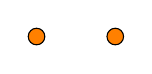
\begin{tikzpicture}
      \foreach \x in {0,1} {
        \node [draw, fill=morange, circle, inner sep = 0, minimum size = 6] at (\x, 0) {};
      }
  \end{tikzpicture}
\end{center}
This is not simple, and we have
\[
  D_2 = A_1 \oplus A_1.
\]
In other words, we have
\[
  \so(4) = \su(2) \oplus \su(2).
\]
At the Lie group level, $\SO(4)$ does not decompose as $\SU(2) \times \SU(2)$. Instead, $\SU(2) \times \SU(2)$ is a double cover of $\SO(4)$, and we have
\[
  \SO(4) = \frac{\SU(2) \times \SU(2)}{\Z_2}.
\]
Now in general, our fields in physics transform when we change coordinates. There is the boring case of a scalar, which never transforms, and the less boring case of a vector, which transforms like a vector. More excitingly, we have objects known as spinors. The weird thing is that spinors do have an $\so(3, 1)$ action, but this does not lift to an action of $\SO(3, 1)$. Instead, we need to do something funny with double covers, which we shall not go into.

In general, spinors decompose into ``left-handed'' and ``right-handed'' components, known as \emph{Weyl fermions}, and these correspond to two different representations of $A_1$. We can summarize the things we have in the following table:
\begin{center}
  \begin{tabular}{ccc}
    \toprule
    Field & $\so(3, 1)$ & $A_1 \oplus A_1$\\
    \midrule
    Scalar & $\mathbf{1}$ & $(\rho_0, \rho_0)$\\
    Dirac Fermion & LH $\oplus$ RH & $(\rho_1, \rho_0) \oplus (\rho_0, \rho_1)$\\
    Vector & $\mathbf{4}$ & $(\rho_1, \rho_1)$\\
    \bottomrule
  \end{tabular}
\end{center}
However, the Lorentz group $\SO(3, 1)$ is not all the symmetries we can do to Minkowski spacetime. These are just those symmetries that fix the origin. If we add in the translations, then we obtain what is known as the \term{Poincar\'e group}. The Poincar\'e algebra is \emph{not} simple, as the translations form a non-trivial ideal.

\subsection{Possible extensions}
Now we might wonder how we can expand the symmetry group of our theory to get something richer. In very special cases, we will get what is known as \emph{conformal symmetry}, but in general, we don't. To expand the symmetry further, we must consider supersymmetry.
\subsubsection*{Conformal field theory}
If all our fields are massless, then our theory gains \term{conformal invariance}. Before we look into conformal invariance, we first have a look at a weaker notion of scale invariance.

A massless free field $\phi: \R^{3, 1} \to V$ has a Lagrangian that looks like
\[
  \mathcal{L} = -\frac{1}{2}(\partial_\mu \phi, \partial^\mu \phi).
\]
This is invariant under scaling, namely the following simultaneous transformations parameterized by $\lambda$:
\begin{align*}
  x &\mapsto x' = \lambda^{-1} x\\
  \phi(x) &\mapsto \lambda^\Delta \phi(x'),
\end{align*}
where $\Delta = \dim V$ is the dimension of the field.

Often in field theory, whenever we have scale invariance, we also get \emph{conformal} invariance. In general, a conformal transformation is one that preserves all angles. So this, for example, includes some mixture and scaling, and is more general than Lorentz invariance and scale invariance.

In the case of 4 (spacetime) dimensions, it turns out the conformal group is $\SO(4, 2)$, and has dimension $15$. In general, members of this group can be written as
\[
  \begin{pmatrix}
    \begin{matrix}
      0 & D\\
      -D & 0\\
    \end{matrix} & P_\mu + K_\mu\\
    P_\nu + K_\nu & \begin{matrix} & & \\ & \mathcal{M}_{\mu\nu} & \\ & & &\end{matrix}
  \end{pmatrix}.
\]
Here the $K_\mu$ are the \term{special conformal generators}, and the $P_\mu$ are translations. We will not go deep into this.

Conformal symmetry gives rise to \term{conformal field theory}. Theoretically, this is very important, since they provide ``end points'' of renormalization group flow. This will be studied more in depth in the Advanced Quantum Field Theory course.

\subsubsection*{Supersymmetry}
Can we add even more symmetries? It turns out there is a no-go theorem that says we can't.
\begin{thm}[Coleman-Mondula]
  In an interactive quantum field theory (satisfying a few sensible conditions), the largest possible symmetry group is the Poincar\'e group times some internal symmetry that commutes with the Poincar\'e group.
\end{thm}
But this is not the end of the world. The theorem assumes that we are working with traditional Lie groups and Lie algebras. The idea of supersymmetry is to prefix everything we talk about with ``super-'', so that this theorem no longer applies.

To being with, supersymmetry replaces Lie algebras with graded Lie algebras, or \term{Lie superalgebras}. This is a graded vector space, which we can write as
\[
  \mathfrak{g} = \mathfrak{g}_0 \oplus \mathfrak{g}_1,
\]
where the elements in $\mathfrak{g}_0$ as said to have \emph{grade} $0$, and elements in $\mathfrak{g}_1$ have grade $1$. We write $|X| = 0, 1$ for $X \in \mathfrak{g}_0, \mathfrak{g}_1$ respectively. These will correspond to bosonic and fermionic operators respectively.

Now the Lie bracket respects a graded anti-commutation relation
\[
  [X, Y] = -(-1)^{|X||Y|}[Y, X].
\]
So for Bosonic generators, they anti-commute as usual, but with we have two fermionic things, they commute. We can similarly formulate a super-Jacobi identity. These can be used to develop field theories that have these ``supersymmetries''.

Unfortunately, there is not much experimental evidence for supersymmetry, and unlike string theory, we are already reaching the scales we expect to see supersymmetry in the LHC\ldots

\subsection{Internal symmetries and the eightfold way}
Finally, we get to the notion of internal symmetries. Recall that for a complex scalar field, our field was invariant under a global $\U(1)$ action given by phase change. More generally, fields can carry some representation of a Lie group $G$. In general, if this representation has dimension greater than $1$, this means that we have multiple different ``particles'' which are related under this symmetry transformation. Then by symmetry, all these particles will have the same mass, and we get a degeneracy in the mass spectrum.

When we have such degeneracies, we would want to distinguish the different particles of the same mass. These can be done by looking at the weights of the representation. It turns out the different weights correspond to the different quantum numbers of the particles.

Often, we do not have an exact internal symmetry. Instead, we have an approximate symmetry. This is the case when the dominant terms in the Lagrangian are invariant under the symmetry, while some of the lesser terms are not. In particular, the different particles usually have different (but very similar) masses.

These internal symmetries are famously present in the study of hadrons, i.e.\ things made out of quarks. The basic examples we all know are the nucleons, namely protons and neutrons. We can list them as
\begin{center}
  \begin{tabular}{ccc}
    \toprule
    & Charge (Q) & Mass (M)\\
    \midrule
    $p$ & $+1$ & $938$ MeV\\
    $n$ & $0$ & $940$ MeV\\
    \bottomrule
  \end{tabular}
\end{center}
Note that they have very similar masses. Later, we found, amongst many other things, the pions:
\begin{center}
  \begin{tabular}{ccc}
    \toprule
    & Charge (Q) & Mass (M)\\
    \midrule
    $\pi^+$ & +1 & 139 MeV\\
    $\pi^0$ & 0 & 135 MeV\\
    $\pi^-$ & -1 & 139 MeV\\
    \bottomrule
  \end{tabular}
\end{center}
Again, these have very similar masses. We might expect that there is some approximate internal symmetry going on. This would imply that there is some conserved quantity corresponding to the weights of the representation. Indeed, we later found one, known as \emph{isospin}:
\begin{center}
  \begin{tabular}{cccc}
    \toprule
    & Charge (Q) & Isospin (J) & Mass (M)\\
    \midrule
    $p$ & $+1$ & $+\frac{1}{2}$ & $938$ MeV\\
    $n$ & $0$ & $-\frac{1}{2}$ & $940$ MeV\\
    $\pi^+$ & +1 & +1 & 139 MeV\\
    $\pi^0$ & 0 & 0 & 135 MeV\\
    $\pi^-$ & -1 & -1 & 139 MeV\\
    \bottomrule % check numbers
  \end{tabular}
\end{center}
Isospin comes from an approximate $\SU(2)_I$ symmetry, with a generator given by
\[
  H = 2J.
\]
The nucleons then have the fundamental $\rho_1$ representation, and the pions have the $\rho_2$ representation.

Eventually, we got smarter, and discovered an extra conserved quantum number known as \emph{hypercharge}. We can plot out the values of the isospin and the hypercharge for our pions and some other particles we discovered, and we found a pattern:
\begin{center}
  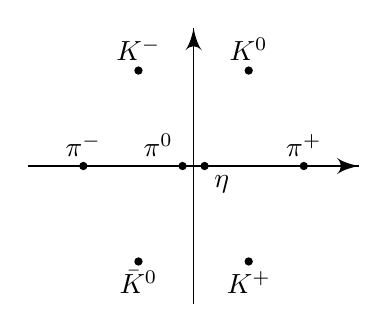
\begin{tikzpicture}[scale=0.7]
    \draw [->] (-3, 0) -- (3, 0);
    \draw [->] (0, -2.5) -- (0, 2.5);
    \node [circ] at (2, 0) {};
    \node [above] at (2, 0) {$\pi^+$};
    \node [circ] at (1, 1.732) {};
    \node [above] at (1, 1.732) {$K^0$};
    \node [circ] at (1, -1.732) {};
    \node [below] at (1, -1.732) {$K^+$};
    \node [circ] at (-2, 0) {};
    \node [above] at (-2, 0) {$\pi^-$};
    \node [circ] at (-1, 1.732) {};
    \node [above] at (-1, 1.732) {$K^-$};
    \node [circ] at (-1, -1.732) {};
    \node [below] at (-1, -1.732) {$\bar K^0$};
    \node [circ] at (-0.2, 0) {};
    \node [anchor = north west] at (0.2, 0) {$\eta$};
    \node [circ] at (0.2, 0) {};
    \node [anchor = south east] at (-0.2, 0) {$\pi^0$};
  \end{tikzpicture}
\end{center}
At firsts, physicists were confused by the appearance of this pattern, and tried very hard to figure out generalizations. Of course, now that we know about Lie algebras, we know this is the weight diagram of a representation of $\su(3)$.

However, the word $\SU(3)$ hasn't resolved all the mystery. In reality, we only observed representations of dimension $1, 8$ and $10$. We did not see anything else. So physicists hypothesized that there are substructures known as quarks. Each quark ($q$) carry a $\mathbf{3}$ representation (flavour), and antiquarks ($\bar{q}$) carry a $\bar{\mathbf{3}}$ representation.

The mesons correspond to $q\bar{q}$ particles, and the representation decompose as
\[
  \mathbf{3} \otimes \bar{\mathbf{3}} = \mathbf{1} \oplus \mathbf{8}.
\]
Bosons correspond to $qqq$ particles, and these decompose as
\[
  \mathbf{3} \otimes \mathbf{3} \otimes \mathbf{3} = \mathbf{1} \oplus \mathbf{8} \oplus \mathbf{8} \oplus \mathbf{10}.
\]
Of course, we now have to explain why only $q\bar{q}$ and $qqq$ appear in nature, and why we don't see quarks appearing isolated in nature. To do so, we have to go very deep down in QCD. This theory says that quarks have a $\SU(3)$ gauge symmetry (which is a different $\SU(3)$) and the quark again carries the fundamental representation $\mathbf{3}$. More details can be found in the Lent Standard Model course.
\printindex
\end{document}
